\documentclass[12pt, oneside] {report} % Use the report class with 12pt font 
\usepackage[utf8]{inputenc} % Character encoding
\usepackage[T1]{fontenc} % Support for characters like « and »
\usepackage{lmodern} % Fixes font generation errors
\usepackage{hyperref} % For hyperlinks
\usepackage{geometry} % For margin settings
\usepackage{textcomp}  % Include this package to use \textcopyright
\usepackage{graphicx} % For handling images
\usepackage{cite} % For citations
\usepackage{xcolor} 
\usepackage{amsmath,amssymb,amsfonts} % For math fonts, symbols and environments
\usepackage{algorithmic} % For algorithms
\usepackage{fancyhdr} % For fancy headers
\usepackage{nomencl} % For the nomenclature
\usepackage{appendix} % For appendices
\usepackage{tocloft} % For table of contents customization
\usepackage{tabularx}
\usepackage[table]{xcolor} % for colors
\usepackage{longtable}
\usepackage{tabularx} % for X column type
\usepackage{tabularray}
\usepackage{subcaption}
% \UseTblrLibrary{booktabs,longtable}
\usepackage{booktabs}
\usepackage{longtable}
\usepackage{geometry}
\usepackage{svg}
\geometry{margin=1in}
\hypersetup{ % Setup hyperlinks
    colorlinks=true,
    citecolor=black,
    linkcolor=black,
    urlcolor=black,
    pdftitle={PhD Thesis},
    pdfauthor={Author Name}
}

\makenomenclature
\renewcommand{\nomname}{List of Abbreviations}

\pagestyle{fancy}
\fancyhf{}
\fancyhead[LE,RO]{\thepage}
\fancyhead[RE]{\nouppercase{\leftmark}}
\fancyhead[LO]{\nouppercase{\rightmark}}

\renewcommand{\bibname}{References}  % For book, report, and thesis classes

\usepackage{titlesec}
\usepackage{booktabs}
\usepackage{rotating}  % Enables sidewaystable environment

% For subfigures
\usepackage{caption}
\usepackage{subcaption}

\begin{document}

\pagenumbering{roman} % Use roman numerals for front matter
% Title Page
%Title page one
\begin{titlepage}
    \centering
    
\includegraphics[width=1\textwidth]{images/Logo2.png}\\[0.4cm] % University Logo
% \includegraphics[width=1\textwidth]{images/Logo.png}\\[0.1in]
% \vspace{2em}%

\includegraphics[height=0.2cm, width=\textwidth]{images/red _line.png}\\[0.2cm]
    % {\huge \textsc{Makerere University}}\\[1cm] % University Name
     
    % Title with custom formatting
    % \textcolor[HTML]{000080}{\MakeUppercase{\Large College of Computing and Information Science}}\\[20]

    \\[0.5cm] 
    {\textbf{ \Large Traxis: Taxi Coordination Application System for Uganda’s Public Transport Sector}
    \\[0.5cm]
    
    {by}\\[0.5cm]
    {\textbf{\large Group 7}\\[0.5cm]
    \textbf{Department of Computer Science}\\[0.1cm]
    \textbf{School of Computing & Informatics Technology
    }\\
    \\[1cm]% Author Name
   \textit{A Project Proposal Submitted to the School of Computing and Informatics Technology for the Study Leading to a Project Report in Partial Fulfilment of the requirements for the Award of the Degree of Bachelor of Science in Computer Science of Makerere University}

\\[1.5cm]
    
    \textbf{\large Supervisor}\\
    \text{Dr. Marriette Katarahweire} \\[1.0cm]
    % \textbf{Co-supervisor's Name}\\[1cm]
    
 {\large
\textbf{Department of Computer Science} \\[0.1cm]
\textbf{School of Computing \& Informatics Technology} \\[0.1cm] 
\textbf{kmarriette@cit.ac.ug Tel: +256414540628}
}\\[0.5cm]
\text{November 2025}
    
\end{titlepage}    % November 2025 % Date







\chapter*{Declaration}
\addcontentsline{toc}{chapter}{Declaration} % Adds this chapter to the table of contents
We, Group 7 do hereby declare that this Project Proposal is original and has not been published and/or submitted for any other degree award to any other University before.

\vspace{1.5cm}

% Table with controlled column widths
{\fontfamily{ptm}\selectfont
\begin{tabular}{|p{1cm}|p{6cm}|p{4.5cm}|p{3cm}|}
\hline
\textbf{SNo} & \textbf{Names} & \textbf{Registration Number} & \textbf{Signature} \\
\hline
1 & Sunday Emmanuel Hezekiah & 23/X/23054/PS & \\[0.3cm]
\hline
2 & Mulindwa Mark Myles & 23/U/11949/PS & \\[0.3cm]
\hline
3 & Naluwujja Ashley Hope & 23/U/14174/PS & \\[0.3cm]
\hline
4 & Kiggundu Sulaiman & 22/U/21927/PS & \\[0.3cm]
\hline
\end{tabular}
}

\vspace{2cm}

\noindent
\textbf{Date:}\\
\rule{8cm}{0.4pt}

\vspace{3cm}
\chapter*{Approval}
\addcontentsline{toc}{chapter}{Approval} 
% \noindent
% \textbf{\Large Approval}

\vspace{0.3cm}

This Project Proposal has been submitted for examination with the approval of the following supervisor.

\vspace{0.5cm}
\noindent
\textbf{Signed:}\\
\rule{8cm}{0.4pt}

\vspace{0.3cm}
\noindent
\textbf{Date:}\\
\rule{8cm}{0.4pt}

\vspace{0.5cm}
\noindent
\textbf{Dr. Marriette Katarahweire} \\
School of Computing \& IT \\
College of Computing \& IT \\
Makerere University \\
kmarriette@cit.ac.ug

% Move signature section to bottom left
% \vfill
% \noindent
% \textbf{Signed:} \underline{\hspace{5cm}}

% \vspace{0.5cm}
% \noindent
% \textbf{Date:} \underline{\hspace{3cm}}

% \begin{flushleft}
% \vspace{1cm}
% \textbf{Supervisors:}

% Supervisor's Name \hfill \textit{Sign:}\underline{\hspace{4cm}}\textit{Date:}\underline{\hspace{4cm}} 

% \vspace{1.0cm}
% Co-supervisor's Name \hfill \textit{Sign:}\underline{\hspace{4cm}} \textit{Date:}\underline{\hspace{4cm}}   
% \end{flushleft}







\chapter*{Dedication}
\addcontentsline{toc}{chapter}{Dedication} 
We dedicate this report to the Almighty God without whom, we could have done nothing. We further dedicate this report to our parents and guardians for the unceasing and selfless support throughout our stay in the University.
\chapter*{Acknowledgements}
\addcontentsline{toc}{chapter}{Acknowledgements} % Adds this chapter to the table of contents
We would like to express our sincere gratitude to our project supervisor, Dr. Marriette Katarahweire, for her invaluable guidance and feedback during the preparation of this proposal. Her insights have been instrumental in shaping the direction of our research, and we look forward to her continued mentorship throughout the project's development.

We also extend our thanks in advance to the taxi drivers, conductors, and commuters in Kampala who will participate in our interviews and surveys. Their willingness to share their experiences and challenges will be fundamental to defining the requirements for the Traxis application.

% Our appreciation goes to our families and friends for their anticipated support and understanding during the demanding phases of this project.

Furthermore, we acknowledge the Department of Computer Science at Makerere University for providing the academic framework and resources that will enable this research.

Finally, we recognize the crucial role that open-source technologies and frameworks will play in the development of the Traxis system.

\chapter*{Abstract}
\addcontentsline{toc}{chapter}{Abstract} 

Private shuttle transportation services in Uganda, particularly on intercity routes such as Kampala–Kabale, face significant challenges related to coordination, booking management, and operational efficiency. These services largely rely on manual processes, including phone-based bookings and informal passenger coordination, which result in inefficiencies such as unreliable seat allocation, unutilized capacity, and limited visibility for both operators and passengers.

This study addressed these challenges through the design and development of Traxis, a mobile application aimed at improving the organization and efficiency of private shuttle operations. The system was designed to support seat-based booking, real-time vehicle and occupancy tracking, and structured scheduling of shuttle services. It also incorporated features for managing passenger information, monitoring vehicle movement, and facilitating communication between operators and users.

Traxis adopted a dual-interface approach, providing functionality for both passengers and operators. Passengers were able to search for available routes, book specific seats, and receive real-time updates, while operators were able to monitor trips, track vehicle activity, and manage bookings through an administrative dashboard. The system design emphasized usability and accessibility to accommodate users with varying levels of digital literacy.

The project demonstrated the potential of mobile technology to improve coordination and resource utilization within privately operated shuttle services. By introducing structured booking, real-time tracking, and integrated operational management, Traxis provided a scalable and context-aware solution for enhancing efficiency, transparency, and reliability in Uganda’s intercity transport sector.


\newpage
% Table of Contents
\tableofcontents
\listoffigures
\listoftables
\newpage

% Main Content
\pagenumbering{arabic} % Use arabic numerals for main content

% Include chapters
\chapter{Introduction}
\label{chap:introduction}

\section{Background to the Study}
Public transportation remains a critical component of mobility in Uganda, particularly in rapidly growing urban centers such as Kampala \cite{mak2026kampala}. While traditional taxi systems (matatus) serve a large portion of the population, there has been a growing demand for more reliable, comfortable, and organized transport alternatives \cite{rugamba2020lowcarbon}. Private shuttle services have emerged to fill this gap by offering scheduled trips, reduced overcrowding, and improved travel experiences. Despite these advantages, many of these services still operate with limited technological support \cite{bmau2025transport}.

Private shuttle operators often rely on manual processes such as phone calls and informal record-keeping to manage bookings, communicate with passengers, and coordinate trips. This approach presents several challenges, including double bookings, customer no-shows, difficulty in tracking seat availability, and inefficiencies in managing routes and schedules \cite{masinde2024uganda}. Additionally, customers may face challenges in accessing these services, as they are often only known through referrals or local advertisements, limiting their reach and accessibility.

The lack of a centralized digital platform also affects courier services offered by these operators. Package delivery coordination, pricing, and tracking are typically handled manually, making it difficult to provide real-time updates and efficient service \cite{itd2026couriercomparison}. This results in frequent customer inquiries, operational delays, and missed opportunities for optimizing vehicle usage.

With the increasing penetration of smartphones and mobile internet in Uganda \cite{ucc2024sectorreport}, there is a significant opportunity to enhance the operations of private transport services through technology. Mobile applications that support features such as seat booking, digital payments, real-time tracking, and automated communication can greatly improve both customer experience and operational efficiency \cite{vocal2026busbooking}, \cite{sayyed2024mobilecx}.

This project proposes the development of a mobile application, Traxis, aimed at supporting private shuttle and courier service providers. The system will enable users to easily discover available services, book seats, select preferred seating positions, and track journeys or deliveries in real time. For operators, the application will provide tools for managing bookings, monitoring vehicle movement, tracking revenue, and optimizing capacity utilization. By introducing a structured and user-friendly digital platform, the system aims to improve reliability, accessibility, and overall service delivery within the private transport sector in Uganda.

\section{Problem Statement}
Private shuttle transport services in Uganda, particularly in urban centers like Kampala, face significant challenges related to coordination and service management despite offering a more reliable alternative to traditional public transport. These challenges result in inefficiencies such as limited service visibility, difficulties in accessing booking information, customer no-shows, and underutilization of available seating capacity. The reliance on manual processes, such as phone calls and informal scheduling, further complicates operations and limits the ability of service providers to effectively manage passenger demand.

The absence of a structured, technology-enabled platform to support real-time booking, seat allocation, and service coordination exacerbates these issues. Consequently, customers often experience inconvenience and uncertainty when trying to access these services, while operators face operational inefficiencies that can lead to revenue losses and reduced service quality. Without an accessible and user-friendly digital solution, these challenges will persist, highlighting the need for an application such as Traxis to enhance communication, improve transparency, and optimize the management of private shuttle transport services in Uganda.
\vspace{1cm}
\section{Objectives}
\subsection{Main Objective}
% The main objective of this project is to develop a mobile application that reduces waiting times and increases the average taxi occupancy rates through real-time tracking and scheduled pickups.

The main objective of this project is to design and develop a mobile application (Traxis) that facilitates efficient management of private shuttle and courier transport services. The system will incorporate features such as real-time vehicle tracking, digital seat booking, and passenger scheduling for pickups. This initiative aims to address key operational inefficiencies by improving coordination between service providers and customers, reducing booking-related challenges such as no-shows, and optimizing seat utilization. Ultimately, the application seeks to enhance the reliability, accessibility, and overall efficiency of private transport services.
% 3
% \newpage
\subsection{Specific Objectives}
We aim to achieve the following specific objectives with the project:
\begin{itemize}
    \item[i.]  To gather comprehensive data on passenger requirements, operational challenges faced by private shuttle and courier service providers, and the functionalities of existing transport management systems.
    % To study the existing or related systems in order to ascertain the need for the proposed mobile application.
    
    \item[ii.]To synthesize and analyze the acquired data to define a comprehensive set of system requirements for the Traxis application.
    % To analyse data from taxi personnels as well as the desired customers for a comprehensive set of system requirements for the Traxis application.
    
    
    \item[iii.] To design and implement the proposed mobile application with all core feautures.
    
    \item[iv.] 
    % To test and validate the system's performance and usability.
    To test and validate the performance and overall usability of the deployed system against the defined requirements and user expectations.
    
\end{itemize}
\vspace{1cm}
\section{Scope of the Project}
The scope of the Traxis project encompassed the development of a mobile application designed to improve the organization and reliability of private shuttle and courier transport services in Uganda, with initial focus on urban-to-upcountry routes such as Kampala to Kabale. The application provides core functionalities including real-time vehicle tracking, seat booking and allocation, and passenger scheduling for pickups. It also supports basic courier service management, including request placement and delivery tracking.

The system excluded other forms of transport such as boda bodas and standard public taxi (matatu) services in its initial phase in order to maintain a clear focus and ensure manageable system development within the project timeframe.

The system caters primarily to private shuttle operators and passengers who own smartphones and had access to mobile data, with an emphasis on ease of use to accommodate a range of digital literacy levels. The application enables shuttle operators to manage bookings and identify passenger demand hotspots, while allowing passengers to make informed travel decisions based on seat availability and scheduled departures.

Additionally, the project scope covered backend development to support real-time data processing, basic communication features for operator-passenger interactions, and user feedback mechanisms to allow iterative improvement. The project did not initially incorporate advanced features such as extensive multi-city coverage; however, it was designed to allow potential future scaling based on user needs and technical feasibility. 

\section{Significance of the Study }
The Traxis project holds a substantial significance for multiple stakeholders within Uganda’s private shuttle transport ecosystem and represents a meaningful step toward digital transformation in the informal transport sector. This study was justified by several critical factors:

\begin{itemize}
    \item \textbf{To Passengers:} The application addresses customer challenges experienced in private shuttle transport services by enabling structured seat booking, real-time vehicle tracking, and scheduled pickups. It reduces uncertainty in travel arrangements by allowing users such as passengers to view available seats, select preferred seating, and receive instant booking confirmations. The system also improves coordination during journeys by updating seat availability in real time when passengers disembark along the route, allowing better utilization of vehicle capacity.

    \item \textbf{For courier services:} the application supports convenient package pickup requests, real-time tracking of deliveries, and automated status notifications to both senders and recipients. This reduces the need for manual follow-ups and improves transparency in goods transportation.
    
    \item \textbf{To private shuttle operators:} The application offers private shuttle operators improved operational efficiency through enhanced visibility of passenger demand, better booking coordination, and reduced empty return trips. It enables optimized seat utilization, minimizes losses from unfilled return journeys, and improves daily earnings. The system also helps manage challenges such as customer no-shows and manual booking overloads through structured digital confirmations.
    In addition, the application provides real-time vehicle monitoring, allowing operators to track whether a shuttle is moving, stopped, or delayed along its route. This improves operational control, enhances accountability for drivers, and enables better communication with customers regarding trip progress and estimated arrival times.
    
    \item \textbf{To Transportation System Development:} The project contributes to the gradual digital transformation and improved organization of Uganda’s private shuttle transport sector. By introducing structured booking, tracking, and coordination mechanisms, Traxis supports the development of a more reliable and efficient transport ecosystem.
    
    \item \textbf{To Technological Adoption:} This study demonstrates the feasibility of implementing mobile-based transport solutions in environments with varying levels of digital literacy. By incorporating phone-number-based access, simple interfaces, and optional customer support via calls, the system reflects appropriate technology design suited to the Ugandan context.
    
    \item \textbf{To Future Research and Development:} The project establishes a foundation for further innovation in private transport and logistics systems, including expansion to multiple routes, improved revenue analytics, integrated communication systems, and enhanced logistics tracking for both passengers and goods.
\end{itemize}
% \newpage
\section{Justification}
The justification for undertaking the Traxis project stems from the urgent need to address coordination and operational inefficiencies within Uganda’s private shuttle and courier transport services. The current largely manual system, which relies on phone calls, informal scheduling, and limited digital support, results in challenges such as booking inconsistencies, customer no-shows, underutilized vehicle capacity, and lost revenue opportunities for service providers. These inefficiencies reduce overall service reliability and limit the growth potential of the sector.

At the same time, the increasing penetration of mobile technology and internet access in Uganda presents a timely opportunity to implement a digital solution tailored to this context. The Traxis application is therefore justified as a practical and context-aware intervention designed to bridge these operational gaps. By leveraging widely available technologies such as mobile data, GPS tracking, and mobile money integration, the project aims to improve booking coordination, enhance transparency in service delivery, and support real-time communication between operators and customers.

Ultimately, the system is intended to deliver immediate and practical benefits to passengers and private shuttle operators while also improving the efficiency of courier service operations and contributing to the gradual digital transformation of the transport sector in Uganda.

\chapter{Literature Review}
\label{chap:literature_review}
In Uganda’s capital, Kampala, private shuttle and intercity transport services operate alongside other informal transport systems, serving passengers traveling between urban and upcountry destinations \cite{ndibatya2020kampala}, \cite{courtright2021uganda}. While these shuttle services are generally more comfortable and reliable than traditional public taxis, they still operate within a largely manual and semi-organized framework that presents challenges to both passengers and service providers \cite{howwemadeit2023ugandaTransport}, \cite{manwaring2021informal}, \cite{entebbe2026privateTransfers}.

In many cases, private shuttle operators rely on phone calls, referrals, and informal scheduling to manage bookings and coordinate trips \cite{howwemadeit2023ugandaTransport}. Departures are typically fixed within specific time windows, but seat allocation and passenger confirmations are often not managed through a centralized system. This can result in inefficiencies such as seat underutilization, customer no-shows, and difficulty in managing last-minute bookings \cite{manwaring2021informal}, \cite{masinde2024uganda}.

From the passenger perspective, accessing these services can also be challenging, as information about available routes, departure times, and seat availability is not always easily accessible in real time \cite{intalinc2021kampala}. In addition, courier services offered by shuttle operators are often managed manually, with limited tracking capabilities and reliance on direct communication between senders and operators \cite{masinde2024uganda}.

These limitations highlight gaps in the coordination and digital integration of private shuttle and courier services. Existing literature on transport systems suggests that mobile-based platforms with real-time booking, tracking, and communication features can significantly improve operational efficiency and service reliability, particularly in environments where transport systems remain semi-formal and manually coordinated. 

\section{Technologies Enabling Transport Digitization}
In recent years, the rise of mobile technology has revolutionized the development of urban transport systems in many different countries \cite{petersen_behr_2024} \cite{sun2021mobile}. Mobile phones, smartphones in particular have become increasingly accessible, offering options for users across different income levels \cite{worldbank2024P1737510}. Brands such as Tecno, Infinix, Itel, and Samsung’s budget-friendly A-series provide affordable devices for a broad population, while high-end smartphones from Apple, Samsung, and Google Pixel cater to users seeking premium technology \cite{mike2025tecno_infinix_itel} \cite{hogarty2025cheapphones} \cite{lanlehin2025_tecno_infinix_cheap}. In addition to smartphones, wearable devices such as smartwatches also support the development of transport systems \cite{BARKA2024101098}. They also offer both affordable and high-end options. These mobile devices offer a platform for lightweight ride hailing applications that can communicate real time information on vehicle location and availability \cite{preciado‑ortiz2021mobile_apps_transport}. They provide GPS support that allows vehicle tracking and route optimization \cite{SoftwareAdviceGPSVehicleTracking2025}. They also accommodate internet connectivity to allow users to access various ride hailing services \cite{cao2022built_environment}.

In addition, cashless payment systems enabled by technologies like Near Field Communication (NFC) and Radio-Frequency Identification (RFID, allow commuters to pay fares using their debit or credit cards, mobile wallets or even smart cards \cite{ivanova2021_digitization_payments_public_transport}.  Examples include contactless cards like Visa and Mastercard, mobile payment apps like Apple Pay, Google Pay, MTN Mobile Money and Airtel Money and on-board sales units that accept card payments. These cashless systems reduce transaction times, improve convenience, and minimise the need to handle physical money \cite{lexingham2024_cashless_travelling}. Modern ride-hailing applications typically offer multiple payment options, allowing users to select their preferred method \cite{apta2016shared_mobility}. For instance, Uber supports payment via credit/debit cards, and in Uganda users can also pay in cash by selecting the “cash” option in the app \cite{uber2025_payment_options_uganda}. SafeBoda uses its in app Wallet, which can be topped up via mobile money (e.g. MTN, Airtel) or credit or debit cards \cite{kanamanzi2019_safeboda_topup}. Bolt allows in app payments via credit or debit cards or mobile wallets\cite{bolt2025_payments}. 

Improvements in mobile internet connectivity have significantly enhanced global access to ride-hailing and transport-digitization platforms \cite{factmr_ride_hailing_2023}. The expansion of 3G and 4G networks and the gradual introduction of 5G by telecom providers such as MTN, AT and T, Verizon, and Airtel has increased mobile internet speeds and network reliability \cite{IEEE}. High speed connectivity is essential for the operation of services like Uber and Lyft, enabling instant drivers and passengers to be matched instantly, real-time GPS-based vehicle tracking, and smooth processing of digital payments \cite{apta2016shared_mobility}. Navigation platforms such as Google Maps and Waze rely on continuous mobile data connections to deliver live traffic updates, suggest alternative routes, and provide precise turn-by-turn navigation, ultimately reducing travel times and fuel consumption for drivers \cite{stopher2025_waze_revolutionizing_navigation} \cite{kan2018estimating}.

Consistent mobile internet access plays an important role in supporting modern transport information systems by enabling users to access real-time travel information such as schedules, service updates, and digital ticketing options \cite{goto2002new_passenger_support_system} \cite{uitp2022_ticketing_maas}. In addition, improved mobile connectivity has enabled transport and logistics operators to adopt systems that support remote monitoring of vehicle location, speed, and operational status.
Commercial transport operators increasingly use such technologies to enhance operational efficiency, improve service coordination, and support better decision-making. These capabilities also contribute to improved accountability and more structured transport management practices within transport and logistics networks \cite{Ghosh_2025} \cite{KURNIADI}.

Cloud-based systems are a key enabler in the digitization of the global transport sector, providing scalable and flexible infrastructure for managing real-time data, optimizing operations, and improving user experience \cite{Modeshift_CloudTransit_2024}. In modern transport and logistics systems, cloud computing supports the processing of large volumes of live data, including vehicle location through GPS, traffic conditions, booking activity, and system interactions \cite{Ridewyze_RideHailingCloud}.
This capability enables real-time vehicle monitoring, improved coordination between users and operators, and more accurate travel information such as estimated arrival times and service availability. In addition, cloud-based architectures support efficient data sharing between different system components, making them suitable for transport and logistics applications that require continuous updates and multi-user access.

Demand for digital transport services often fluctuates depending on peak travel periods, holidays, and special events. Cloud-based platforms address this variability by providing automatic scalability, allowing computing resources to expand or reduce based on system demand \cite{Lucidchart_ReliabilityAvailability} \cite{Appicial_TaxiZambia_2024}. This ensures consistent system performance, prevents overload, and reduces the need for extensive physical infrastructure.

In addition, cloud-enabled transport systems can support intelligent data processing capabilities such as route optimization by utilizing real-time traffic information and other contextual data. This helps improve travel efficiency by reducing delays and enhancing operational planning \cite{Cloudester_AIRouteOptimization}. Furthermore, automated allocation mechanisms within such systems can streamline operations by matching available transport resources with incoming service requests, improving response time and overall coordination \cite{Ridewyze_AutomatedScheduling}.

Cloud-based analytics platforms enable real-time analysis of demand and supply data, allowing transport systems to respond dynamically to changing user requirements. This capability supports operational adjustments that improve service allocation efficiency and enhance overall system performance \cite{Waehner_DynamicPricing_Kafka}. In transport and logistics contexts, such data-driven approaches can help improve resource distribution by identifying areas of high demand and optimizing the utilization of available vehicles.

In addition, cloud environments support continuous integration and deployment practices, enabling rapid feature updates and system improvements without significant downtime \cite{Cloudfresh_CICD_DevOps}. This ensures that transport applications remain adaptable, maintainable, and capable of evolving in response to user needs and operational challenges.

Cloud-based platformssupport vehicle health tracking, contributing to better maintenance planning and regulatory compliance \cite{Moiboo_VehicleDiagnostics_USA}. Additionally, cloud providers offer robust security features such as encryption, intrusion detection, and multi-factor authentication to protect sensitive user and payment data \cite{Amola}. They also assist transport platforms in complying with international data protection standards, such as the General Data Protection Regulation (GDPR) \cite{GoogleCloudGDPR2025}.

\section{Existing Private Ride-hailing Platforms}
Having established the technological foundations that enable digitized transport solutions, it is instructive to examine how these technologies have been applied in practice through local and international  platforms operating in Uganda. For these digital platforms to succeed in Uganda, they must navigate a complex interplay of opportunities and challenges that differ markedly from more developed markets. Below are some explorations into existing research and case studies on transport and courier apps operating within Uganda, shedding light on both their transformative potential and the persistent hurdles they face. Through this examination, the fundamentals that underpin effective app-based public transport services in Uganda become clearer, guiding the development objectives for Traxis. 

\subsection{Uber}
Uber technologies, is a global transportation company with its headquarters in San Francisco, California, USA. It
develops, markets and operates the Uber car transportation and food delivery mobile applications \cite{uber2026about}. Uber drivers use their own cars or they can rent a car to drive with Uber after passing a criminal background check by Interpol \cite{uber2026rentalfaq}. The Uber application software requires drivers to have smartphones and users must have access to either a smartphone or a mobile website. A user provides his or her destination and then requests a ride; Uber performs a geo-location
search for the nearest driver available and lets a user confirm the request indicating the fare to be paid. When a driver accepts the request, a notification is received and a user can then monitor the car movement on the maps
fragment of the application. Details like name of driver, vehicle registration, make of vehicle and approximated arrival time is provided to the user \cite{uber2026howitworks}.

Uber’s introduction to Kampala marked a significant innovation in the urban transport sector by formalizing the taxi experience through smartphone technology \cite{Kayi2019}. Before Uber, commuting largely depended on informal taxis with limited regulation and inconsistent service quality. Uber’s model introduced on-demand rides, GPS-based tracking, and cashless payments, dramatically enhancing convenience and transparency\cite{Kayi2019}. 

However, the integration of Uber into Uganda’s transport ecosystem faced several challenges, including regulatory resistance and limited adoption beyond higher-income urban users due to affordability constraints and smartphone accessibility \cite{Kayi2019} \cite{IsaacXXXX}.

Uber’s operational model differs significantly from the requirements addressed by Traxis. While it facilitates point-to-point transport for individual users \cite{Kayi2019}, Traxis is designed to support route-based travel where multiple passengers share a vehicle along predefined intercity routes. In such systems, passengers may board and disembark at different points during the journey, resulting in continuously changing seat availability. Unlike Uber, Traxis is designed to support mid-route passenger coordination, where a seat freed at one point along the journey can be reassigned to another passenger further along the route. This enables better seat utilization and reduces revenue loss for operators.

In addition, pricing models differ significantly. Uber fares are calculated dynamically based on distance and time, which can make long-distance travel costly  \cite{Kayi2019} \cite{IsaacXXXX}, \cite{Monitor2016UberKampala}. In contrast, Traxis supports fixed and more predictable pricing structures for specific routes, making it more suitable and accessible for intercity travel.

\subsection{Safeboda}
SafeBoda is a motorcycle ride-hailing company headquartered in Kampala, Uganda, operating across several cities in East and West Africa. It develops, markets, and operates a mobile application that connects passengers to trained motorcycle taxi (boda boda) riders for urban transportation and delivery services \cite{musinguzi2022safeboda}.

SafeBoda riders use their own motorcycles and must undergo a rigorous onboarding process that includes background checks, road safety training, and customer care training before being allowed onto the platform. Riders are also provided with helmets and reflective jackets to enhance safety for both themselves and passengers \cite{muhindo2025rideculture}.

The SafeBoda application requires riders to have smartphones, while users must have access to either a smartphone or, in some cases, USSD/mobile-based alternatives. A user inputs their pickup location and destination, then requests a ride through the app. The system performs a geo-location search to identify the nearest available rider and provides an estimated fare before the ride is confirmed . For courier services, users can request a rider to pick up and deliver parcels to a specified destination. The system performs a geo-location search to identify the nearest available rider and provides an estimated fare before the request is confirmed \cite{safeboda2026faqs}.

Once a rider accepts the request, the user receives a notification and can track the rider’s movement in real time through the map interface. The application displays key details such as the rider’s name, profile photo, motorcycle registration number, and estimated time of arrival \cite{safeboda2024acceptingrides}.

After the trip, both the rider and the passenger can rate each other on a scale of 1 to 5 based on factors such as safety, professionalism, and overall experience. This rating system helps maintain service quality and accountability.

In Uganda, SafeBoda supports both cash and cashless payments. Users can pay using mobile money services integrated within the app or opt to pay cash at the end of the trip, making the service accessible to a wider population \cite{alqahami2022safeboda}.

While SafeBoda is generally more affordable than normal boda bodas \cite{DignitedUberTaxifySafeBoda}, its pricing can still be costly for the average commuter, particularly over long distances where per-kilometre charges accumulate \cite{ShellFoundationSafeBodaImpact}. While this may be suitable for short urban trips, it becomes increasingly expensive and less predictable over longer distances. For intercity travel, such as journeys from Kampala to Kabale, fare estimates provided at the beginning of a trip may differ from the final cost due to factors such as traffic conditions, route changes, or delays. This reduces cost predictability for users and limits affordability for long-distance travel. In contrast, Traxis is designed to support fixed, route-based pricing models commonly used by private shuttle operators. These pricing structures are predetermined for specific routes, making them more affordable and predictable for passengers.

Moreover, SafeBoda operate on a point-to-point transport model, where a vehicle is assigned to a single trip for a specific passenger \cite{ObwotSafeCar2022}. This model does not support shared, route-based transport where multiple passengers can board and disembark at different points along a journey. In contrast, Traxis is designed to support a route-based shuttle system in which passengers may disembark at intermediate locations, and their seats can be reassigned to other passengers further along the route. This dynamic seat management approach improves vehicle utilization and reduces revenue loss for operators while maintaining affordability for passengers.

\subsection{Taxify}
Taxify is an international transportation network company, founded and headquartered in Tallinn, Estonia. The application enables people to request a ride-hailing from
their smartphones. Once the rider has conrmed the pickup location, requested a ride and the driver has accepted. The rider can see the drivers details and both the driver
and rider rate each other after the ride. Taxify drivers undergo a criminal background check and in person training \cite{taxify2018centralasia}.
Taxify (now bolt) leverages Uganda’s mobile money ecosystems like M-Pesa to facilitate digital payments and attract drivers by offering lower commissions than competitors\cite{aPurple_BoltBusinessModel} \cite{Quartz_TaxifyToBolt}. Its market entry disrupted existing ride-hailing dynamics, providing an affordable alternative and extending services to less affluent users. The transition to the Bolt brand signaled a broader vision that includes multi-modal mobility options including e-scooters, reflecting shifting urban transport preferences. Bolt's strategic emphasis on safety features, local partnerships, and customer education has enhanced user and driver retention. This case highlights the critical role of financial inclusion, regulatory alignment, and diversified service offerings for ride-hailing success in Uganda’s evolving urban transport landscape\cite{Pctech_TaxifyUganda2017}. 

 Bolt operates primarily as a private ride-hailing platform where a single booking typically reserves the entire vehicle for one user and their companions. While the platform allows features such as upto three stops within a trip and account-based ride management, it does not support independent seat-based booking by multiple strangers within the same vehicle \cite{Salmon2023RideHailingMonitor}.

As a result, any form of shared travel on Bolt is coordinated through a single booking entity rather than through a structured system where individual passengers independently reserve seats within a shared vehicle. This means that the ride is pre-organized under one request, and additional passengers are included only through the original booking structure rather than through an open seat allocation system.

In contrast, private shuttle systems operate on a seat-based model where multiple unrelated passengers independently book seats within a shared vehicle operating on a fixed route. This creates a structured coordination system that is fundamentally different from Bolt’s booking model.

Traxis is designed to support this shuttle-based structure by enabling independent seat booking, real-time seat availability updates, and coordinated passenger allocation within a single scheduled journey.





\subsection{Lyft}
Lyft, used in the USA and Canada, is a ride-hailing app like Uber \cite{relawding2021lyft}. Lyft offers a Shared ride option designed to facilitate carpooling by matching passengers traveling along similar routes. In this service, each booking is typically limited to one or two passengers per request. This approach enables cost savings through shared travel \cite{yahoo2022lyftshared}. In contrast, a standard Lyft ride provides a private trip for a single party of up to four passengers, ensuring exclusive use of the vehicle. For larger groups, Lyft XL is available, accommodating up to six passengers in a single booking \cite{lyft2026riderpolicies}. These service tiers allow Lyft to cater to different user needs, balancing affordability, convenience, and capacity.
Lyft also provides courier and delivery services through its “Lyft Delivery” offering, which enables drivers to transport a range of items including groceries, retail goods, auto parts, and medical supplies \cite{pymnts2020lyftdelivery}, \cite{rideshareguy2023lyftdelivery}, \cite{fastcompany2020lyft}. Unlike fully consumer-facing delivery platforms, this service primarily operates through partnerships with businesses rather than direct user requests within the standard Lyft application. Deliveries are typically initiated via integrated platforms or third-party partners, such as Olo, allowing restaurants and other organizations to request on-demand, same-day delivery service \cite{littman2021lyftolo}s. Lyft Delivery is therefore largely structured around business-to-business (B2B) and business-to-consumer (B2C) models, rather than person-to-person (P2P) courier services \cite{wiklund2021lyftstrategy}. The service is available in select cities across the United States and parts of Canada, and focuses mainly on essential deliveries such as food, retail items, and pharmacy products.

Despite its diversification, Lyft’s operational model remains centered on urban ride-hailing and on-demand delivery in highly structured digital environments. It does not support fixed-route, intercity shuttle transport systems where passengers independently book seats within a scheduled vehicle operating along a predefined route.

In contrast, Traxis is designed specifically for private shuttle operations in contexts such as Kampala–Kabale routes, where transport is organized around shared vehicles, fixed departure schedules, and seat-based allocation for independent passengers. Unlike Lyft’s ride-matching or ride-sharing mechanisms, Traxis enables structured seat booking within a single scheduled journey, allowing coordinated management of occupancy for intercity travel.

Furthermore, while Lyft Delivery is largely platform- and partner-driven, Traxis integrates passenger transport and courier services within a single shuttle-based system, enabling direct coordination between operators and users for both seats and parcel movement within the same operational framework.



\subsection{Moovit}
Moovit is primarily a comprehensive public transit navigation and Mobility as a Service (MaaS) app, not just a ride-hailing app like Uber. It acts as a trip planner that combines public transit (buses, trains, subways), bikes, scooters, and Moovit also integrates with ride-hailing services. It aggregates data from multiple transport providers, including buses, trains, and informal transit systems, to assist users in planning efficient journeys. The application utilizes real-time data, GPS tracking, and user-generated updates to provide accurate arrival times, route options, and service alerts. Users input their origin and destination, and the system generates optimal routes by combining different modes of transport, including walking segments where necessary \cite{moovit2026about}.

Moovit also supports features such as live directions, step-by-step navigation, and service disruption notifications, enhancing the overall commuting experience \cite{moovit2026navigating}. In addition, the platform contributes to urban mobility planning by providing data analytics tools to cities and transport authorities \cite{moovit2026about}. 

However, Moovit functions primarily as an information and navigation system rather than an operational transport coordination platform. It assists users in selecting routes but does not directly manage vehicle occupancy, seat allocation, or booking within shared transport vehicles.

In contrast, Traxis is designed as an operational coordination system for private shuttle services operating on fixed intercity routes such as Kampala–Kabale. Instead of only providing route information, Traxis enables direct seat booking, real-time seat availability updates, and passenger allocation within specific shuttle vehicles. It also supports operator-level coordination, including monitoring of vehicle status and passenger demand. Furthermore, while Moovit focuses on aggregating transport data across multiple providers.

\subsection{Transit App}
The Transit App is a mobility application designed to help users plan, navigate, and manage public transportation journeys in real time. The application enables users to enter a destination and view available transport options, including buses, trains, and other nearby mobility services, along with estimated departure times and route alternatives. Once a trip is selected, the app provides step-by-step navigation guidance, helping users move through each stage of their journey from origin to destination \cite{TransitApp2025}\cite{transit2026howtouse}.

A key feature of the Transit App is its real-time trip planning capability, which allows users to compare multiple route options based on travel time, convenience, and service availability. The app also supports live directions through its “GO” feature, which provides continuous guidance during travel, including notifications for when to leave, when to transfer, and when to alight from a vehicle. This ensures that users receive timely alerts throughout their journey without needing to constantly monitor the app \cite{transit2026howtouse}.

Additionally, the Transit App provides service alert notifications, which inform users about disruptions such as delays, route changes, or cancellations. Users can also access nearby departures from their current location, improving convenience when planning spontaneous trips. In some cities, the app integrates additional mobility services such as ride-hailing, bikeshare, and e-scooters, offering a more comprehensive multimodal transport solution \cite{transit2026howtouse}.

However, the Transit App functions primarily as an informational and navigation tool rather than a transport coordination system. It does not manage vehicle occupancy, seat allocation, or booking within specific transport services.

In contrast, Traxis is designed as an operational coordination system for private shuttle services operating on fixed intercity routes such as Kampala–Kabale. Instead of only providing route guidance, Traxis enables users to directly book seats, view real-time seat availability, and coordinate travel within a specific shuttle vehicle.

Furthermore, while the Transit App aggregates information across multiple transport providers to assist in journey planning, Traxis focuses on managing a specific transport operator’s services, integrating seat-based passenger booking, real-time vehicle tracking, and courier coordination within a single structured system.

O
\subsection{SWVL}
Swvl is a technology-driven mass transit platform that aims to transform urban transportation by providing efficient, affordable, and accessible shared mobility solutions. Operating across multiple cities in the Middle East, Africa, Asia, and Latin America, Swvl leverages data-driven systems to improve public transport efficiency and reduce reliance on private vehicles. The platform addresses key urban mobility challenges such as traffic congestion, inefficient routing, limited transport accessibility, and safety concerns by introducing optimized, demand-responsive transit solutions \cite{SWVL2024HolidayInnSiemensBosch}.

Swvl operates through a digital ecosystem that connects passengers to shared buses and vehicles via mobile applications. Using real-time data, adaptive routing algorithms, and predictive demand models, the system designs efficient travel routes, improves vehicle occupancy rates, and reduces travel time. It also introduces virtual stops and flexible routing to enhance first- and last-mile connectivity, making public transport more accessible to users in both densely populated and underserved areas. Additionally, Swvl supports use cases such as corporate employee transportation, university transit, and city-wide public mobility systems \cite{narain2025swvlmobility}.

Beyond improving efficiency, Swvl emphasizes sustainability by reducing traffic congestion and lowering carbon emissions through shared rides and optimized fleet utilization. The platform integrates tools for fleet operators, drivers, and administrators, enabling real-time monitoring, scheduling, and service optimization. Overall, Swvl functions as a mobility-as-a-service (MaaS) platform designed to modernize traditional public transport systems and create safer, more reliable, and more sustainable urban mobility networks.

However, Swvl is primarily designed for structured mass transit systems and operates at a system-wide optimization level, rather than focusing on individual private shuttle operators managing specific intercity routes. Its model assumes centralized fleet management and algorithmic route planning across large-scale transport networks.

In contrast, Traxis is designed for privately operated shuttle services such as Kampala–Kabale routes, where transport is organized around fixed schedules, seat-based booking, and operator-controlled vehicles. Instead of dynamically redesigning routes, Traxis focuses on coordinating passenger bookings, managing seat occupancy in real time, and improving operational visibility for individual shuttle operators.

Furthermore, while Swvl optimizes transport at a network level using predictive algorithms, Traxis operates at the service-provider level, enabling direct coordination between passengers and a specific shuttle operator, including features such as seat allocation, real-time vehicle tracking, and integrated courier coordination.

\subsection{Via}
Via is a mobility-as-a-service (MaaS) platform that provides on-demand shared transportation solutions designed to improve urban transit efficiency \cite{ViaIreland2025}. The service allows users to book rides through a mobile application by entering their pickup location and destination. Once a request is made, the system matches passengers traveling in similar directions and assigns them to shared vehicles, reducing travel costs and improving vehicle occupancy \cite{via2026howitworks}.

A key feature of the Via App is the use of designated “virtual bus stops,” where passengers are directed to nearby pickup points instead of exact door-to-door collection \cite{via2026howitworks}. This approach minimizes route deviations, reduces travel time, and increases overall system efficiency. The platform also provides real-time tracking, estimated arrival times, and live trip updates to enhance user convenience and transparency.

Via’s operations are powered by a proprietary algorithm known as “ViaAlgo,” which analyzes traffic conditions, passenger demand, and vehicle locations to optimize routing and minimize waiting times. Unlike traditional ride-hailing services, Via primarily collaborates with public transport agencies and municipalities to complement existing transit systems, offering a flexible middle-ground between fixed-route buses and private taxis. Drivers receive turn-by-turn navigation and optimized pickup instructions through a dedicated driver application \cite{via2026howitworks}.

owever, Via operates primarily as an algorithm-driven shared mobility system designed for dynamic ride pooling and demand-responsive transit. It does not focus on operator-managed private shuttle services where fixed routes, scheduled departures, and structured seat allocation are central to operations.

In contrast, Traxis is designed for privately operated shuttle services such as Kampala–Kabale routes, where transport is organized around predefined schedules, seat-based booking, and operator-controlled vehicles. Rather than dynamically generating ride pools, Traxis provides structured coordination of passengers within a specific shuttle, ensuring clear seat allocation and operational control for the service provider.

Furthermore, while Via emphasizes algorithmic matching and virtual stop optimization at a system level, Traxis focuses on operator-level management, including real-time seat occupancy tracking, passenger booking per seat, vehicle monitoring, and integrated courier coordination within the same shuttle operation.

\subsection{Grab}
Grab is a multi-service mobility and digital platform operating across several Southeast Asian countries, providing ride-hailing, food delivery, and financial services through a unified mobile application. The platform connects users with nearby drivers by using real-time geo-location technology to identify the closest available driver. Once a ride is requested, the application displays essential driver and vehicle information, including the driver’s photo, vehicle details, and license plate number, to ensure safety and easy identification \cite{Wu2025GrabBusinessModel}.

The Grab application offers flexibility by allowing users to either request immediate pickups or schedule rides in advance depending on their travel needs. This enhances convenience and supports both planned and on-demand transportation requirements. In addition, the platform includes an in-app messaging feature that enables communication between drivers and passengers, with built-in translation support to facilitate interaction across different languages \cite{jugnoo2022grabmodel}.

However, Grab operates primarily as a super-app focused on individual ride-hailing and on-demand service delivery across multiple sectors. While it integrates several services within one platform, its transport model remains centered on point-to-point trips between a passenger and a driver, rather than structured coordination of shared, route-based transport systems.

In contrast, Traxis is designed specifically for private shuttle operations such as Kampala–Kabale routes, where multiple passengers share a scheduled vehicle operating along a fixed intercity route. Instead of focusing on individual ride matching, Traxis enables structured seat-based booking, real-time seat occupancy tracking, and coordinated passenger allocation within a single transport service.

Furthermore, while Grab integrates multiple consumer services within a super-app ecosystem, Traxis focuses narrowly on optimizing shuttle operations by combining passenger transport and courier coordination within a single structured system designed for operator-managed, route-based mobility.


\subsection{Comparative analysis table of the different ride-hailing platforms}
The table below provides a summary of the features of the different platforms discussed in the sections above.
% \newgeometry{left=0.5cm, right=0.5cm}
% \begin{longtable}{|p{1.5cm}|p{2cm}|p{2cm}|p{2cm}|p{2cm}|p{2cm}|p{2cm}|p{2cm}|}
% \caption{Comparative Analysis of Transportation Platform Features} \\
% \hline
% Feature & Target market & Courier intergration & Real-time seat availability & Waiting uncertainty & Real-time passenger location & Payment model & Price point \\
% \hline
% \endfirsthead
% \caption{Comparative Analysis of Transportation Platform Features (continued)} \\
% \hline
% Feature & Target market & Stage-based matching & Real-time seat availability & Waiting uncertainty & Real-time passenger location & Payment model & Price point \\
% \hline
% \endhead
% \hline
% \endfoot
% \hline
% \endlastfoot
% Traxis & 15-seater taxis & Real-time stage queue visibility & Provides real-time seat availability information to passengers & Passengers see distance to vehicle via real-time tracking using GPS and maps & Drivers and conductors view real-time passenger hotspots to move towards higher demand & Both cash and cashless payment methods are accepted & Generally affordable for average users \\
% \hline
% Uber & Private cars and motorcycles & Strictly point-to-point & No seat availability info & Passengers see distance to vehicle via real-time tracking using GPS and maps & It follows a passenger initiated model where the passenger inputs their destination and location and wait on a driver to accept their request & Both cash and cashless payment methods are accepted & Relatively expensive, users may share fares \\
% \hline
% Safeboda & Started as motorcycle platform, now implements the use of private cars too & Strictly point-to-point & No seat availability info & Passengers see distance to vehicle via real-time tracking using GPS and maps & It follows a passenger initiated model where the passenger inputs their destination and location and wait on a driver to accept their request & Both cash and cashless payment methods are accepted & Relatively expensive, users may share fares \\
% \hline
% Taxify & Private cars, motorcycles, e-scooters & Strictly point-to-point & No seat availability info & Passengers see distance to vehicle via real-time tracking using GPS and maps & It follows a passenger initiated model where the passenger inputs their destination and location and wait on a driver to accept their request & Both cash and cashless payment methods are accepted & Relatively expensive, users may share fares \\
% \hline
% Lyft & Private cars but has an option where different users can share a ride & Strictly point-to-point & No seat availability info & Passengers see distance to vehicle via real-time tracking using GPS and maps & It follows a passenger initiated model where the passenger inputs their destination and location and wait on a driver to accept their request & Cashless only & Relatively expensive, users may share fares \\
% \hline
% Moovit & Buses and trains & Predefined stops for public transport & Shows general crowdedness, not exact seats & Tracks proximity & Not passenger-initiated, has on-demand features & Cashless preferred, cash for some systems & Affordable, optional premium features \\
% \hline
% Transit app & Buses, trains, e-scooters, bicycles & Predefined stops & Uses capacity predictions, crowdedness & Tracks proximity & Not passenger-initiated, just finds slots & Cashless only & Highly affordable \\
% \hline
% SWVL & Buses and shuttles & Predefined stops & Shows trips with available capacity & Tracks proximity & Passenger requests confirmed by system based on seat availability & Cashless only & Highly affordable \\
% \hline
% Via & Buses & Stops based on user-input destinations & Guarantees seating via booking & Tracks proximity & Passenger-initiated, AI-designated stops & Cashless only & Highly affordable \\
% \hline
% Grab & Private cars and motorcycles & Strictly point-to-point & No seat availability info & Passengers see distance to vehicle & It follows a passenger initiated model where the passenger inputs their destination and location and wait on a driver to accept their request & Cashless only & Highly affordable \\
% \hline
% \end{longtable}
% \restoregeometry

\begingroup
\begin{longtblr}[
  caption = {Comparative Analysis of Transportation Platform Features},
  label = {tab:transport-comparison}
]{
  colspec = {|p{1.5cm}|p{1.5cm}|p{2cm}|p{2cm}|p{2cm}|p{2cm}|p{1.8cm}|p{1.7cm}|},
  rowhead = 1
}
\hline
Feature &
Transport Model &
Booking structure &
Route structure &
Seat management  &
Operational coordination &
Pricing model  &
Courier integration \\
\hline
Traxis &
Fixed-route private shuttle coordination &
Independent seat-based booking &
Fixed intercity routes (e.g., Kampala–Kabale) &
Real-time seat allocation and  tracking &
Operator-level shuttle management &
Fixed fare per seat and  courier pricing &
Fully integrated passenger and  parcel system  \\
\hline
Uber &
Point-to-point rides or navigation support &
Whole ride per request or trip planning only &
Dynamic or user-defined &
PNot exposed to users &
Driver-passenger matching or route guidance &
Dynamic or distance-based &
Separate or limited \\
\hline
Safeboda &
Point-to-point rides or navigation support &
Whole ride per request or trip planning only &
Dynamic or user-defined &
PNot exposed to users &
Driver-passenger matching or route guidance &
Dynamic or distance-based &
Separate or limited \\
\hline
Taxify (Bolt) &
Point-to-point rides or navigation support &
Whole ride per request or trip planning only &
Dynamic or user-defined &
PNot exposed to users &
Driver-passenger matching or route guidance &
Dynamic or distance-based &
Separate or limited \\
\hline
Lyft &
Point-to-point rides or navigation support &
Whole ride per request or trip planning only &
Dynamic or user-defined &
PNot exposed to users &
Driver-passenger matching or route guidance &
Dynamic or distance-based &
Separate or limited \\
\hline
Moovit &
Point-to-point rides or navigation support &
Whole ride per request or trip planning only &
Dynamic or user-defined &
PNot exposed to users &
Driver-passenger matching or route guidance &
Dynamic or distance-based &
Separate or limited \\
\hline
Transit App &
Point-to-point rides or navigation support &
Whole ride per request or trip planning only &
Dynamic or user-defined &
PNot exposed to users &
Driver-passenger matching or route guidance &
Dynamic or distance-based &
Separate or limited \\
\hline
SWVL &
Shared mass transit (bus-like systems) &
Grouped/shared ride matching &
Algorithm-optimized or flexible routes &
Limited grouping, not seat-by-seat control &
System-level fleet optimization &
Variable/shared fares &
Not core functionality \\
\hline
Via &
Shared mass transit (bus-like systems) &
Grouped/shared ride matching &
Algorithm-optimized or flexible routes &
Limited grouping, not seat-by-seat control &
System-level fleet optimization &
Variable/shared fares &
Not core functionality \\
\hline
Grab &
Point-to-point rides or navigation support &
Whole ride per request or trip planning only &
Dynamic or user-defined &
PNot exposed to users &
Driver-passenger matching or route guidance &
Dynamic or distance-based &
Separate or limited \\
\hline
\end{longtblr}

\endgroup

\section{Conclusion}
In summary, the growth of ride-hailing and digital mobility platforms has marked a significant transformation in urban transportation systems globally and within Uganda. International platforms such as Uber have introduced digital convenience through features such as GPS tracking, cashless payments, and formalized booking systems, helping to modernize urban taxi experiences. However, their adoption in Uganda remains largely concentrated among higher-income urban users, limiting their inclusivity within the broader transport population.

Locally adapted platforms such as SafeBoda have demonstrated the importance of contextual design by integrating mobile payments, safety training, and affordability into their service model, ensuring wider usability within Uganda’s transport ecosystem. Similarly, platforms like Bolt have expanded access through competitive pricing and mobile money integration, further contributing to the evolution of app-based mobility services in the region.

Despite these advancements, existing platforms primarily focus on either private point-to-point transport or generalized ride-hailing services, with limited support for structured coordination of shared, fixed-route shuttle systems that dominate intercity travel in Uganda. This creates a gap in how seat-based occupancy, scheduled departures, and operator-managed shuttle services are coordinated digitally.

These observations highlight the need for a context-aware and system-specific solution tailored to Uganda’s private shuttle transport sector. Traxis is therefore proposed as a digital platform designed to improve coordination, communication, and operational efficiency within fixed-route shuttle services through real-time seat management, structured booking, and integrated transport–courier functionality.
i\chapter{Methodology}
\label{chap:methodology}
 
\section{Introduction}
This chapter highlights the different techniques that where used to successfully complete the project. It provides a consise description for the data collection and analysis methods, system design and implementation methods, together with the system testing and validation techniques that were applied to make sure that Traxis satisfies and meets user requirements.
\vspace{1cm}

The key phases to be undertaken where:

\begin{itemize}
    \item \textbf{Data Collection}: Comprehensive data on commuter needs, driver challenges, and existing platform functionalities was acquired through interviews, surveys and competitive analysis.
    
    \item \textbf{System Design and Implementation}: The  overall architecture, UI/UX, and core features were then designed, developed and implemented for the full Traxis system.
    
    \item \textbf{Testing and Validation}: Comprehensive functional, performance, and usability testing were done to ensure the system meets the specified requirements and performs reliably under real-world conditions.
    
\end{itemize}

\section{Data Collection}
This phase focused on systematically identifying and analyzing both functional and non-functional requirements for Traxis. The primary objective was to deeply understand commuter pain points, driver operational challenges, and gaps in existing transport platforms in the private taxi ecosystem ensuring that the final system is grounded in real world needs rather than assumptions.

\subsection{Data Collection Techniques}

\begin{itemize}

    \item \textbf{Semi-structured Interviews}: In-depth interviews with private shuttle coordinators, drivers, and frequent passengers were conducted to uncover coordination bottlenecks, safety concerns, trust issues, and desired digital interventions.
    
    \item \textbf{Questionnaires}: Targeted surveys were distributed to a broader passenger base (minimum target: 100  respondents) to quantify commuting patterns, smartphone penetration, willingness to adopt app-based solutions, and feature priorities.
    
    \item \textbf{Direct Observation}: Field observation at private shuttle stages was done to document real driver–passenger interactions, queue dynamics, information asymmetry, and operational inefficiencies that users may not articulate in interviews.
    
    \item \textbf{Competitive Analysis}: Evaluation of existing ride-hailing and transport apps operating in East Africa (e.g., Uber, Bolt, SafeBoda, digital matatu initiatives) was done to identify functional gaps and lessons applicable to the informal taxi sector.
\end{itemize}

\subsection{Tools and materials}

\begin{table}[h!]
\centering
\begin{tabular}{|l|l|}
\hline
\textbf{Data Collection Method} & \textbf{Tools and Materials} \\ \hline
Questionnaires & Pens and printed questionnaires; Google Forms \\ \hline
Interviews & Interview guide; Pens and notebooks; Smartphones \\ \hline
Observations & Smartphones \\ \hline
\end{tabular}
\caption{Tools and Materials Used for Data Collection}
\end{table}

\section{System Design and Implementation}

To ensure effective and well-coordinated project management, the Agile software development methodology was be adopted throughout the project lifecycle. This approach contributed significantly to the success of the project by enabling iterative planning, continuous evaluation, and timely adjustments to project activities. By anticipating the need for flexibility in time management and task execution, the team was able to respond efficiently to changing requirements, minimize potential delays, and maintain steady progress toward the project objectives.

\subsection{System Design}
The system was architected around two primary entities to guarantee reliable communication, scalability, data consistency, and overall operational efficiency across the platform.

\begin{itemize}
    \item \textbf{Clients}: Two dedicated mobile applications were deployed on the smartphones of passengers and drivers.  
    \textit{The Passenger Application and the Driver Application that functioned as client-side components, handling user interactions, location updates, and real-time requests while communicating securely with the backend services.}

    \item \textbf{Server} (Single Source of Truth): A centralized, cloud-hosted backend system that acted as the authoritative source for all application data and system state. The server was responsible for coordinating passenger–driver matching, enforcing business rules, synchronizing data across all connected clients, and maintaining consistency in real-time operations. Additionally, it handled secure data storage, backups, authentication, logging, and fault tolerance, ensuring data integrity, system reliability, and recoverability in the event of failures or network disruptions.
\end{itemize}

\subsubsection{Client Design}

The client application was be developed using \textbf{Dart}, a modern, object-oriented programming language developed by Google and optimized for building fast, scalable user interfaces. Dart was used in combination with the \textbf{Flutter} framework, which enabled cross-platform application development from a single codebase. This allowed the application to run on both Android and iOS platforms while reducing development time, simplifying maintenance, and ensuring a consistent user experience across devices.

The client-side design adopted a modular architecture, where each functional feature was implemented as an independent component. Flutter’s widget-based structure promoted reusability, scalability, and maintainability, while supporting responsive and adaptive user interfaces.

The client application integrated the following technologies:

\begin{itemize}
    \item \textbf{Firebase Authentication (Firestore Auth)} was used to manage user authentication and identity for both passengers and drivers. Firebase provided a secure and scalable platform for login, registration, and session management, allowing the development team to focus on core application functionality.
    
    \item \textbf{Firebase Cloud Messaging (FCM)} delivered real-time notifications such as ride requests, trip updates, and system alerts. FCM enabled reliable and low-latency push messaging across devices without requiring custom notification infrastructure.
    
    \item \textbf{Google Maps API} supported geolocation services, route visualization, distance calculations, and real-time location tracking. It provided a robust mapping platform that integrated seamlessly with mobile applications.
    
    \item \textbf{AWS Services} were used to implement transcription and other compute-intensive features. AWS (Amazon Web Services) offered scalable cloud-based computing resources, ensuring that tasks such as voice-to-text conversion were processed efficiently and reliably.
    
    \item \textbf{MCP (Model Control Plane)} was employed to enable AI-powered features implemented in \textbf{Python}, a high-level programming language well-suited for machine learning, data processing, and AI integration. MCP allowed the client to interact with intelligent services through well-defined APIs.
\end{itemize}

Overall, the client design prioritized responsiveness, scalability, and seamless integration with backend services while maintaining a clear separation between presentation logic and data handling.

\subsubsection{Server Design}

The server-side component was deployed on a \textbf{cloud-based infrastructure} to ensure scalability, high availability, and fault tolerance. The backend was implemented using \textbf{Django}, a high-level web framework built with \textbf{Python}, chosen for its simplicity, security, and rapid development capabilities.

Django served as the core framework responsible for processing client requests, handling business logic, managing API endpoints, and coordinating communication between clients and external services.

The server utilized \textbf{PostgreSQL}, an advanced open-source relational database, for all persistent data storage. PostgreSQL was known for its reliability, strong data integrity, support for complex queries, and transactional consistency, ensuring accurate management of user profiles, trip data, logs, and system metadata.

\textbf{Gunicorn} acted as the application server running the Django application in a production environment. Gunicorn is a Python WSGI (Web Server Gateway Interface) server that managed worker processes, handled HTTP requests, and ensured stable and efficient server performance.

The server also acted as the \textbf{single source of truth}, responsible for maintaining data consistency, synchronizing state across all clients, enforcing business rules, handling secure backups, and supporting recovery in the event of system failures.

\subsubsection{Admin Portal Design}

In addition to the client applications and server backend, the system included an \textbf{Admin Portal}, designed to provide administrators with a web-based interface for managing and monitoring all aspects of the platform. The Admin Portal was developed using \textbf{Vue.js}, a progressive JavaScript framework known for its simplicity, flexibility, and reactive component-based architecture. Vue.js enabled the development team to build a responsive, interactive, and maintainable frontend with efficient data binding and component reusability.

The Admin Portal allowed administrators to perform key functions, including:

\begin{itemize}
    \item \textbf{User Management:} Adding, editing, and removing user accounts for passengers, drivers, and other system roles, while enforcing access controls and permissions.
    
    \item \textbf{Trip Monitoring:} Viewing ongoing trips, trip history, and statistics to ensure operational efficiency and service quality.
    
    \item \textbf{System Analytics:} Accessing dashboards that visualized critical metrics such as ride demand, driver availability, user activity, and AI feature performance.
    
    \item \textbf{Notifications and Alerts:} Sending announcements, system alerts, or notifications to users through integrated backend services.
    
    \item \textbf{Configuration Management:} Managing system parameters, feature toggles, and backend integrations, allowing dynamic adjustment of the platform without downtime.
\end{itemize}

The Admin Portal interacted with the centralized server through secure API endpoints, ensuring that all administrative actions were synchronized with the server’s \textbf{single source of truth}. This integration guaranteed that all data remained consistent across client applications and administrative tools, while maintaining audit logs and secure access for accountability.

By using Vue.js for the Admin Portal, the development team benefited from:

\begin{itemize}
    \item \textbf{Reactive User Interfaces:} Automatic updates to the user interface when underlying data changed, improving administrator efficiency and user experience.
    
    \item \textbf{Component-Based Architecture:} Modular and reusable components for faster development and easier maintenance.
    
    \item \textbf{Seamless Integration with Backend APIs:} Efficient handling of JSON data and API requests, enabling real-time monitoring and control of the platform.
\end{itemize}

Overall, the Admin Portal served as a central control hub for the system, complementing the client applications and backend services, while ensuring secure, efficient, and scalable management of the platform.

\subsection{Technology Stack \& Rationale}

The technology stack had been carefully chosen to prioritize rapid development, cost-efficiency, reliability in Uganda’s environment, and future scalability of the platform. Each component was selected based on its performance, maintainability, and suitability for mobile-first transportation services.

\begin{itemize}
    \item \textbf{Cross-Platform Mobile Development: Flutter + Dart} \\
          Flutter was a modern, open-source framework developed by Google, using the Dart programming language. It allowed a single codebase to run on both Android and iOS devices, significantly reducing development time and maintenance efforts. Dart provided a strongly typed, object-oriented environment optimized for building reactive user interfaces. Flutter was particularly suitable for Uganda, where low- and mid-range devices (Tecno, Itel, Infinix) dominate the market, as it delivered high performance and smooth UI animations. Built-in Material Design components ensured a consistent and visually appealing user experience across platforms.

    \item \textbf{Admin Portal Development: Vue.js} \\
          Vue.js was a progressive JavaScript framework that enabled the development of reactive, modular, and maintainable web interfaces. The Admin Portal was built using Vue.js to provide administrators with a responsive web interface for user management, system monitoring, and analytics dashboards. Vue’s component-based architecture allowed efficient development, rapid iteration, and easy integration with backend REST APIs.

    \item \textbf{Backend \& RESTful API: Django + Django REST Framework (DRF)} \\
          Django, a high-level Python web framework, served as the core backend. Python was widely known for its readability, extensive library ecosystem, and suitability for rapid development. Django provided a secure and production-ready framework with a built-in admin interface, ORM for database management, and strong security practices. The Django REST Framework exposed RESTful APIs, enabling secure, scalable, and standardized communication between client applications, the admin portal, and external services.

    \item \textbf{Real-time Features: Firebase Realtime Database / Firestore + Cloud Messaging} \\
          Firebase supported real-time data synchronization and push notifications. This ensured sub-second location updates for rides, immediate notifications for drivers and passengers, and consistent system state even on low-bandwidth 2G/3G networks. Firebase also offered a generous free tier for MVP deployment, minimizing costs during early stages while allowing seamless scaling as the user base grew.

    \item \textbf{Primary Database: PostgreSQL with PostGIS extension} \\
          PostgreSQL was a robust, open-source relational database chosen for its reliability, ACID (Atomicity, Consistency, Isolation, Durability) compliance, and strong support for complex queries. The PostGIS extension added advanced geospatial capabilities, enabling efficient nearest-driver calculations, route mapping, and stage boundary management. Its open-source nature reduced licensing costs while providing enterprise-grade features.

    \item \textbf{Mapping \& Geocoding: Google Maps Platform + OpenStreetMap (OSM) fallback} \\
          Google Maps provided accurate mapping, routing, and geocoding for a smooth initial user experience. OpenStreetMap tiles were cached locally to provide offline functionality and reduce future operational costs, ensuring the system remained usable in low-connectivity areas common in Uganda.

    \item \textbf{Authentication \& Phone Verification: Firebase Authentication} \\
          OTP-based phone number authentication was employed to simplify user login and verification. This approach was ideal for the Ugandan context, where the majority of users had mobile phone numbers but might not have email addresses. Firebase ensured secure, reliable, and scalable authentication without the need to implement custom verification systems.

    \item \textbf{AI Features: MCP (Model Context Protocol)} \\
          MCP was a Python-based AI services framework that provided advanced intelligence features such as predictive ride matching, demand forecasting, and natural language processing. By integrating MCP with the backend, the system leveraged AI to optimize ride allocations, enhance user experience, and support data-driven decision-making.

    \item \textbf{Compute-Intensive Services: AWS (Amazon Web Services)} \\
          AWS was utilized for tasks that required scalable cloud computing resources, such as voice-to-text transcription and language translation. AWS ensured reliable, high-performance execution of these tasks without burdening the primary backend servers, enabling smooth operation even under high load.

    \item \textbf{Offline Support \& Queueing Strategy: Hive + Work Manager / Background Sync} \\
          Hive, a lightweight local database for Flutter, enabled offline data storage and caching. Combined with background task managers, all actions performed offline (such as ride requests or location updates) were automatically synced with the backend once connectivity was restored. This strategy was critical for routes with intermittent network coverage.

    \item \textbf{Hosting \& Deployment:} \\
          \begin{itemize}
              \item Backend → \textbf{Contabo cloud servers}, providing cost-effective and reliable cloud hosting with flexibility for scaling.
              \item Mobile applications were distributed via the Google Play Store for general users, while direct APK sideloading was supported for drivers who may not have access to the Play Store. The Apple App Store was used for users on iOS devices.
              \item Admin Portal was hosted on the same backend infrastructure and was accessible through web browsers.
          \end{itemize}
\end{itemize}

This technology stack ensured a balance between \textbf{rapid development}, \textbf{cost efficiency}, \textbf{reliability in low-connectivity regions}, and \textbf{future scalability}, making it well-suited for a transportation platform tailored to the Ugandan market.

\subsection{System Architecture}

The system architecture provided a high-level representation of the interactions and relationships between the main entities of the platform. It was designed to ensure scalability, maintainability, data consistency, and security while enabling efficient communication across all system components.

The architecture followed a \textbf{layered client-server model}, which divided the system into distinct layers: client applications, an administrative portal, a centralized backend, a data storage layer, and external services.

\subsubsection{Layered Architecture Overview}

\begin{enumerate}
    \item \textbf{Client Layer:} This layer included the Passenger App and Driver App, developed using Flutter (Dart). The client layer handled all user interactions, ride requests, real-time notifications, and location updates. By separating the client from the server, the system ensured that the user interface could evolve independently from business logic, allowing faster iterations and platform-specific optimizations.

    \item \textbf{Admin Layer:} The Admin Portal, developed using Vue.js, provided administrators with a responsive, web-based interface for monitoring, managing users, controlling system configurations, and accessing analytics dashboards. The separation of the admin interface from the client apps enhanced security by limiting direct access to sensitive system operations.

    \item \textbf{Backend Layer:} The Django-based backend served as the \textbf{single source of truth}, managing business logic, authentication, passenger–driver matching, AI requests, notifications, and system analytics. The backend layer ensured data integrity, enforced rules consistently, and centralized core functionality, simplifying debugging and maintenance.

    \item \textbf{Data Layer:} PostgreSQL provided reliable, persistent storage for all critical data, including user accounts, trip histories, logs, and operational metadata. Centralized data storage ensured strong consistency, transactional integrity, and easier backup and recovery.

    \item \textbf{External Services Layer:} Third-party services were integrated to enhance functionality:
        \begin{itemize}
            \item \textbf{Firebase} for authentication, messaging, and real-time notifications.
            \item \textbf{Google Maps API} for geolocation, routing, and mapping.
            \item \textbf{AWS Services} for compute-intensive tasks like transcription.
            \item \textbf{MCP (Model Control Plane)} to enable AI-driven features.
        \end{itemize}
\end{enumerate}

\subsubsection{Interaction Overview}

\begin{itemize}
    \item The Passenger and Driver Apps communicated with the backend to send ride requests, location updates, and receive notifications in real time.
    
    \item The Admin Portal queried the backend for system data, performed administrative operations, and managed configurations. All actions were logged for accountability.
    
    \item External services were accessed through secure backend APIs or directly by clients when necessary, enabling geolocation, messaging, AI processing, and transcription features.
\end{itemize}

\subsubsection{Architecture Justification}

The layered client-server architecture had been chosen over alternatives such as monolithic, peer-to-peer, or fully microservices-based architectures due to several key advantages:

\begin{itemize}
    \item \textbf{Separation of Concerns:} Each layer focused on a specific responsibility, reducing complexity and simplifying maintenance.
    
    \item \textbf{Scalability:} The backend and data layers could be scaled independently to handle increased traffic or additional users without affecting the client or admin layers.
    
    \item \textbf{Security:} Sensitive operations, such as data management and AI processing, were centralized in the backend, allowing better access control and reducing the attack surface.
    
    \item \textbf{Maintainability and Modularity:} Changes in one layer (e.g., updating the mobile UI or the admin portal) did not impact the others, allowing parallel development and faster deployment.
    
    \item \textbf{Integration of Third-Party Services:} The centralized backend facilitated consistent integration with services like Firebase, AWS, and Google Maps.
\end{itemize}

\subsubsection{System Architecture Diagram}

A high-level system architecture diagram illustrated:

\begin{itemize}
    \item Passenger and Driver Apps communicating with the Django backend via RESTful APIs.
    \item Admin Portal interacting securely with the backend for administrative operations.
    \item Backend coordinating data flow between PostgreSQL, AI services (MCP), Firebase, AWS, and Google Maps.
    \item Real-time notifications and AI-powered features integrated seamlessly into client interactions.
\end{itemize}

\begin{figure}[h]
\centering
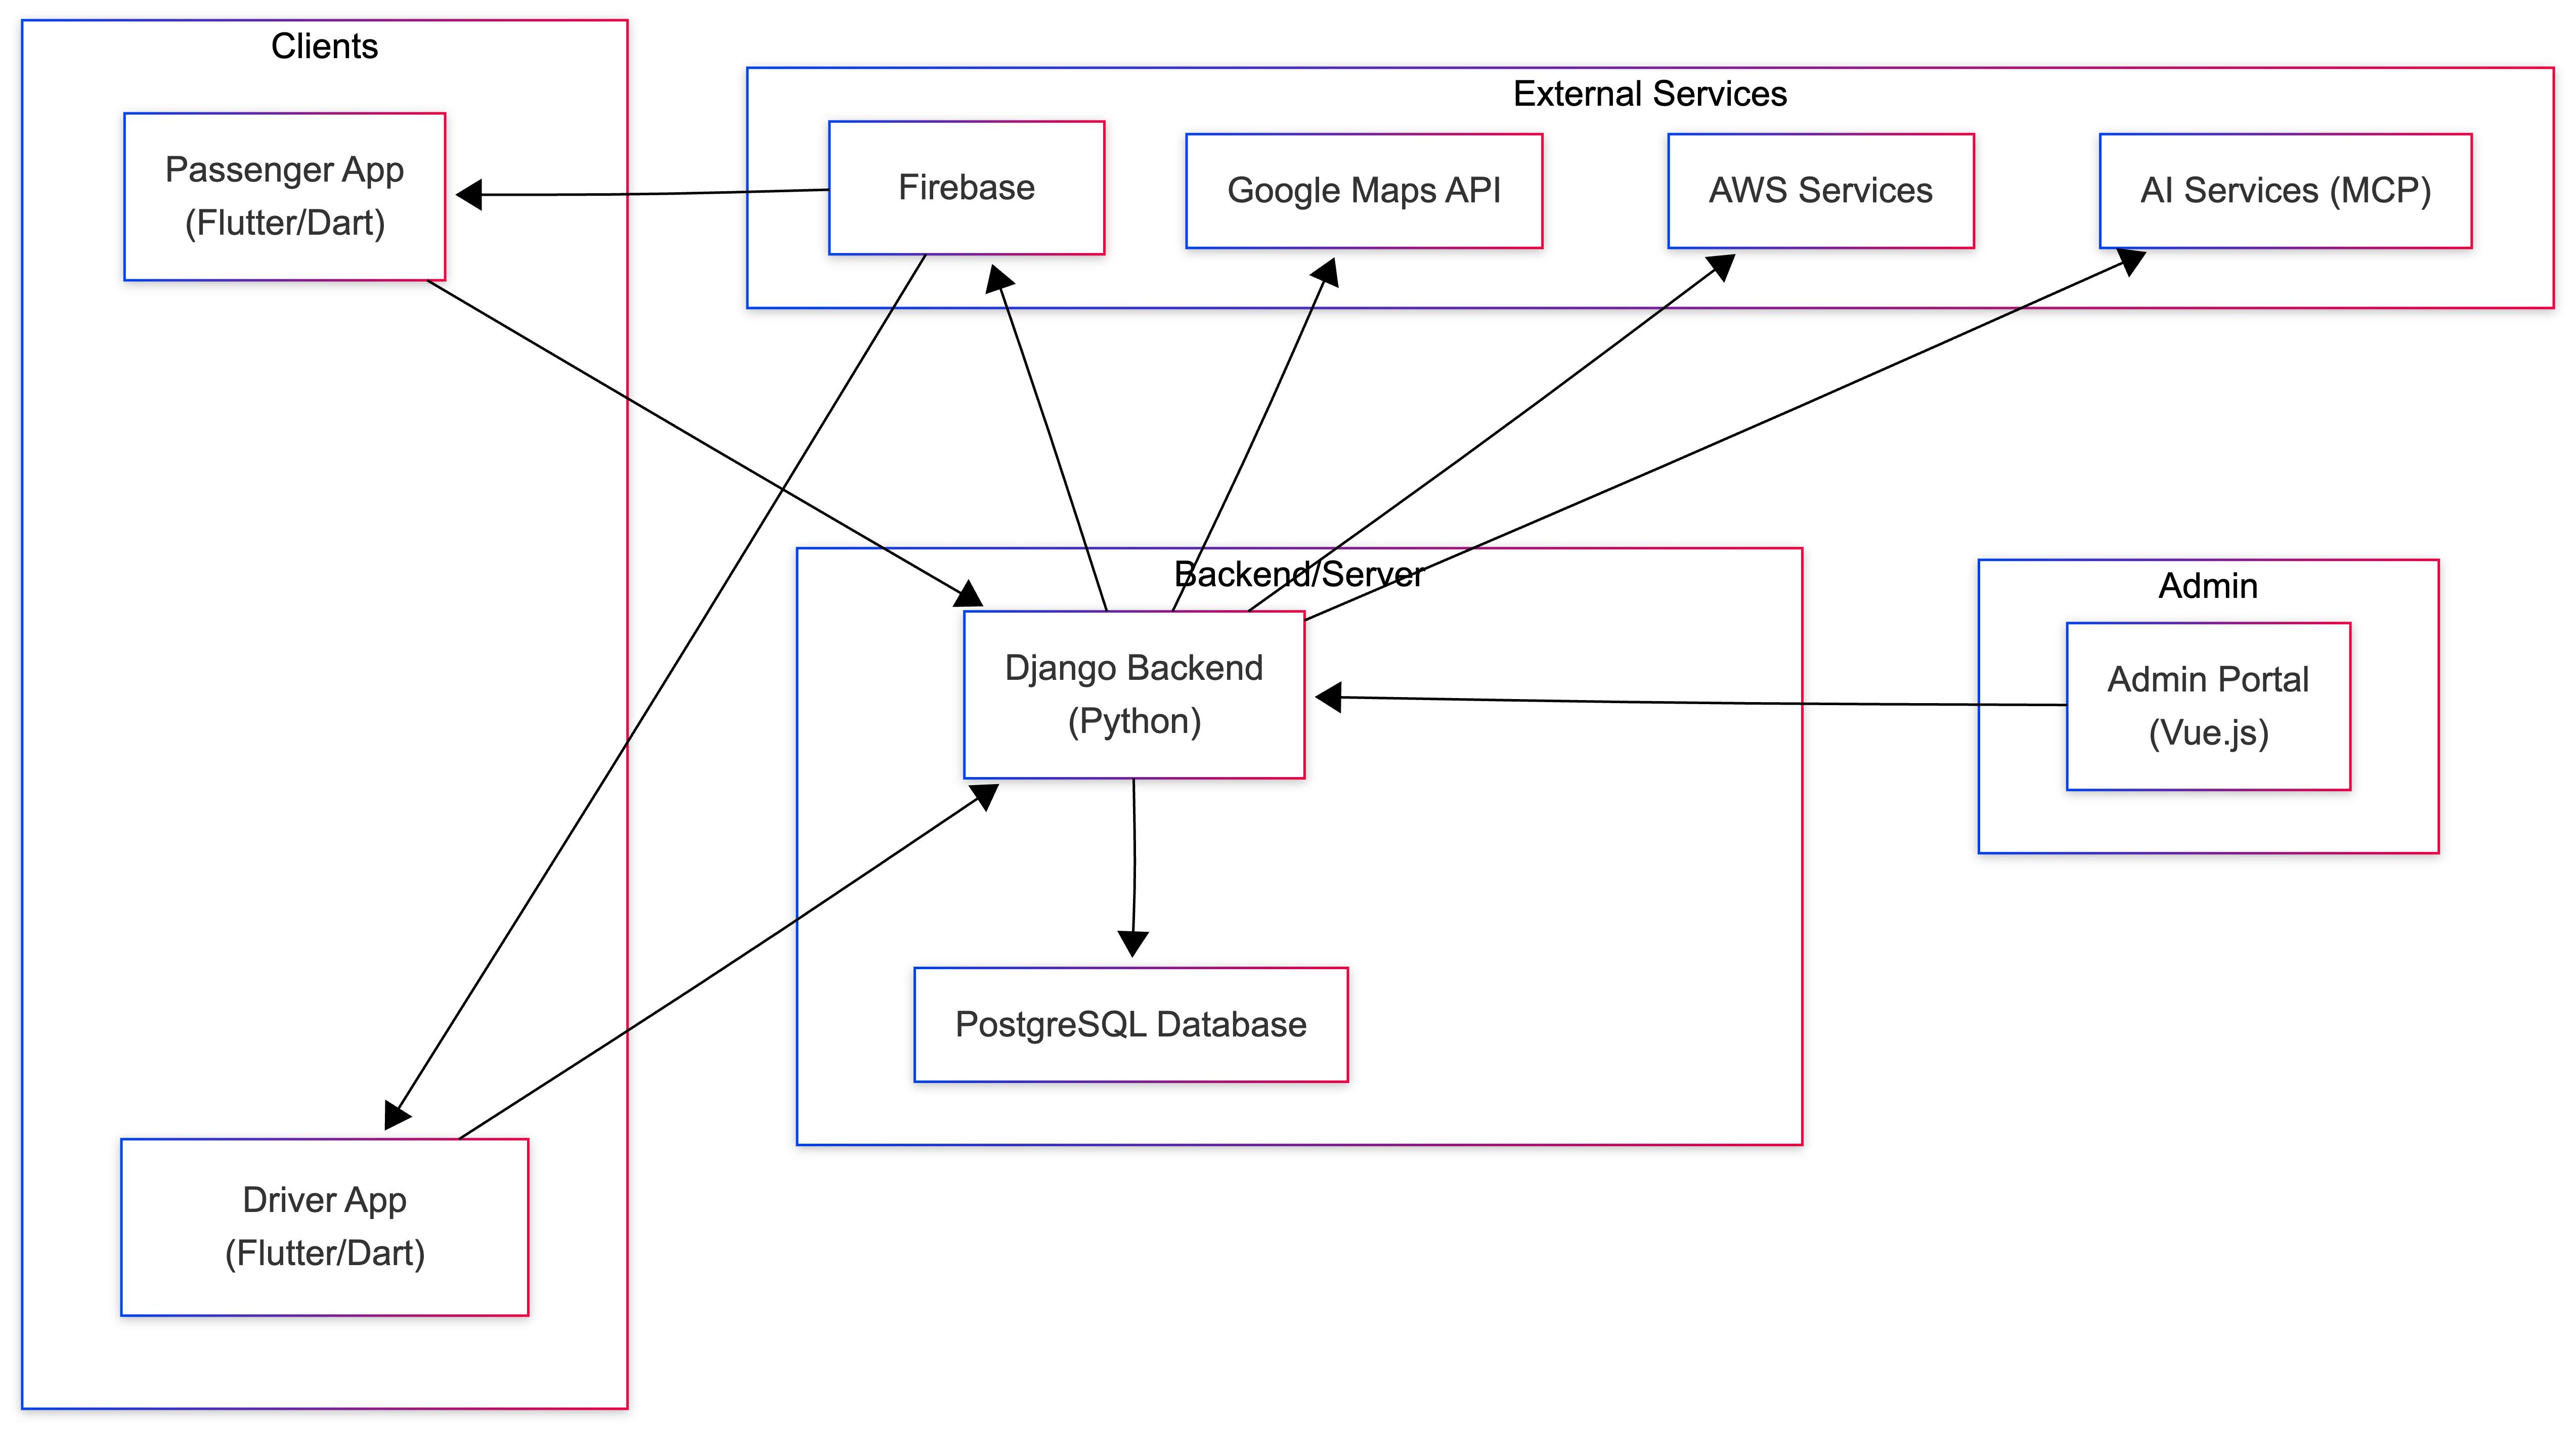
\includegraphics[width=0.8\textwidth]{images/methodology_2.png}
\caption{Methodology diagram of the entire system flow}
\label{fig:methodology}
\end{figure}

\subsection{Implementation}

The Traxis system was developed using an Agile-inspired iterative approach, structured around three focused sprints of approximately 3–4 weeks each. This methodology ensured continuous feedback, early delivery of functional components, and adaptability to evolving requirements. Development of the Passenger and Driver applications was performed from a single Flutter codebase, guaranteeing 100\% feature parity and identical behavior on both Android and iOS platforms from the outset.

\begin{itemize}
    \item \textbf{Sprint 1 – Foundation (Weeks 1–4)} \\
          The first sprint established the core infrastructure of the system. This included:
          \begin{itemize}
              \item Backend scaffolding with \textbf{Django} and \textbf{Django REST Framework}, creating the initial API endpoints and authentication logic.
              \item Database setup with \textbf{PostgreSQL} and the \textbf{PostGIS} extension, supporting geospatial queries for future ride matching and route calculations.
              \item Integration of \textbf{Firebase Authentication} for secure phone-number-based login and \textbf{Cloud Messaging} for real-time notifications.
              \item Implementation of the real-time location pipeline to track passenger and driver positions efficiently.
              \item Initial setup of \textbf{MCP (Model Control Plane)} for AI service integration, preparing APIs for future predictive ride matching and AI-based recommendations.
              \item Configuration of \textbf{AWS services} for compute-intensive tasks such as transcription, batch processing, and AI computations.
          \end{itemize}

    \item \textbf{Sprint 2 – Core Interaction (Weeks 5–8)} \\
          The second sprint focused on user-facing functionality and real-time interactions:
          \begin{itemize}
              \item Development of \textbf{Passenger and Driver UI components} using Flutter, including ride request flows, driver availability status, and passenger booking screens.
              \item Implementation of phone-number login with OTP verification, leveraging Firebase Authentication.
              \item Driver availability broadcasting and passenger request handling via the backend and Firebase Cloud Messaging.
              \item Aggressive local caching using \textbf{Hive} to maintain functionality in low-connectivity or intermittent network areas.
              \item Real-time push notifications for ride status updates and driver-passenger communication.
              \item Integration of MCP-based AI features into core flows, including predictive driver matching and demand forecasting, communicating via backend APIs.
              \item Offloading heavy processing tasks to AWS services, such as voice-to-text transcription for ride requests.
          \end{itemize}

    \item \textbf{Sprint 3 – Polish \& Advanced Features (Weeks 9–12)} \\
          The third sprint added advanced features, optimization, and system polish:
          \begin{itemize}
              \item Heatmap visualization for demand prediction and operational insights, leveraging MCP AI analytics.
              \item Trip history and detailed ride analytics for passengers and drivers.
              \item Rating and feedback system to ensure service quality.
              \item Admin portal enhancements, including dispute resolution tools and reporting dashboards.
              \item Performance tuning for backend and mobile apps, including optimization of AWS-backed compute tasks and MCP API calls.
              \item Accessibility features, such as voice prompts for drivers, high-contrast UI modes, and intuitive navigation.
          \end{itemize}
\end{itemize}

This implementation plan ensured that core functionality was delivered early, enabling iterative testing and feedback while progressively integrating advanced AI features and cloud-based services. By following this structured Agile approach, the development team maintained high code quality, ensured system reliability, and supported rapid adaptation to emerging user and business needs.

\begin{figure}[h]
\centering
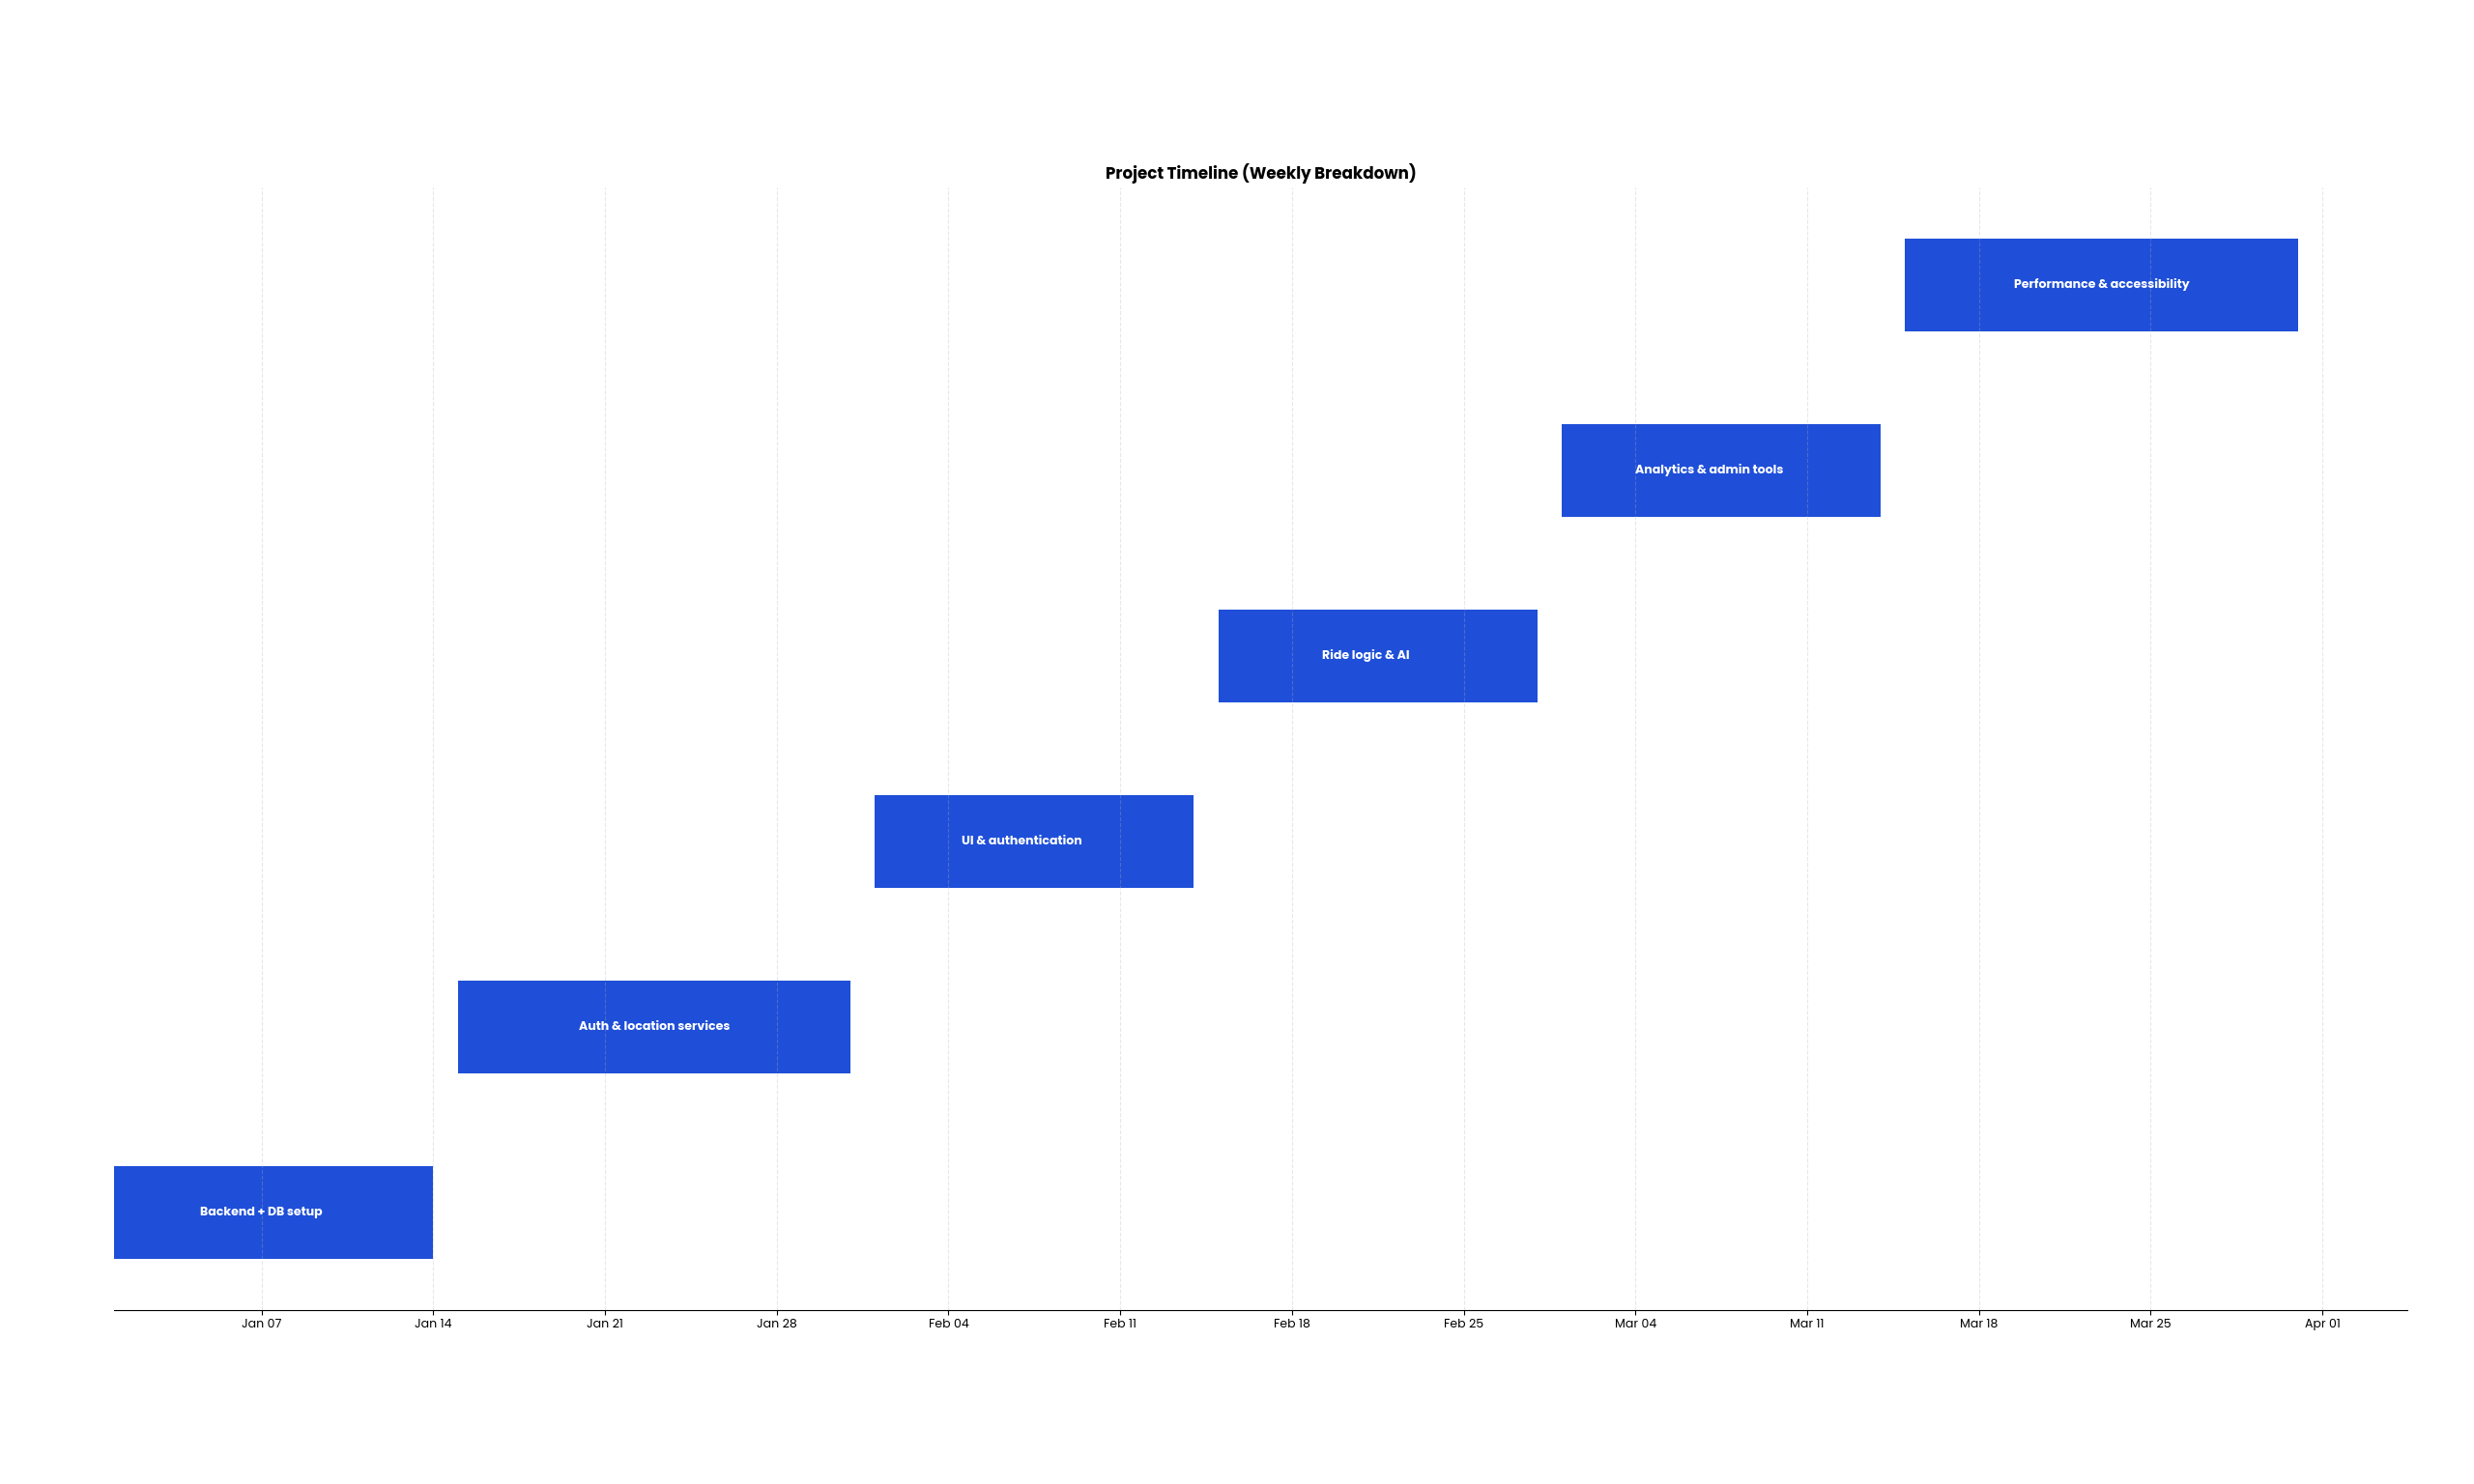
\includegraphics[width=1.05\textwidth]{images/gantt_2.png}
\caption{Gantt Chart showing the intended work plan}
\label{fig:gantt}
\end{figure}


\subsection{Project Management \& Version Control}

\textbf{Version Control: GitHub} \\
The project utilized GitHub for source code management and version control. A structured branching strategy was employed, including a \texttt{main} branch for production-ready code and a \texttt{develop} branch for ongoing development. All feature additions, bug fixes, and improvements were implemented through pull requests (PRs), which underwent code review before merging. This approach ensured code quality, traceability, and collaborative development while minimizing integration errors.

\textbf{Project Management: ClickUp} \\
ClickUp was used to plan, track, and manage all project activities. The platform supported the Agile sprint structure with task assignments, deadlines, and progress tracking through burndown charts. Automated reminders and notifications helped prevent task slippage, ensuring timely completion of features and alignment with the overall project timeline. Additionally, ClickUp provided transparency and accountability for all team members, facilitating efficient communication and coordination throughout the project lifecycle.

\chapter{System Analysis and Design}
\label{chap:system_analysis_design}

This chapter describes the system study, analysis and design of the system. It highlights the identified requirements and the architectural design of the system.

\section{System Study}

The study was carried out on Hills Link Express, a private shuttle service operating seven- and fourteen-seater vans along the Kampala--Kabale route. The primary objective was to understand how the private shuttle transport system currently operates and to identify the specific inefficiencies that a digital solution could address.

Findings revealed that the system in use is largely manual and heavily dependent on informal processes. To book a ride, prospective passengers are required to contact the shuttle operator via phone calls. As a result, the business owner relies on multiple phones to handle and manage booking requests simultaneously. Booking confirmation is also conducted manually; payments are typically made in cash, and in cases where customers use digital platforms such as MTN MoMo Pay, the operator takes a photo of the transaction receipt and sends it to the customer as proof of payment. This approach is inefficient, unstructured, and difficult to manage, particularly as demand increases.

Further analysis of the system revealed several key operational challenges, which are discussed below.

\begin{itemize}

    \item \textbf{Lack of a structured booking process:} The booking process lacks structure and accountability. Customers are able to reserve seats but may fail to show up without prior cancellation or communication. This results in revenue loss and underutilised seats. Additionally, the reliance on phone-based communication places a significant burden on the operator, who must continuously respond to booking enquiries, location updates, and delivery status requests. This form of communication is not scalable and becomes increasingly difficult to manage as the customer base grows.

    \item \textbf{Unreliable seat allocation and poor seat utilisation:} The current system does not provide a transparent or reliable mechanism for seat allocation. Although passengers may request specific seats, such as front seats, these requests are not guaranteed, as operators may reassign seats based on personal preferences or customer relationships. This creates a lack of trust and transparency in the booking process. In addition, seat utilisation is inefficient. Passengers may disembark at intermediate locations such as Mbarara, leaving empty seats that are not reassigned for the remainder of the journey. The absence of a system to dynamically match available seats with passengers along the route leads to missed revenue opportunities and reduced operational efficiency.

    \item \textbf{Limited service visibility and discoverability:} The service relies primarily on word-of-mouth referrals and radio advertisements, making it difficult for new customers to discover and access the service. This limits the business's reach and growth potential. Additionally, there is no centralised platform where customers can view available routes, schedules, or pricing information. Accessibility is further affected by varying levels of digital literacy among users. While some customers may prefer digital solutions, others rely on phone calls, highlighting the need for a system that accommodates both interaction methods.

    \item \textbf{Absence of parcel tracking:} The shuttle service also handles parcel delivery; however, there is no system for tracking shipments in real time. Customers frequently contact the operator to enquire about the status and location of their goods, increasing the communication burden. In addition, there is no structured approach to managing the balance between passenger transport and cargo. Vehicles may carry either passengers or goods depending on demand, but without a system to optimise this allocation, potential efficiency gains are lost.

    \item \textbf{Limited operational visibility for the business owner:} The current system provides limited visibility for the business owner. It is difficult to track vehicle movement, monitor driver activity, verify reported revenue, or determine seat occupancy in real time. This lack of operational insight reduces the owner's ability to make informed decisions and effectively manage the business. Return trips present an additional challenge, as demand is often low. Without visibility into passenger demand, drivers may remain at the destination rather than returning, leading to inefficiencies in service utilisation.

    \item \textbf{Lack of passenger accountability and safety records:} The system lacks structured mechanisms for tracking passengers and ensuring accountability. There is no reliable record of who was on a vehicle, where passengers boarded or disembarked, or emergency contact information. This creates potential safety risks and limits the ability to respond effectively in case of incidents.

\end{itemize}

\section{System Analysis}

\subsection{Data Analysis and Interpretation of Results}

The findings from the system study reveal that the current private shuttle transport system is largely informal, unstructured, and inefficient in handling core operational processes. The heavy reliance on manual and phone-based interactions limits the scalability of the service and increases the likelihood of errors, miscommunication, and operational delays.

A key issue identified is the lack of a structured booking system, which results in unreliable seat reservations and frequent no-shows. This directly affects revenue generation and reduces overall efficiency. In addition, the absence of real-time seat management prevents the system from reallocating seats when passengers disembark mid-journey, leading to underutilisation of available capacity.

Communication within the system is also inefficient, as the operator is required to handle all customer interactions manually. This creates bottlenecks and limits the ability of the business to expand. Similarly, the lack of service visibility restricts customer access, as potential users have no easy way to discover routes, schedules, or availability.

From a logistics perspective, the absence of a tracking system for both passengers and parcels results in constant enquiries and increased workload for the operator. Furthermore, the inability to balance passenger and cargo transport reduces operational optimisation opportunities.

The analysis also highlights limited operational control and visibility for the business owner. Without real-time monitoring of vehicles, revenue, and occupancy, it is difficult to make informed decisions or verify driver activity. Safety concerns are also evident due to the lack of structured passenger records and traceability mechanisms.

Overall, the current system demonstrates significant gaps in coordination, transparency, and efficiency. These findings justify the need for a digital solution that can automate booking, improve communication, enable real-time tracking, and provide better operational control.

\subsection{User Requirements}

The following are the requirements the users expect Traxis to meet:

\begin{enumerate}
    \item Users need a simple way to book shuttle seats without making phone calls.
    \item Passengers need the ability to select specific seats.
    \item Users require confirmation after making a booking or payment.
    \item Passengers need to know shuttle location and arrival times.
    \item Customers need a way to track parcels during delivery.
    \item Operators need a way to monitor vehicle movement and seat occupancy.
    \item The system should reduce excessive phone communication.
    \item The system should be easy to use for individuals with low digital literacy.
\end{enumerate}

\subsection{Functional Requirements}

The system was required to provide the following core functionalities:

\begin{enumerate}
    \item Allow passengers to create accounts using phone numbers.
    \item Enable users to search for available shuttle routes and schedules.
    \item Allow passengers to book specific seats on a shuttle.
    \item Provide real-time updates on seat availability.
    \item Enable passengers to make payments and receive automated confirmation.
    \item Allow users to cancel bookings based on defined conditions.
    \item Provide real-time tracking of shuttle location.
    \item Enable passengers to receive notifications on trip status and updates.
    \item Allow operators to manage bookings and update seat availability.
    \item Enable operators to monitor vehicle movement in real time.
    \item Provide a dashboard for viewing revenue, trips, and occupancy levels.
    \item Allow operators to update passenger and trip records.
    \item Support courier service functionality, including:
        \begin{itemize}
            \item Recording parcel details
            \item Tracking delivery status
            \item Notifying users upon delivery
        \end{itemize}
    \item Provide a hybrid communication system that supports both in-app interaction and phone-based contact.
\end{enumerate}

\subsection{Non-Functional Requirements}

The system was designed to be user-friendly and accessible to individuals with varying levels of digital literacy. It should:

\begin{enumerate}
    \item Allow users to access system features immediately after successful authentication.
    \item Provide a simple and intuitive interface for easy navigation between different sections of the application.
    \item Minimise user input errors through validation mechanisms.
    \item Allow users to easily correct input errors before submission.
    \item Provide clear feedback and notifications upon successful completion of key actions such as registration, booking, and payment.
    \item Assure fluid UI animations (e.g. consistent 400ms page transitions) to maintain a premium end-user experience.
    \item Efficiently handle peak traffic times, such as holiday seasons, without failing to process transactions or generate digital tickets.
    \item Transmit personal user data, location details, and payment information securely using modern encryption standards.
\end{enumerate}

\subsection{System Requirements}

\begin{itemize}
    \item \textbf{Platform Compatibility:} The application must be compatible with Android 8.0 (API level 26) and above, as well as iOS 12.0 and above.
    \item \textbf{Network Connectivity:} An active internet connection (3G/4G/5G or Wi-Fi) is required for real-time synchronisation of location data, bookings, and notifications.
    \item \textbf{Hardware:} A standard mobile device equipped with location service capabilities (GPS) and a minimum of 2\,GB RAM.
\end{itemize}

\section{System Design}

This section includes a detailed description of the system's architecture, components, modules, interfaces, and data structures designed to satisfy the specified requirements. It describes the design and development process of the application using a use case diagram to explain how actors interact with the system and data flow diagrams to show how data moves in and out of the system.

\subsection{System Architecture}

TRAXIS employs a \textbf{Client-Server Architecture} built on a layered, modular design pattern. The Flutter application serves as the client interface, responsible for UI rendering, state management, and local caching, while a centralised cloud-hosted backend acts as the single source of truth for all data and business logic.

The architecture is divided into four principal layers:

\begin{enumerate}
    \item \textbf{Presentation Layer:} Encompasses all interactive Flutter screens (e.g., \texttt{dashboard\_screen}, \texttt{operator\_dashboard\_screen}, \texttt{digital\_ticket\_screen}) and UI widgets using dynamic layouts and global theming defined in \texttt{app\_theme.dart}.

    \item \textbf{Core / Domain Layer:} Houses the business logic, utilising providers (e.g., \texttt{auth\_provider.dart}) and state management mechanisms to bridge the data and presentation layers.

    \item \textbf{Data Layer:} Manages API integrations, external service calls, and secure local storage mechanisms, ensuring clean separation between business logic and data access.

    \item \textbf{External Services Layer:} Integrates third-party services including Firebase (authentication, messaging, real-time sync), Google Maps API (geolocation and routing), AWS Services (compute-intensive tasks), and AI services via MCP.
\end{enumerate}

\subsubsection{Use Case Diagram}

The use case diagram below illustrates the different types of users of the system and how they interact with it. Two primary actors are identified: the \textbf{Passenger} and the \textbf{Operator}. The diagram provides a simplified graphical representation of the system's functionalities and the interactions each actor may perform.

\begin{figure}[h]
\centering

\includegraphics[width=0.85\textwidth]{images/FYP/fig41_usecase_diagram.png}
\caption{Use case diagram showing how users interact with the Traxis system}
\label{fig:use_case}
\end{figure}

\subsubsection{Context Diagrams}

A context diagram describes the logical flow of data within the system, illustrating how each user type interacts with the system from authentication through to completing their primary tasks. The Level 0 diagram below presents the system as a single process, showing all external entities and their data exchanges with the system.

\begin{figure}[h]
\centering

\includegraphics[width=0.80\textwidth]{images/FYP/fig42_level0_context.png}
\caption{Level 0 Context Diagram showing the overall system boundary and external entities}
\label{fig:context_l0}
\end{figure}

The Level 1 diagram decomposes the system further, revealing the core internal processes, data stores, and information flows between passengers, operators, and the Traxis platform.

\begin{figure}[h]
\centering
\includegraphics[width=0.85\textwidth]{images/FYP/fig43_level1_context.png}
\caption{Level 1 Context Diagram showing internal processes and data flows}
\label{fig:context_l1}
\end{figure}

\subsection{Design Constraints}

\begin{itemize}
    \item \textbf{Cross-Platform Consistency:} Maintaining a uniform graphical experience across both iOS and Android natively while avoiding UI inconsistencies between the two platforms.
    \item \textbf{Network Dependency:} Real-time tracking and live ticketing mandate continuous internet and GPS connectivity. The system must gracefully handle offline or low-connectivity degradation, using local caching via Hive to queue actions until connectivity is restored.
    \item \textbf{Mobile Hardware Limitations:} Rendering complex UI animations (ambient blur orbs, gradients) and active map overlays requires meticulous memory optimisation to prevent frame rate drops or device overheating, particularly on low- and mid-range devices common in Uganda.
    \item \textbf{Internet Connectivity Requirement:} All location server platforms implemented require active internet connectivity for real-time synchronisation. The response time for location data is therefore dependent on the quality of the mobile network available to the user.
\end{itemize}

\subsection{Design Methodology}

We used the \textbf{Agile development methodology}. Agile Software Development (ASD) is a creative process that anticipates the need for flexibility and applies a high level of pragmatism into the delivery of the finished product. We focused on keeping code simple, testing often, and delivering functional components of the application as soon as they were ready. This helped us to minimise risks such as bugs, cost overruns, and changing requirements. Rapid prototyping of the graphical user interface was conducted first to gather immediate feedback on custom aesthetic elements. Following approval of the UI design, functional milestones were iteratively coded and deployed, linking the distinct passenger and operator workflows in sequential project sprints.

\subsection{High Level Design}

The high-level design structures the application into self-contained major subsystems:

\begin{enumerate}
    \item \textbf{Identity and Access Management:} OTP issuance, user profile creation, role retrieval, and session token management.
    \item \textbf{Passenger Operations Subsystem:} A pipeline covering: Search $\rightarrow$ Seat Selection $\rightarrow$ Payment $\rightarrow$ Digital Ticketing.
    \item \textbf{Logistics and Tracking Subsystem:} Real-time vehicle geolocation and package dispatch tracking using mapping services.
    \item \textbf{Operator Management Subsystem:} Dedicated to dashboard rendering, booking aggregation, and financial analytics.
\end{enumerate}

\subsubsection{Conceptual or Logical Design}

This view shows the logical functional elements of the system, clearly indicating the major processes involved and how they relate to one another.

At a logical level, the system separates actions driven by user roles that interact with shared data entities:

\begin{itemize}
    \item \textbf{Entities:} Users, Trips, Bookings, Tickets, Packages, and Transport Vehicles.
    \item A \textit{Passenger} interacts with the system to create multiple Bookings and package requests.
    \item A \textit{Booking} generates exactly one Digital Ticket and links a User to a specific Seat on a scheduled Trip.
    \item An \textit{Operator} orchestrates Trips and views aggregated metadata spanning numerous Bookings.
\end{itemize}

\subsubsection{Process (Module) Design}

This view is for project management and code organisation. The components are organised as independent modules corresponding to files or directories within the codebase. The primary functional modules implemented within the TRAXIS codebase include:

\begin{itemize}
    \item \textbf{Authentication Module:} Manages the entry threshold securely through Role Selection and OTP Verification screens.
    \item \textbf{Customer Module:} Features route planning, interactive seat mapping, and generation of the boarding pass (\texttt{search\_booking\_screen}, \texttt{seat\_selection\_screen}, \texttt{digital\_ticket\_screen}).
    \item \textbf{Operator Module:} Fetches enterprise-level metrics to render bookings and financial revenue on specialised dashboards (\texttt{operator\_dashboard\_screen}, \texttt{operator\_bookings\_screen}).
    \item \textbf{Tracking and Delivery Module:} Interfaces with map SDKs to parse and display real-time coordinate updates for vehicles (\texttt{live\_tracking\_screen}, \texttt{package\_delivery\_screen}).
\end{itemize}

\begin{figure}[h]
\centering
\includegraphics[width=0.80\textwidth]{images/FYP/fig44_module_structure.png}
\caption{Directory structure of the build and development environment}
\label{fig:module}
\end{figure}

\subsubsection{Security}

Traxis enforces security at multiple levels. Authentication is handled exclusively through OTP-based phone number verification via Firebase Authentication, eliminating password-related vulnerabilities. All external communication operates strictly over HTTPS protocols. Sensitive user data, location details, and payment information are transmitted using modern encryption standards. Role-based access control ensures that passengers and operators can only access functionality appropriate to their role, with role retrieval and session token management handled by the Core/Domain layer through \texttt{auth\_provider.dart}.

\subsection{Database Design}

Operating via scalable, cloud-based data structures (Cloud Firestore and PostgreSQL), the core relations are organised as follows:

\begin{itemize}
    \item \textbf{Users:} \texttt{user\_id}, \texttt{role\_type} (customer vs. operator), \texttt{phone\_number}, \texttt{profile\_metadata}.
    \item \textbf{Trips / Routes:} \texttt{trip\_id}, \texttt{operator\_id}, \texttt{departure\_location}, \texttt{destination\_location}, \texttt{schedule\_time}, \texttt{vehicle\_id}.
    \item \textbf{Bookings:} \texttt{booking\_id}, \texttt{user\_id}, \texttt{trip\_id}, \texttt{seat\_numbers}, \texttt{transaction\_amount}, \texttt{payment\_status}.
    \item \textbf{Packages:} \texttt{package\_id}, \texttt{sender\_id}, \texttt{receiver\_info}, \texttt{assigned\_trip\_id}, \texttt{delivery\_status}.
\end{itemize}

\subsubsection{Adding Data}

Data is written to the backend through RESTful API endpoints exposed by the Django REST Framework. For real-time features, data is simultaneously synchronised to Cloud Firestore using the Firebase SDK. Each record is identified by a unique ID generated at the point of creation. For example, when a passenger confirms a booking, a \texttt{booking\_id} is generated, the corresponding seat record is updated to reflect occupancy, and a digital ticket entry is created — all within a single transactional API call to ensure data consistency.

\subsubsection{Reading Data}

Data is retrieved from the backend via RESTful API calls authenticated using session tokens. For real-time features such as live vehicle tracking and seat availability updates, the application subscribes to Firestore document streams. Changes to tracked documents (e.g. a vehicle's GPS coordinates or a seat's occupancy status) are pushed to all connected clients sub-second, ensuring that every passenger and operator always sees the most current system state.

\subsection{GUI Design}

\subsubsection{Inputs}

\begin{itemize}
    \item \textbf{Phone number and OTP:} Required on registration and login. Without valid credentials, a user cannot authenticate or access any system functionality.
    \item \textbf{GPS coordinates:} The application requests location permission from the device. This allows the user's position and the vehicle's position to be determined and displayed in real time.
    \item \textbf{Seat selection taps:} Passengers interact with an interactive seat grid to choose their preferred seat. The grid reflects real-time availability, with occupied seats visually distinguished from available ones.
    \item \textbf{Booking and payment details:} Users input trip preferences and payment information through validated form fields, with inline error messages displayed immediately upon detection of invalid input.
    \item \textbf{Package details:} For courier requests, users provide sender and receiver information, which is stored against the assigned trip.
\end{itemize}

\subsubsection{Outputs}

\begin{itemize}
    \item \textbf{Interactive map view:} Immediately upon authentication, both passengers and operators are presented with a live map view (powered by Google Maps SDK) showing real-time vehicle positions.
    \item \textbf{Digital ticket:} Upon successful payment, the system generates and displays a digital boarding pass (\texttt{digital\_ticket\_screen}) containing booking reference, seat number, route, and departure time.
    \item \textbf{Status notifications:} Push notifications via Firebase Cloud Messaging alert passengers to trip status changes, payment confirmations, and parcel delivery updates.
    \item \textbf{Operator dashboard:} A 2$\times$2 KPI grid displays live metrics including active bookings, revenue generated, seat occupancy rate, and active trips.
    \item \textbf{Ride history and booking lists:} Scrollable list views (\texttt{ride\_history\_screen}, \texttt{operator\_bookings\_screen}) present historical and current booking records with clear visual and tactile feedback for all system states.
\end{itemize}

\subsection{External Interfaces}

\subsubsection{Hardware Interfaces}

\begin{itemize}
    \item \textbf{Geospatial Sensors:} The application calls the device's native GPS unit to continuously fetch and render user and transport locations. The \texttt{ACCESS\_FINE\_LOCATION} permission is declared in the application manifest, and users must grant this permission for full tracking functionality.
    \item \textbf{Haptic Interfaces:} Device vibration motors are engaged on key user interactions such as seat selections or payment verifications, providing tactile confirmation of actions.
\end{itemize}

\subsubsection{Software Interfaces}

\begin{itemize}
    \item \textbf{Device OS Integrations:} Deep interaction with the Android SDK and iOS Foundation frameworks is required to retrieve hardware permissions for location services and push notifications.
    \item \textbf{Mapping APIs:} Integration with the Google Maps SDK provides route polyline rendering and live vehicle tracking overlays. OpenStreetMap tiles are cached locally as a fallback for low-connectivity environments.
\end{itemize}

\subsubsection{Communication Interfaces}

\begin{itemize}
    \item \textbf{RESTful JSON APIs:} All client-to-server communication operates strictly over HTTPS, with JSON as the data exchange format. API endpoints are managed by the Django REST Framework.
    \item \textbf{WebSockets / Firestore Streams:} Low-latency, bi-directional data streams via Firestore maintain the persistent real-time functionality required by the live location tracking and seat availability modules, ensuring sub-second updates even on 3G networks.
    \item \textbf{Firebase Cloud Messaging (FCM):} Push notifications for ride status updates, booking confirmations, and parcel delivery alerts are delivered to both passenger and operator devices through FCM without requiring custom notification infrastructure.
\end{itemize}

\subsubsection{User Interfaces}

The user-facing platform consists of dynamic, touch-responsive screens built with the Flutter framework. Core aesthetic elements include custom modern typography, a tailored colour palette featuring vibrant interactive gradients, and specialised glassmorphic overlays (blur orbs, translucent card panels). Navigation is provided through a carved-out bottom navigation bar with clear active/inactive visual states. Transition animations between application states are set to an optimal 400\,ms duration, prioritising fluidity over abrupt page loads. Integral interactive elements include OTP \texttt{TextFields}, responsive map layouts, and dynamic seating grids. The interface adopts \textbf{distinct dashboard layouts} for Operators (emphasising KPIs and operational data) and Passengers (emphasising action buttons, interactive maps, and ticketing) while rigorously adhering to a globally unified theme defined in \texttt{app\_theme.dart}.
\chapter{System Implementation, Testing and Validation}

\section{Introduction}
This chapter describes how Traxis was realized. Traxis's implementation, testing and validation was to make sure that it meets its set
objectives and the requirement specifications that were identified.

\section{System Implementation}
This section gives an overview of the project implementation. It highlights
the major components and the operation of the system as well as the different
user interfaces and activities that allow users to interact with the system.

\subsection{Implementation tools}
The Traxis system was implemented using a modern, scalable technology stack selected to ensure performance, reliability, and adaptability within the Ugandan transport context.

\textbf{Flutter (Dart)}
The mobile application was developed using Flutter, a cross-platform UI framework by Google, alongside the Dart programming language. Flutter enabled the development of a single codebase that runs on both Android and iOS devices, reducing development time and maintenance effort. Its widget-based architecture supported the creation of responsive and user-friendly interfaces suitable for a wide range of devices, including low and mid-range smartphones commonly used in Uganda.

\textbf{Django and Django REST Framework (DRF)}
The backend system was implemented using Django, a high-level Python web framework, together with the Django REST Framework for API development. Django handled business logic, request processing, and system coordination, while DRF exposed RESTful APIs that facilitated secure communication between the mobile applications, admin portal, and external services.

\textbf{PostgreSQL (with PostGIS)}
PostgreSQL was used as the primary relational database for persistent data storage. It provided strong data integrity, reliability, and support for complex queries. The PostGIS extension enabled geospatial data processing, which was essential for location-based features such as route mapping, nearest-vehicle identification, and geographic queries.

\textbf{Firebase Services}
Firebase was integrated to support real-time features and user management:

Firebase Authentication was used for secure user registration and login, particularly through phone-number-based authentication, which aligns with local user accessibility.
Firebase Cloud Messaging (FCM) enabled real-time push notifications, such as booking confirmations, trip updates, and alerts for both passengers and drivers.

\textbf{Google Maps API}
The Google Maps Platform was used to provide mapping, navigation, and geolocation services. It enabled real-time vehicle tracking, route visualization, and distance calculations, improving user interaction and operational coordination within the system.

\textbf{AWS (Amazon Web Services)}
AWS was utilized for compute-intensive operations such as transcription and other backend processing tasks. Its scalable cloud infrastructure ensured efficient handling of resource-demanding processes without affecting overall system performance.

\textbf{MCP (Model Control Protocol)}
MCP was integrated to support AI-driven functionalities, including predictive analytics and intelligent system behavior. Implemented using Python, it enabled advanced features such as demand forecasting and improved coordination between passengers and shuttle operators.

\textbf{Hive and Background Sync Mechanisms}
Hive, a lightweight local database for Flutter, was used to support offline functionality. Combined with background synchronization tools, it allowed the system to queue actions performed offline and automatically sync them once network connectivity was restored—an essential feature for areas with unstable internet access.

\textbf{Vue.js (Admin Portal)}
The Admin Portal was developed using Vue.js, a progressive JavaScript framework. It provided administrators with a responsive interface for managing users, monitoring trips, viewing analytics, and configuring system settings. Its reactive architecture enabled real-time updates and efficient interaction with backend APIs.

\subsection{User interface design}
The system can be launched from the phone just like any other Android or IOS
applications and after it has been launched, a login interface appears. This
is helpful in authenticating users
\subsubsection{Account Creation}
Passengers can create an account by providing their phone number and a next of kin's phone number, which is verified through a one-time password (OTP) sent via SMS. Operators are asked to provide an E-mail address in addition to their phone number. This method ensures a secure and straightforward registration process, particularly suited for users in Uganda who may not have access to email-based authentication.

\subsubsection{Operator Actions}
Once logged in, operators can access the main dashboard, which provides options for booking rides, viewing trip history, and managing their profiles. The interface is designed to be intuitive and user-friendly, with clear navigation and accessible features. Operators can register a company, the number of vehicles they have,the routes they operate on, and how much they charge for specific routes. They can also view and manage their bookings and indicate whether or not they support parcel delivery. On the dashboard, they can also view the number of passengers that have booked rides with them and the total revenue earned. They can add new vehicles to their fleet and view the details of their vehicles such as their location during trips and the number of trips they have made. Operators can also view the details of their passengers such as their name, phone number, and next of kin's phone number. They can also view the details of their trips such as the route taken, the distance covered, and the fare charged. 

\begin{figure}[htbp]
\centering

\begin{subfigure}{0.32\textwidth}
    \centering
    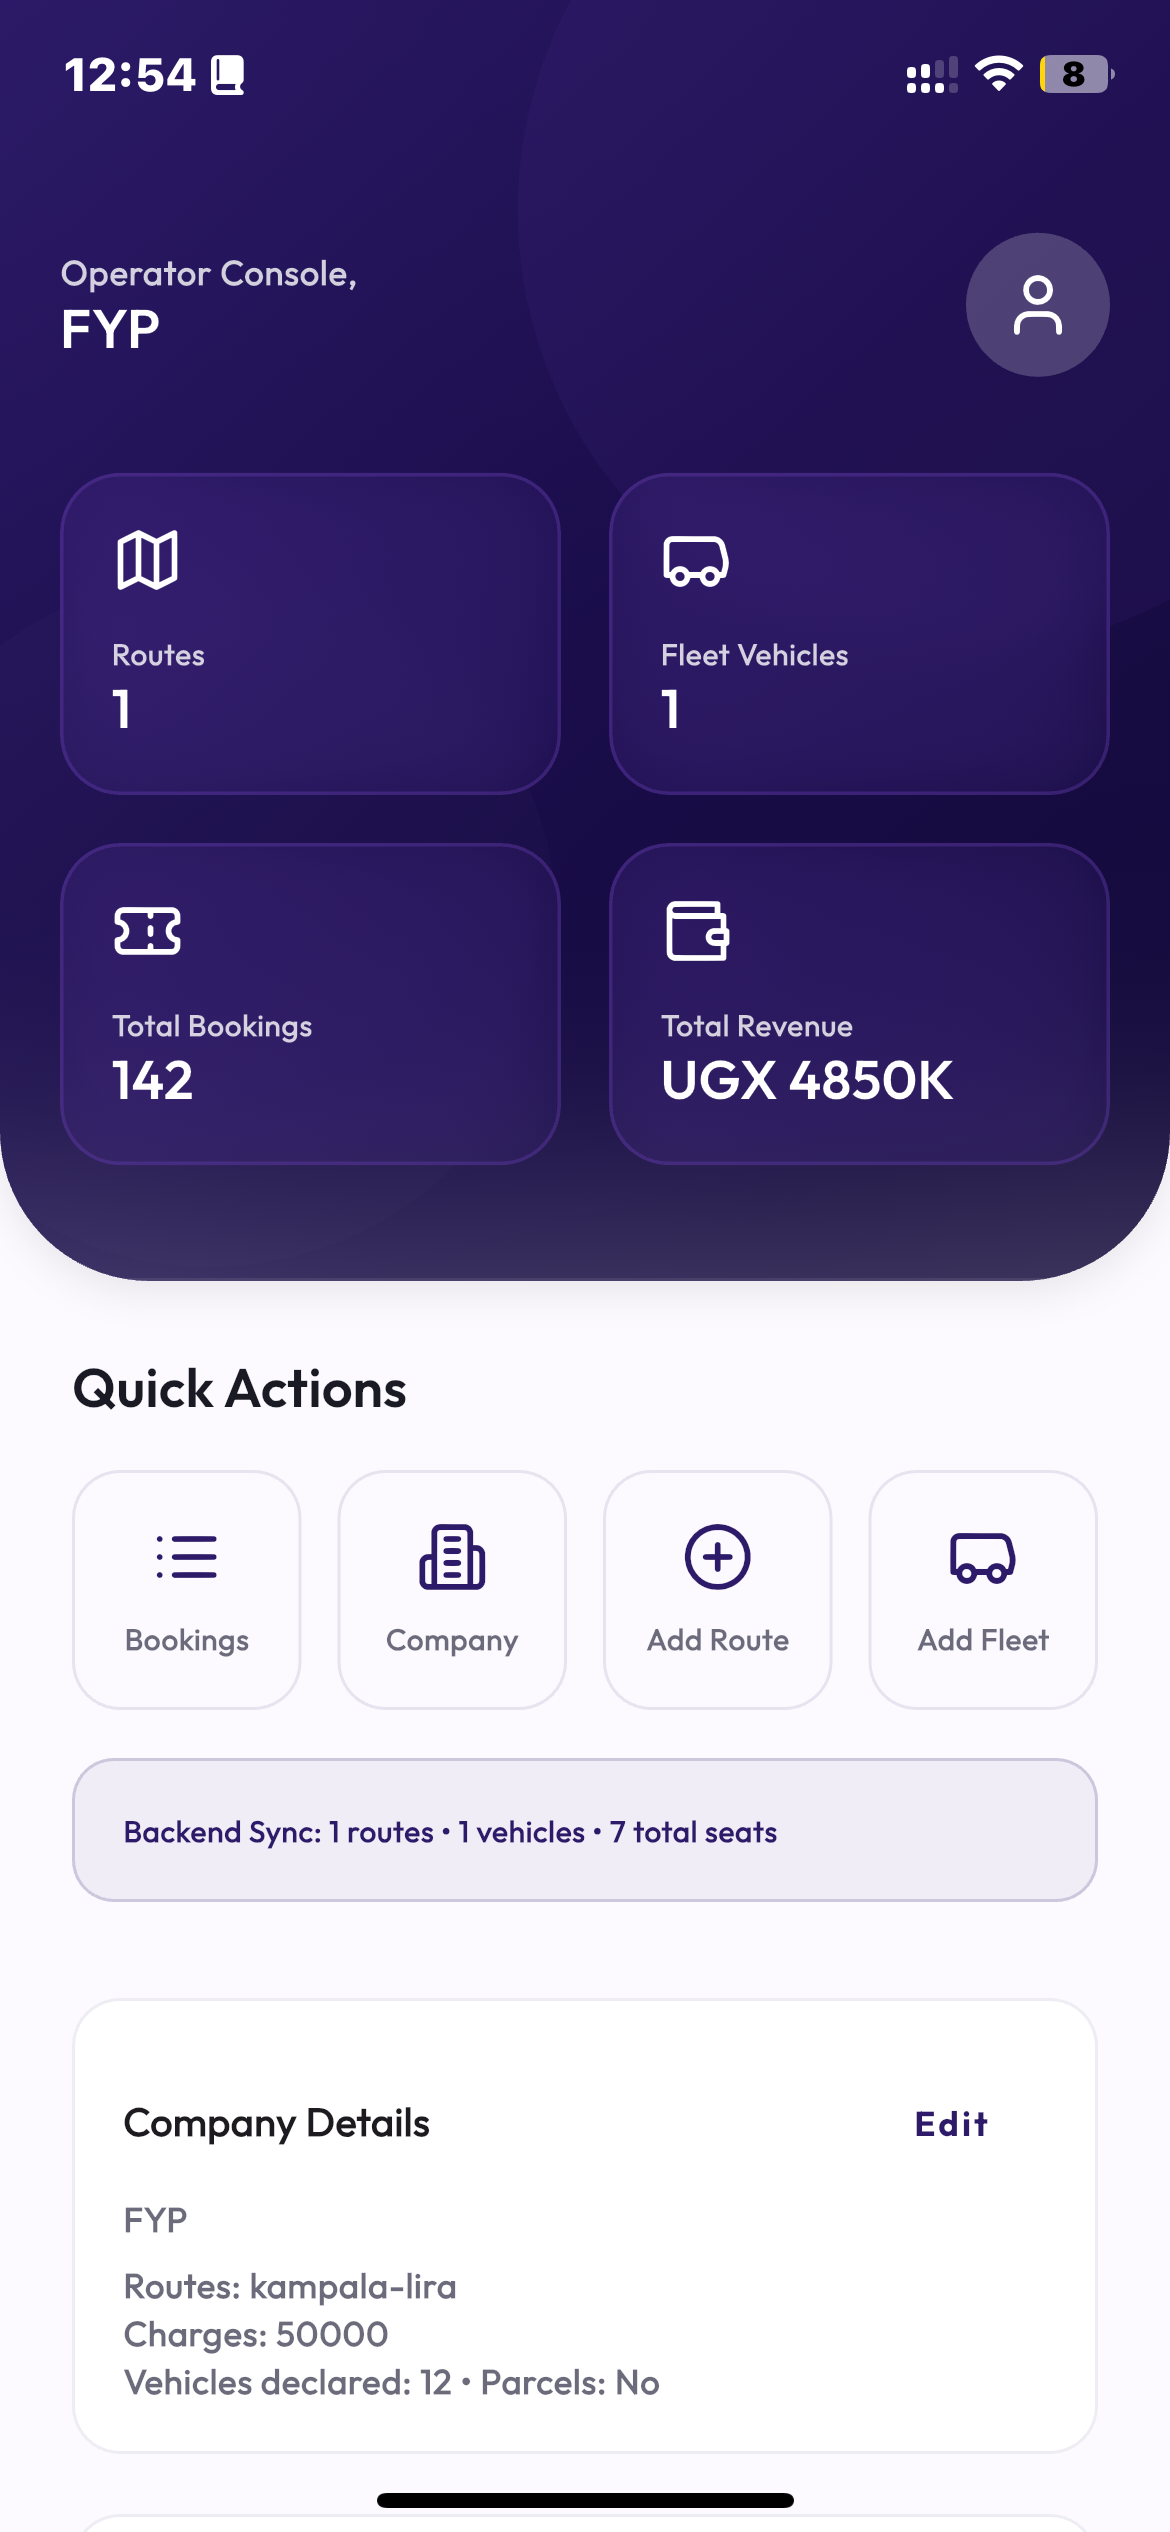
\includegraphics[width=\linewidth]{images/FYP/Operator dashboard.PNG}
    \caption{Operator dashboard}
\end{subfigure}
\hfill
\begin{subfigure}{0.32\textwidth}
    \centering
    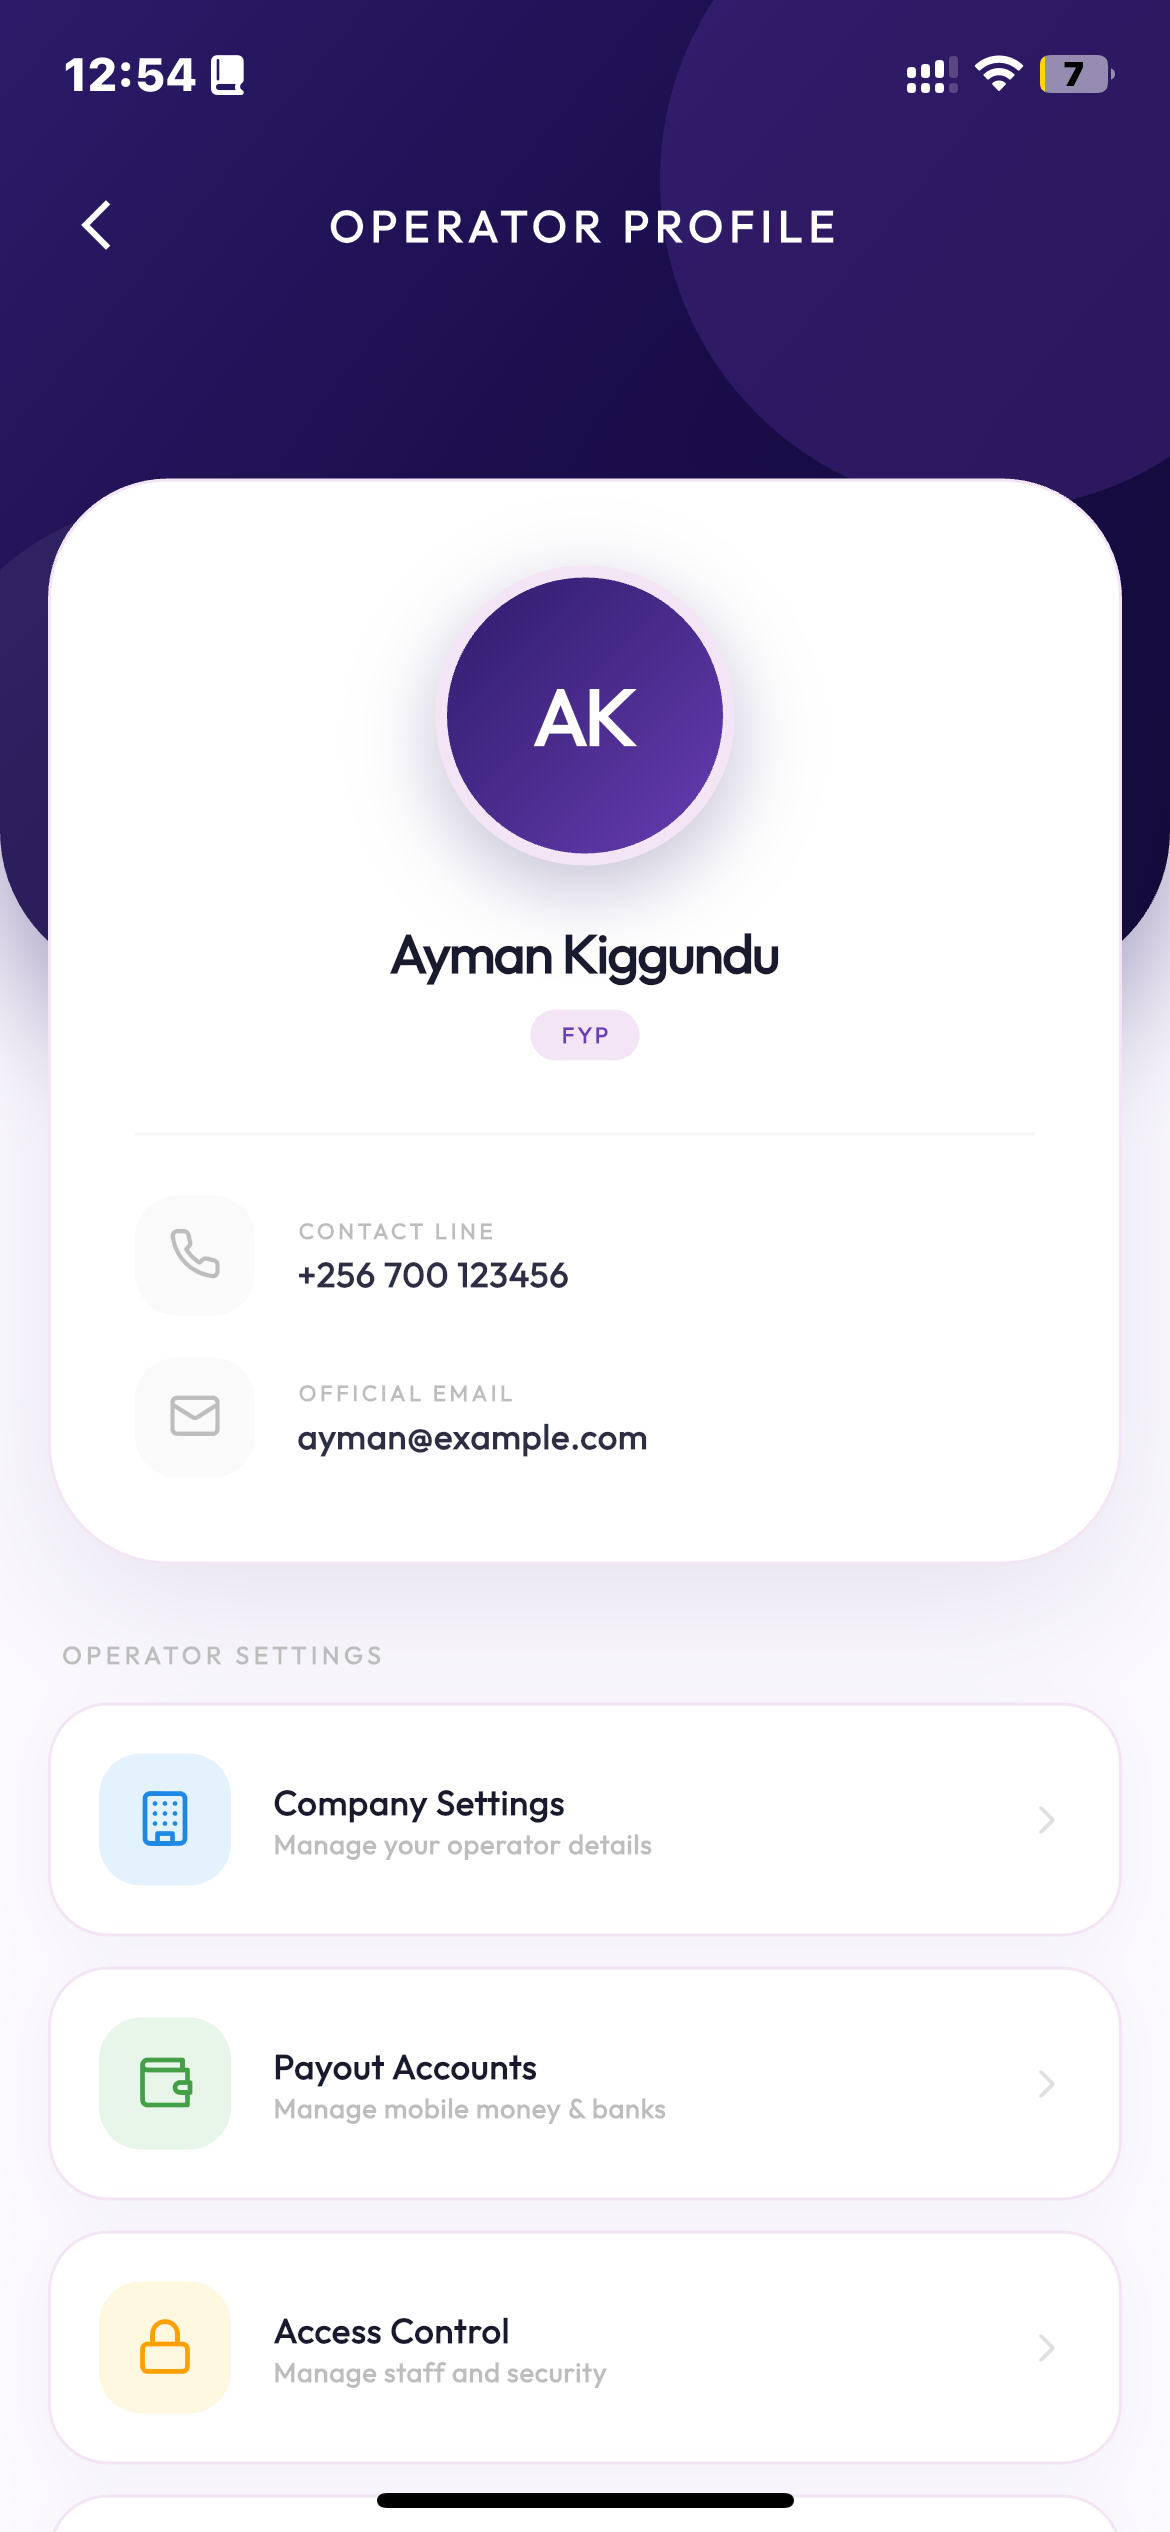
\includegraphics[width=\linewidth]{images/FYP/Operator profile.PNG}
    \caption{Operator profile}
\end{subfigure}
\hfill
\begin{subfigure}{0.32\textwidth}
    \centering
    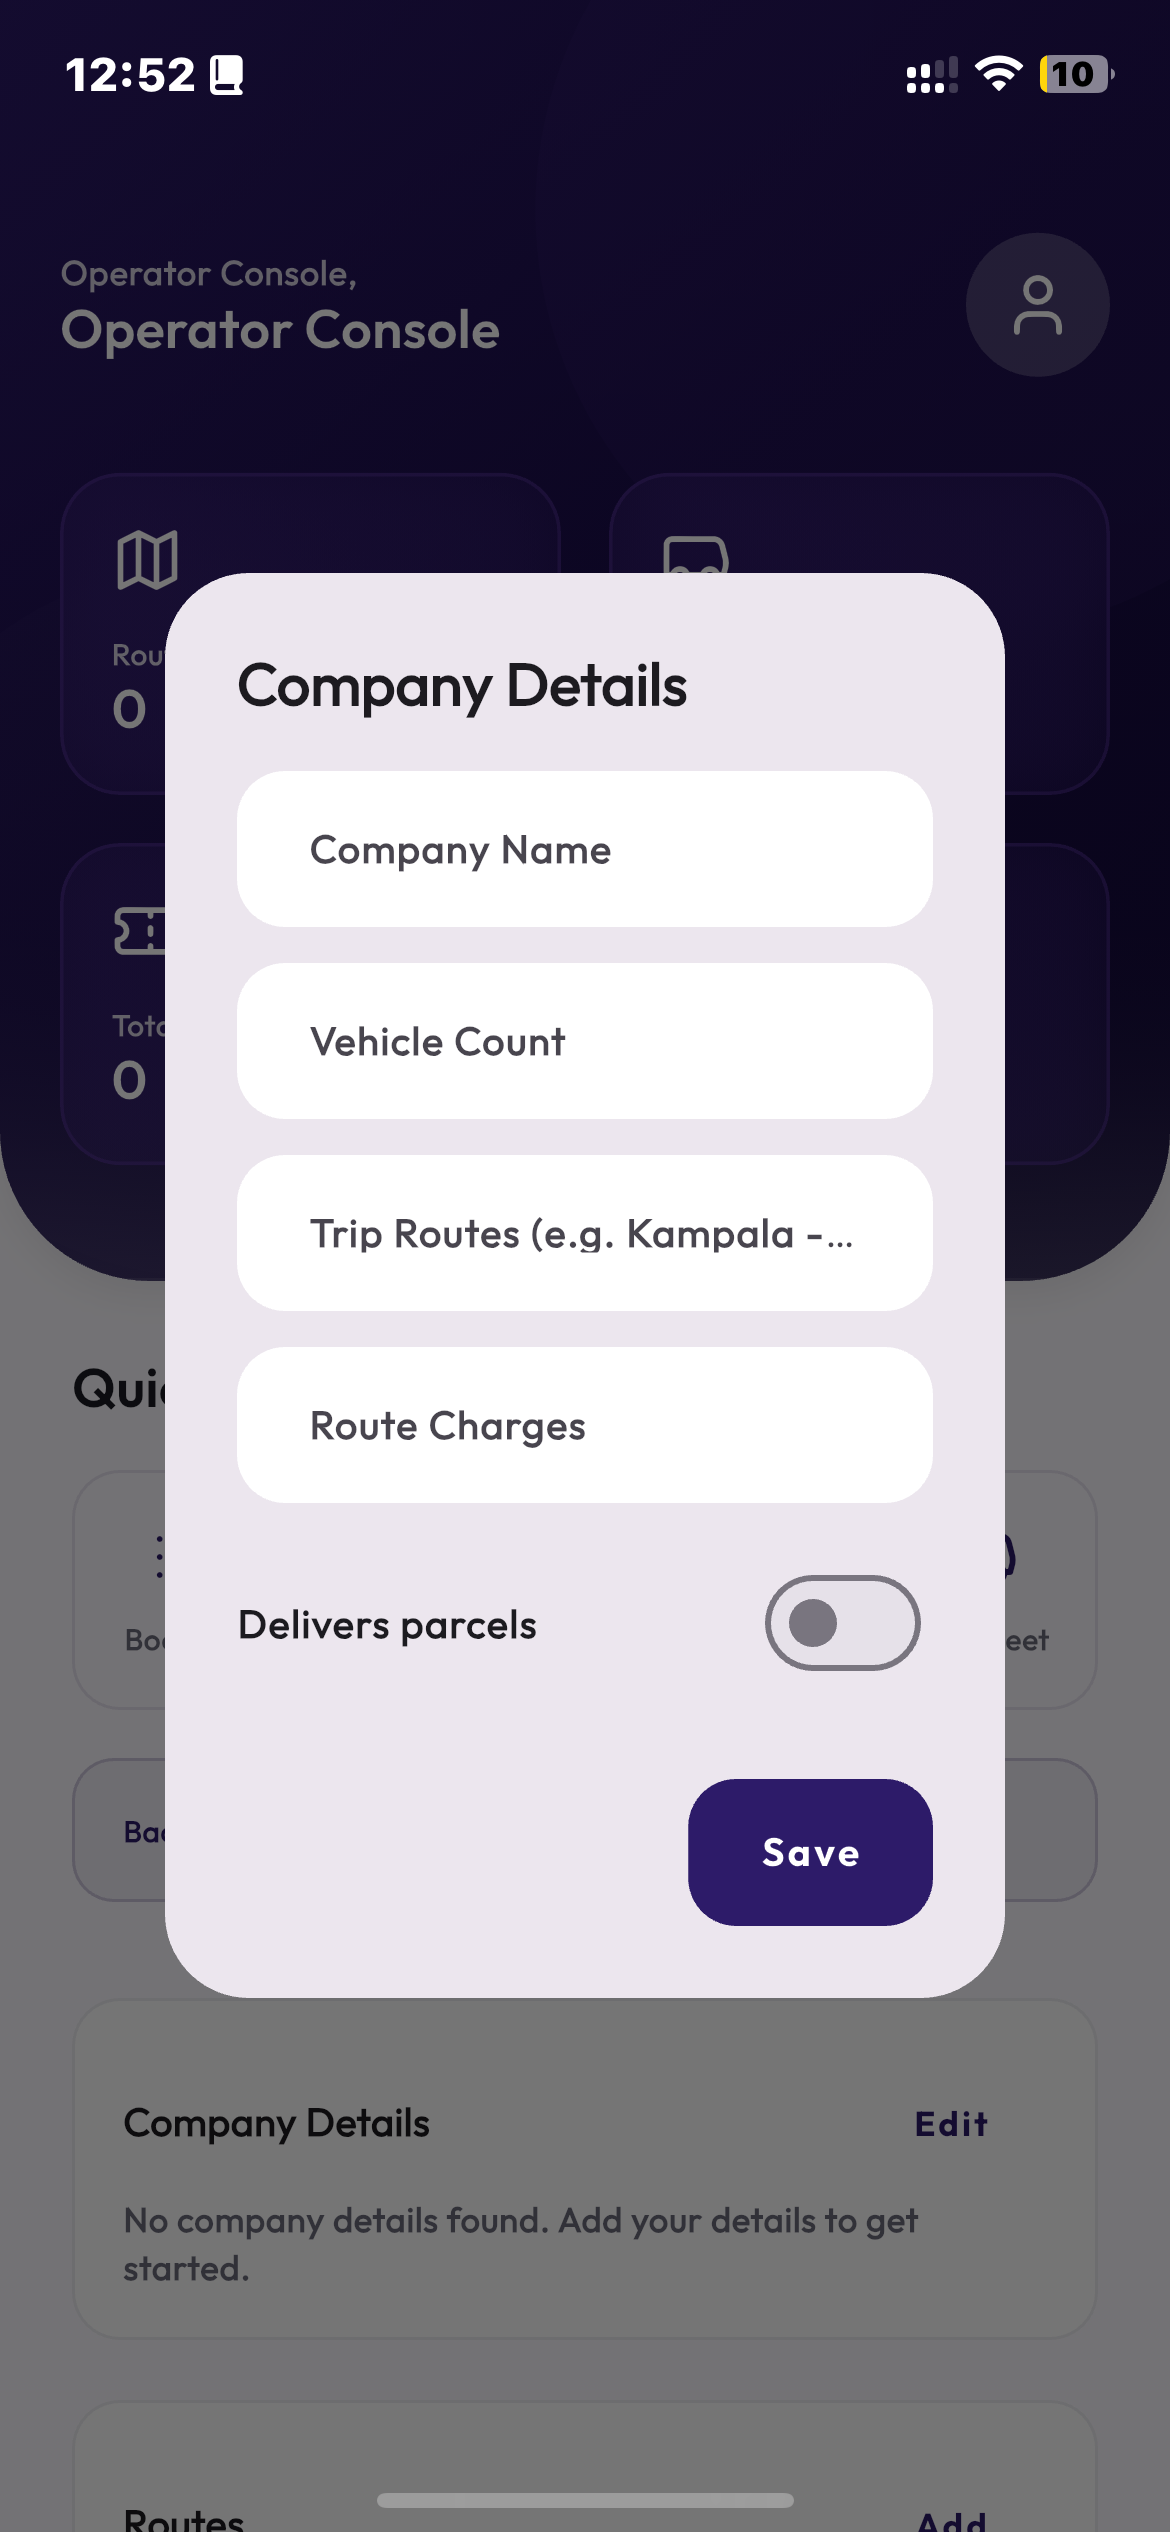
\includegraphics[width=\linewidth]{images/FYP/Company registration.PNG}
    \caption{Company registration}
\end{subfigure}

\caption{Operator interfaces}
\label{fig:operator-interfaces}

\end{figure}

\subsubsection{Passenger Actions}
Passengers can book rides by their pickup and drop-off locations, choosing a route, choose a dispatcher and confirming their booking. Passengers can also choose to book a ride for a future date and time.The app allows them to choose a seat in the taxi. The app provides a ticketing system that generates a unique ticket for each booking, which passengers can use to verify their ride and access the shuttle.During the trip, they can track the location of their shuttle in real-time and view the estimated time of arrival. They can also view their trip history, upcoming trips, and manage their profiles. The interface is designed to be simple and accessible, ensuring that users of varying technological proficiency can easily navigate and utilize the app's features. 
For parcel delivery, passengers can specify the pickup and drop-off locations, the type of parcel, the item's weight and even call for clarity on the fare to be charged. They can also track the status of their parcel in real-time and receive notifications about the delivery progress.


\begin{figure}[htbp]
\centering

\begin{subfigure}{0.32\textwidth}
    \centering
    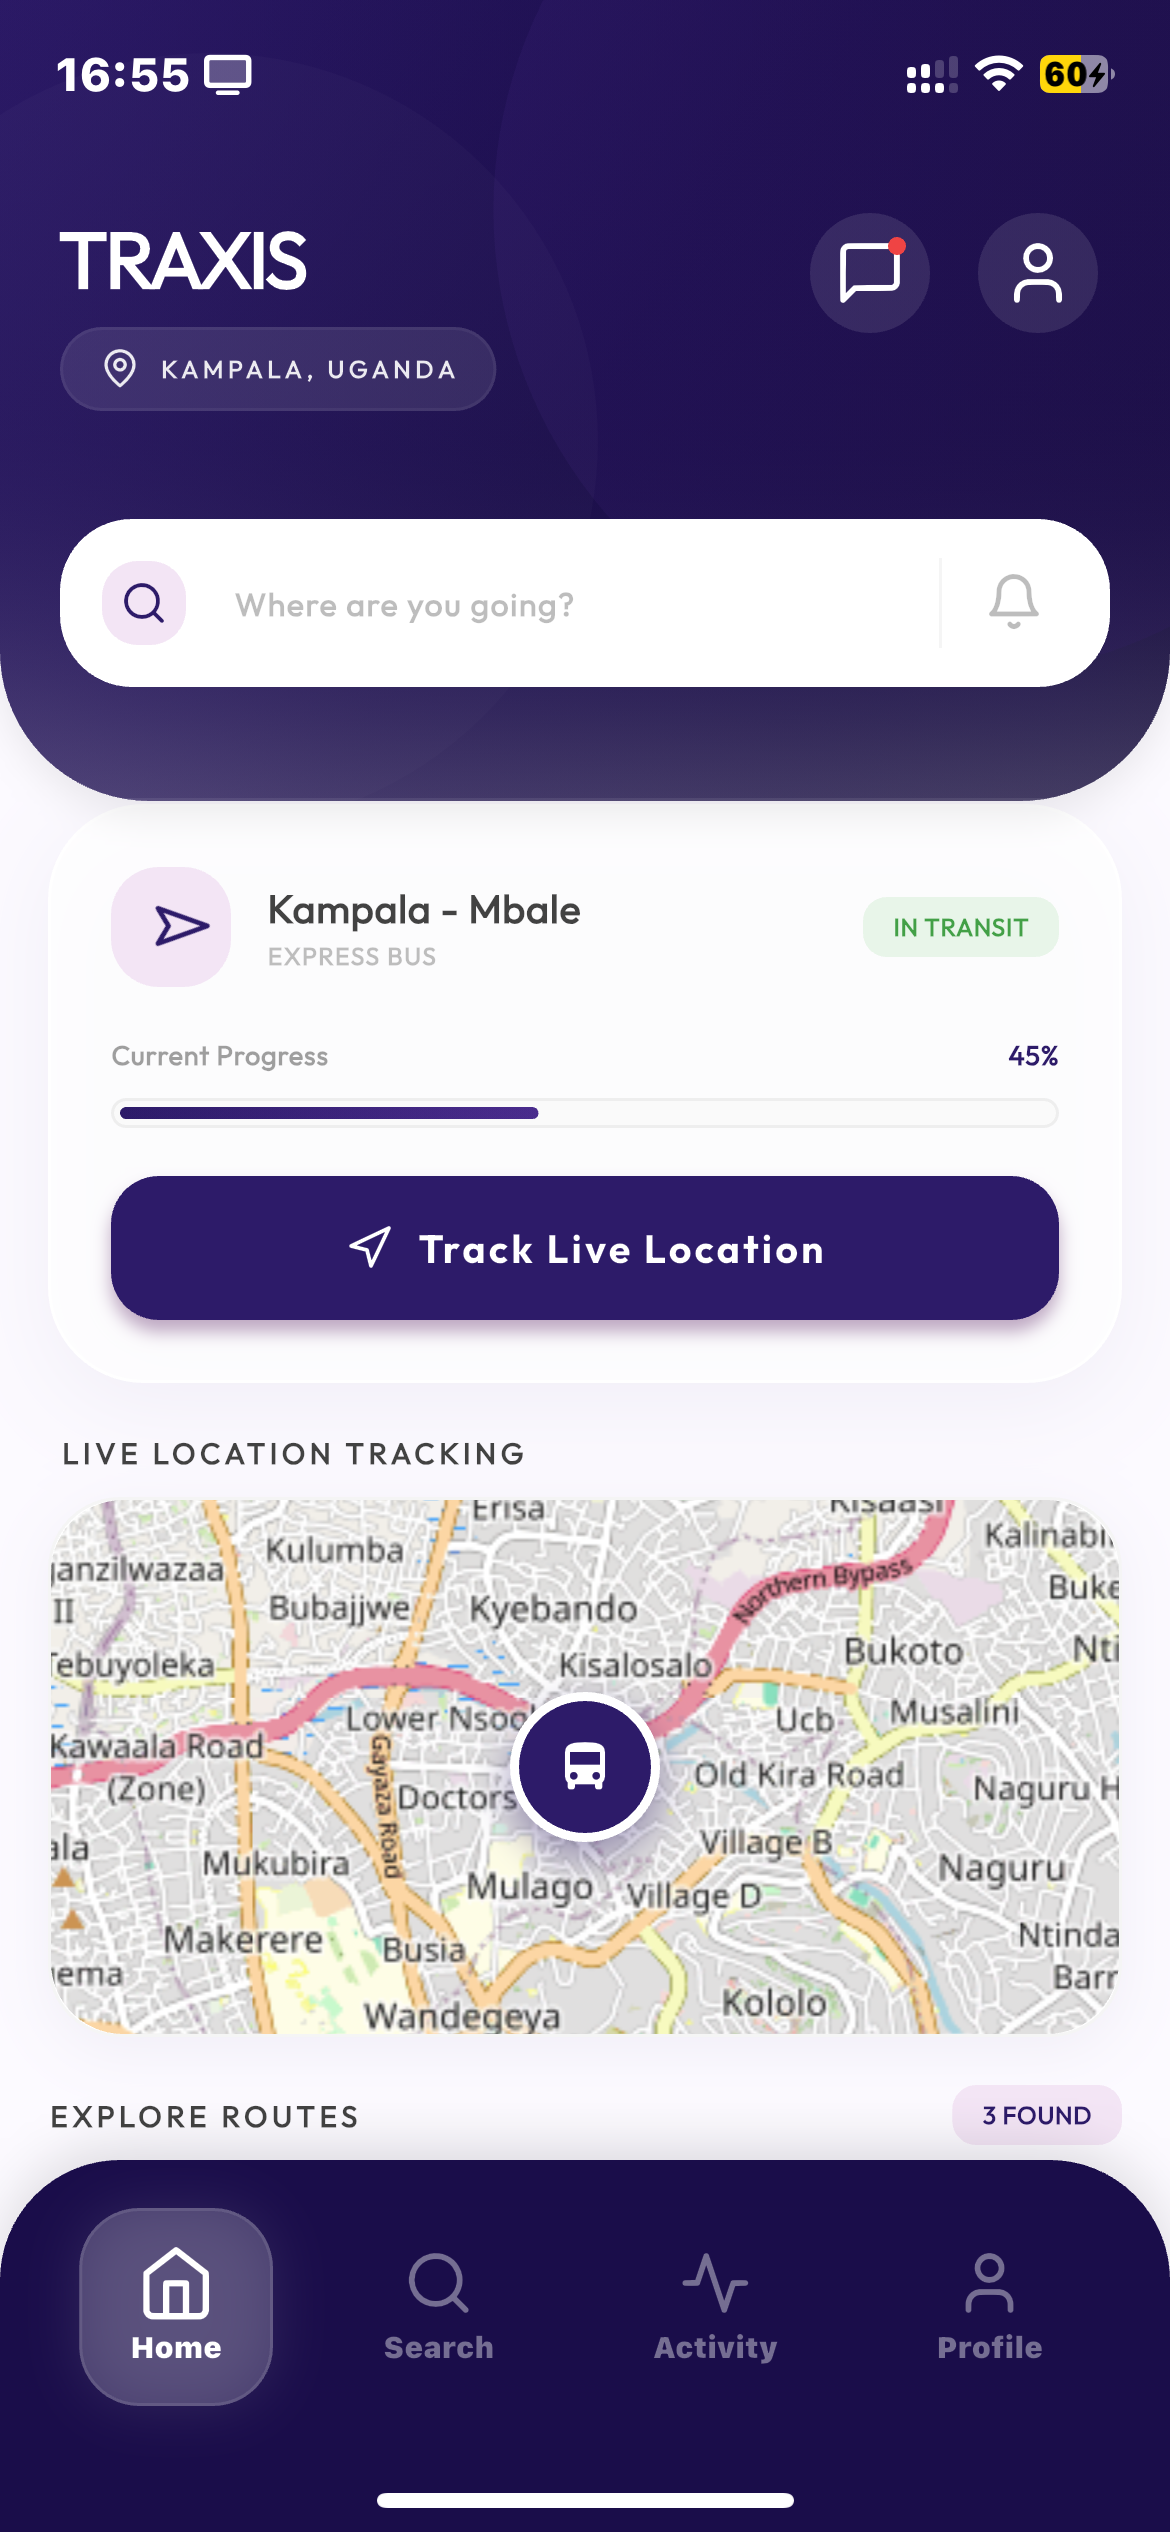
\includegraphics[width=\linewidth]{images/FYP/Passenger dashboard.PNG}
    \caption{Passenger dashboard}
\end{subfigure}
\hfill
\begin{subfigure}{0.32\textwidth}
    \centering
    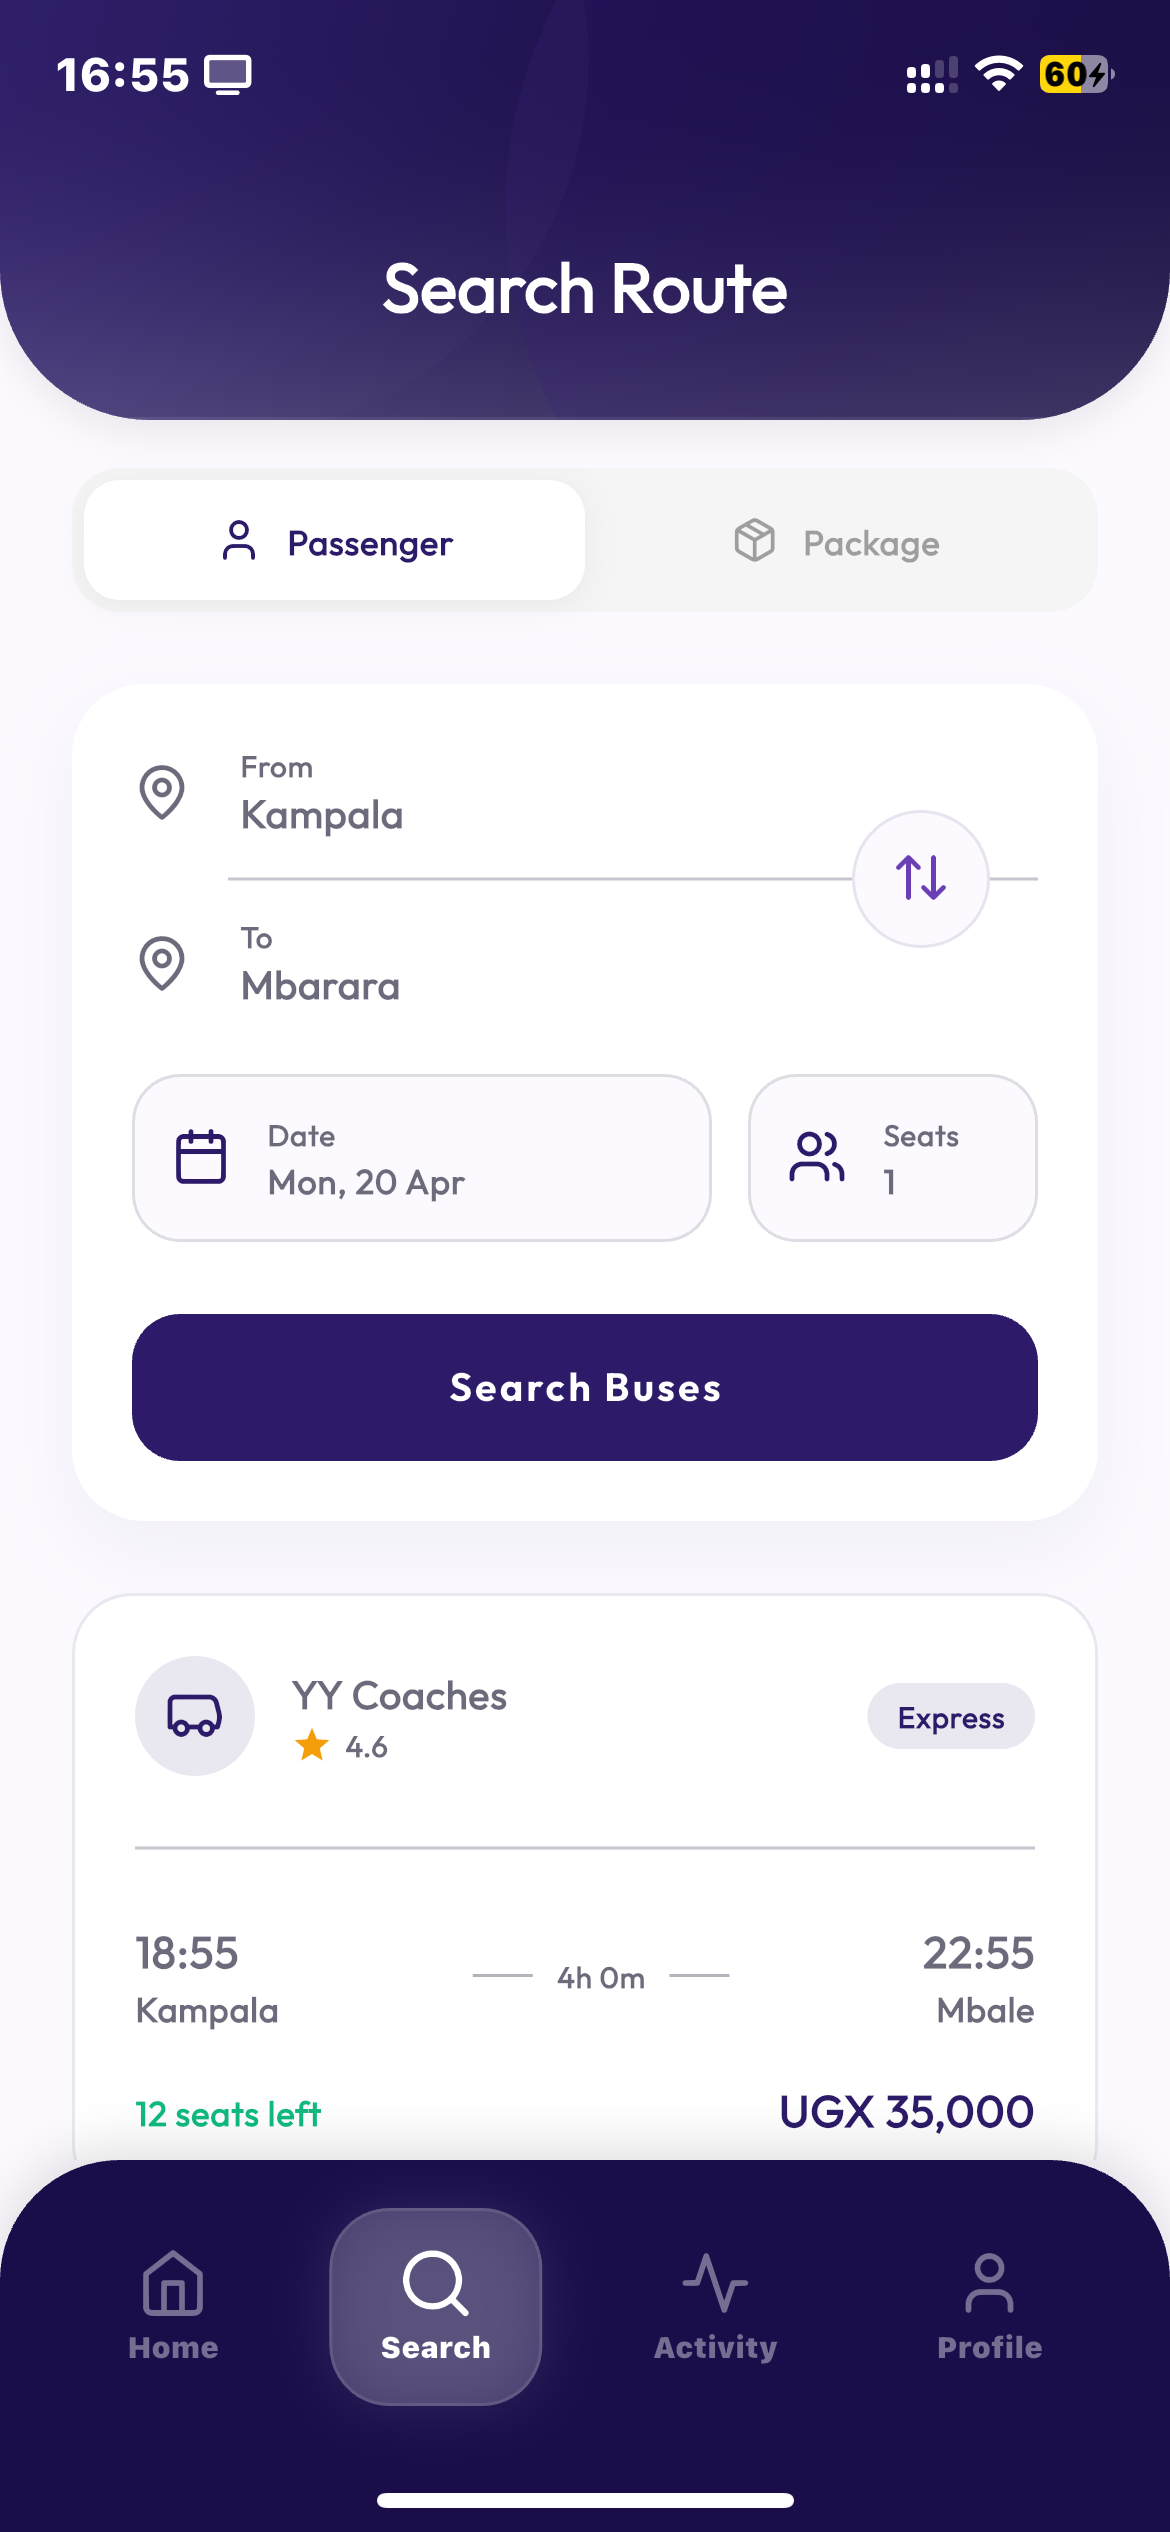
\includegraphics[width=\linewidth]{images/FYP/Route details.PNG}
    \caption{Imputting route details}
\end{subfigure}
\hfill
\begin{subfigure}{0.32\textwidth}
    \centering
    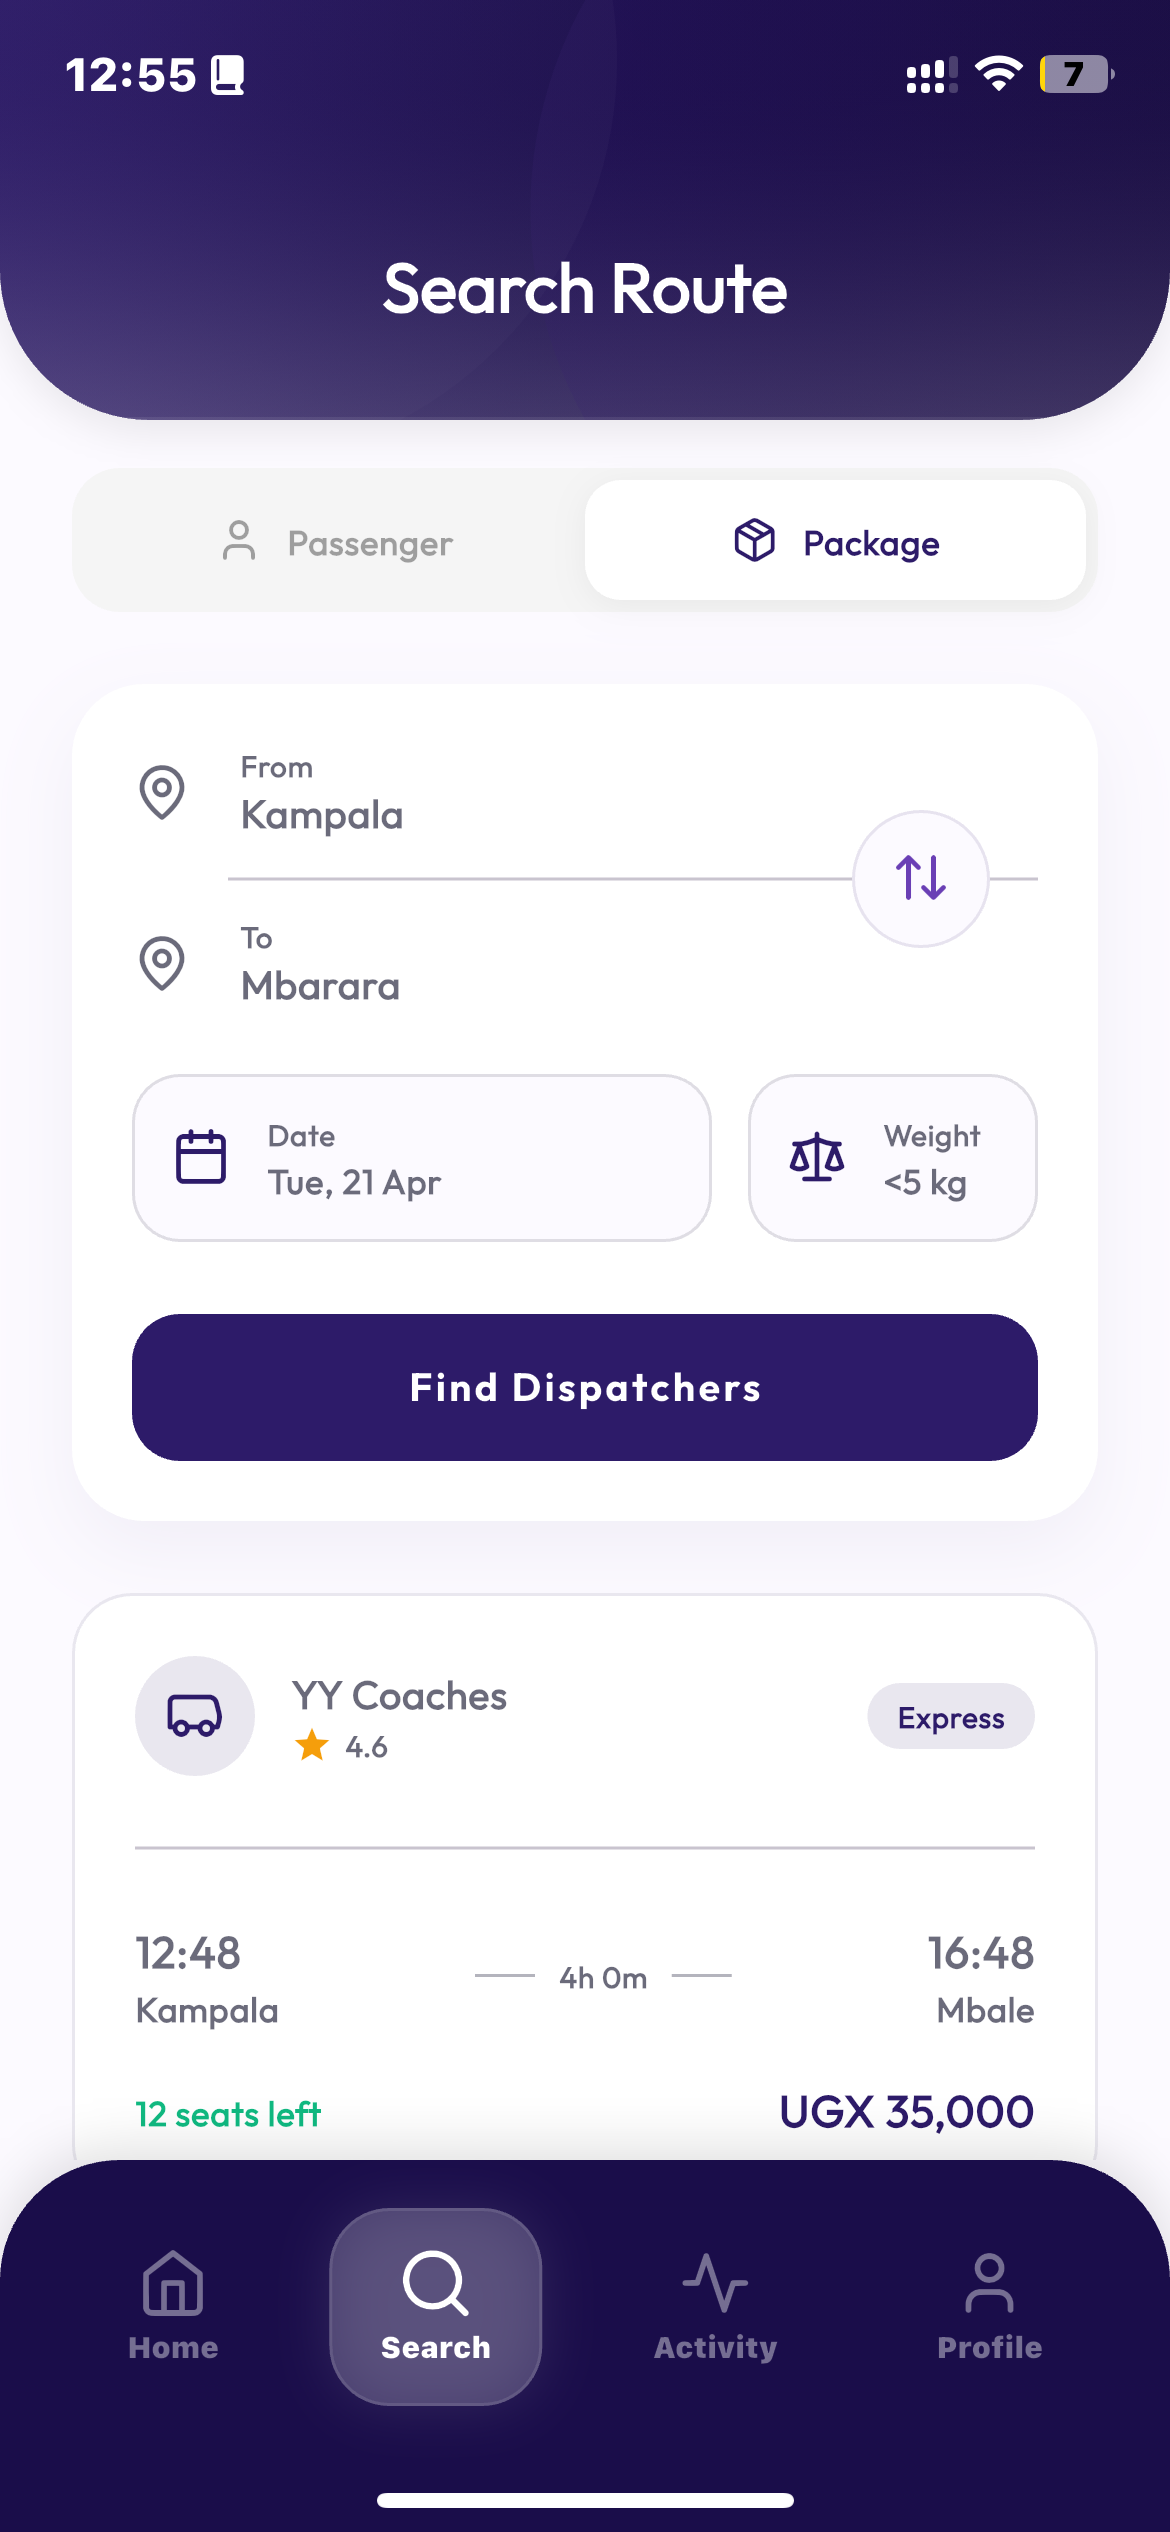
\includegraphics[width=\linewidth]{images/FYP/Parcel delivery details.PNG}
    \caption{Imputting parcel delivery details}
\end{subfigure}

\caption{Operator interfaces}
\label{fig:passenger-interfaces}

\end{figure}

\begin{figure}[htbp]
\centering

\begin{subfigure}{0.32\textwidth}
    \centering
    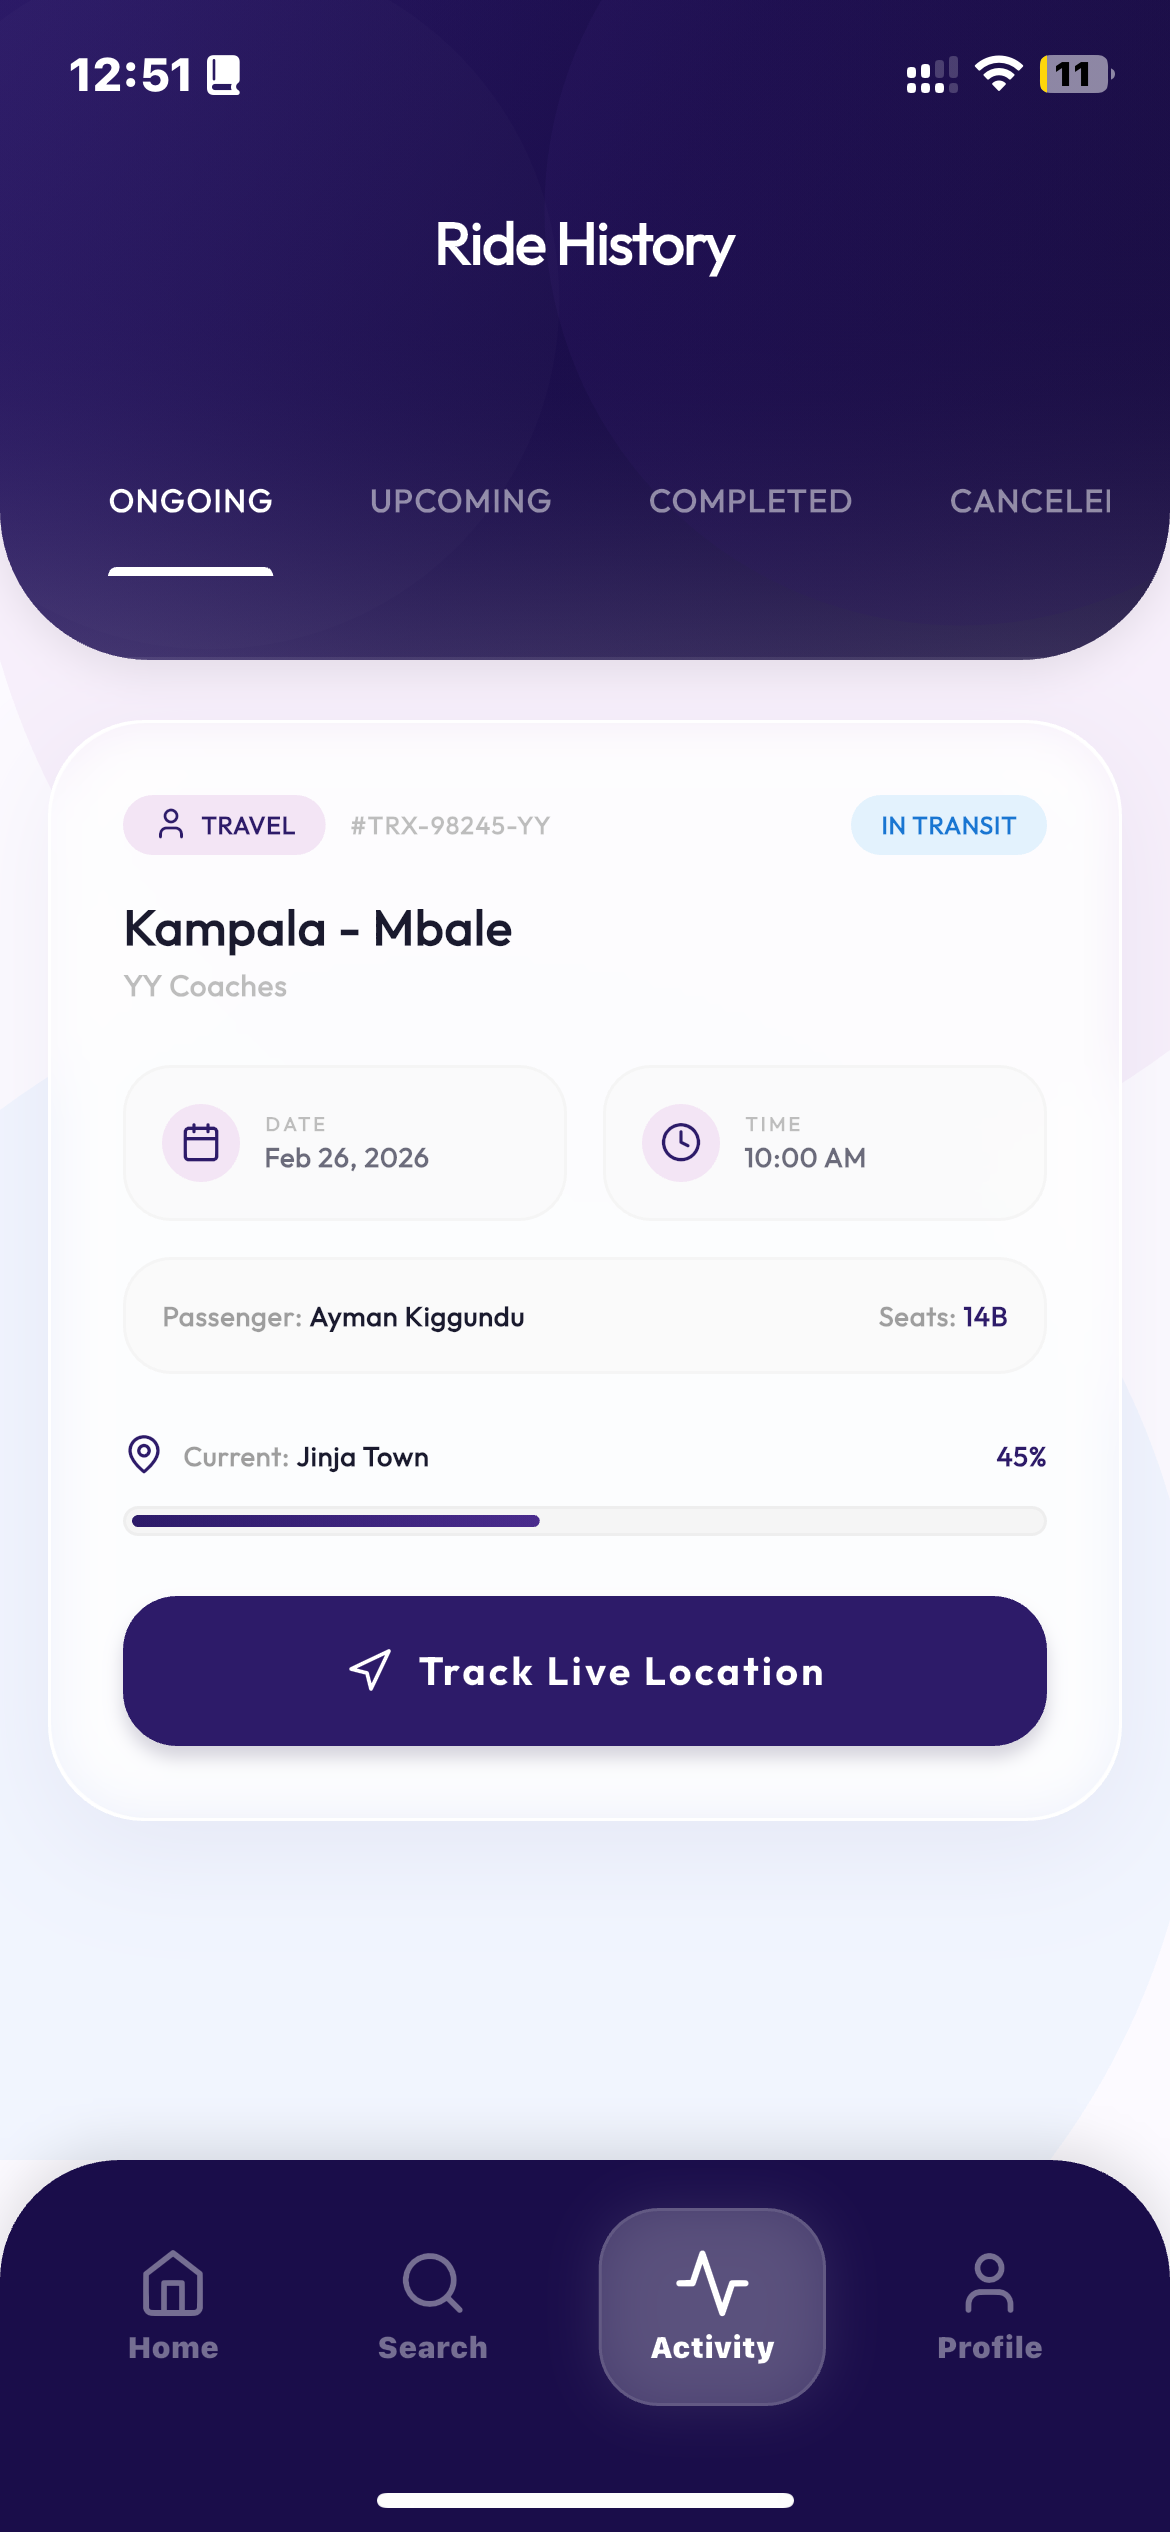
\includegraphics[width=\linewidth]{images/FYP/Ongoing trip tracking.PNG}
    \caption{Ongoing trip tracking}
\end{subfigure}
\hfill
\begin{subfigure}{0.32\textwidth}
    \centering
    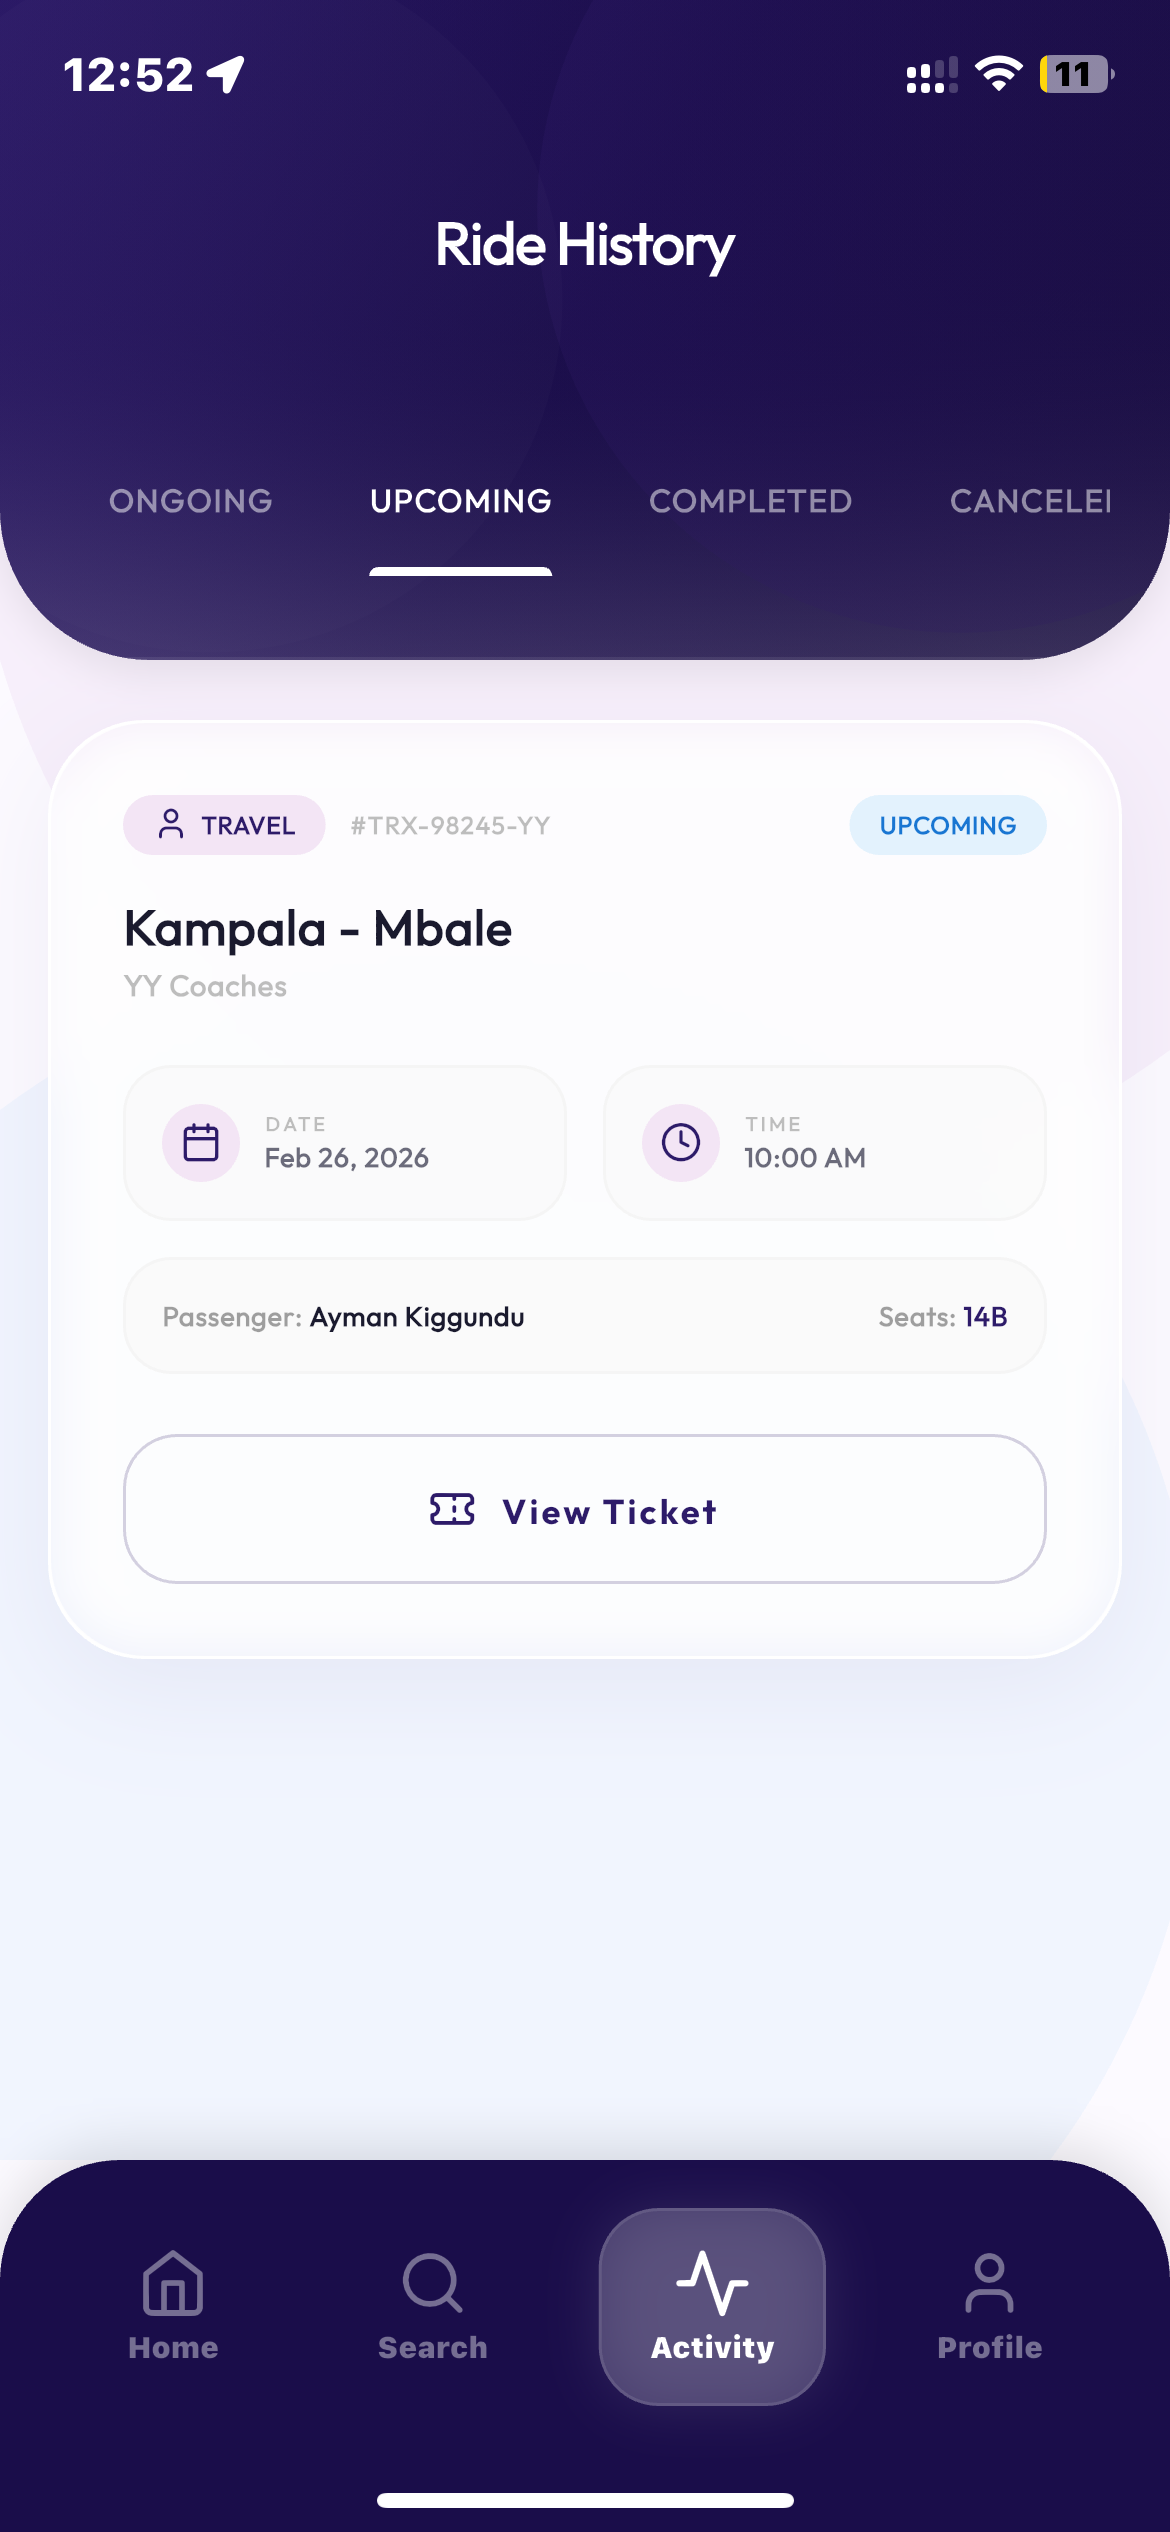
\includegraphics[width=\linewidth]{images/FYP/Tracking upcoming trips.PNG}
    \caption{Tracking upcoming trips}
\end{subfigure}
\hfill
\begin{subfigure}{0.32\textwidth}
    \centering
    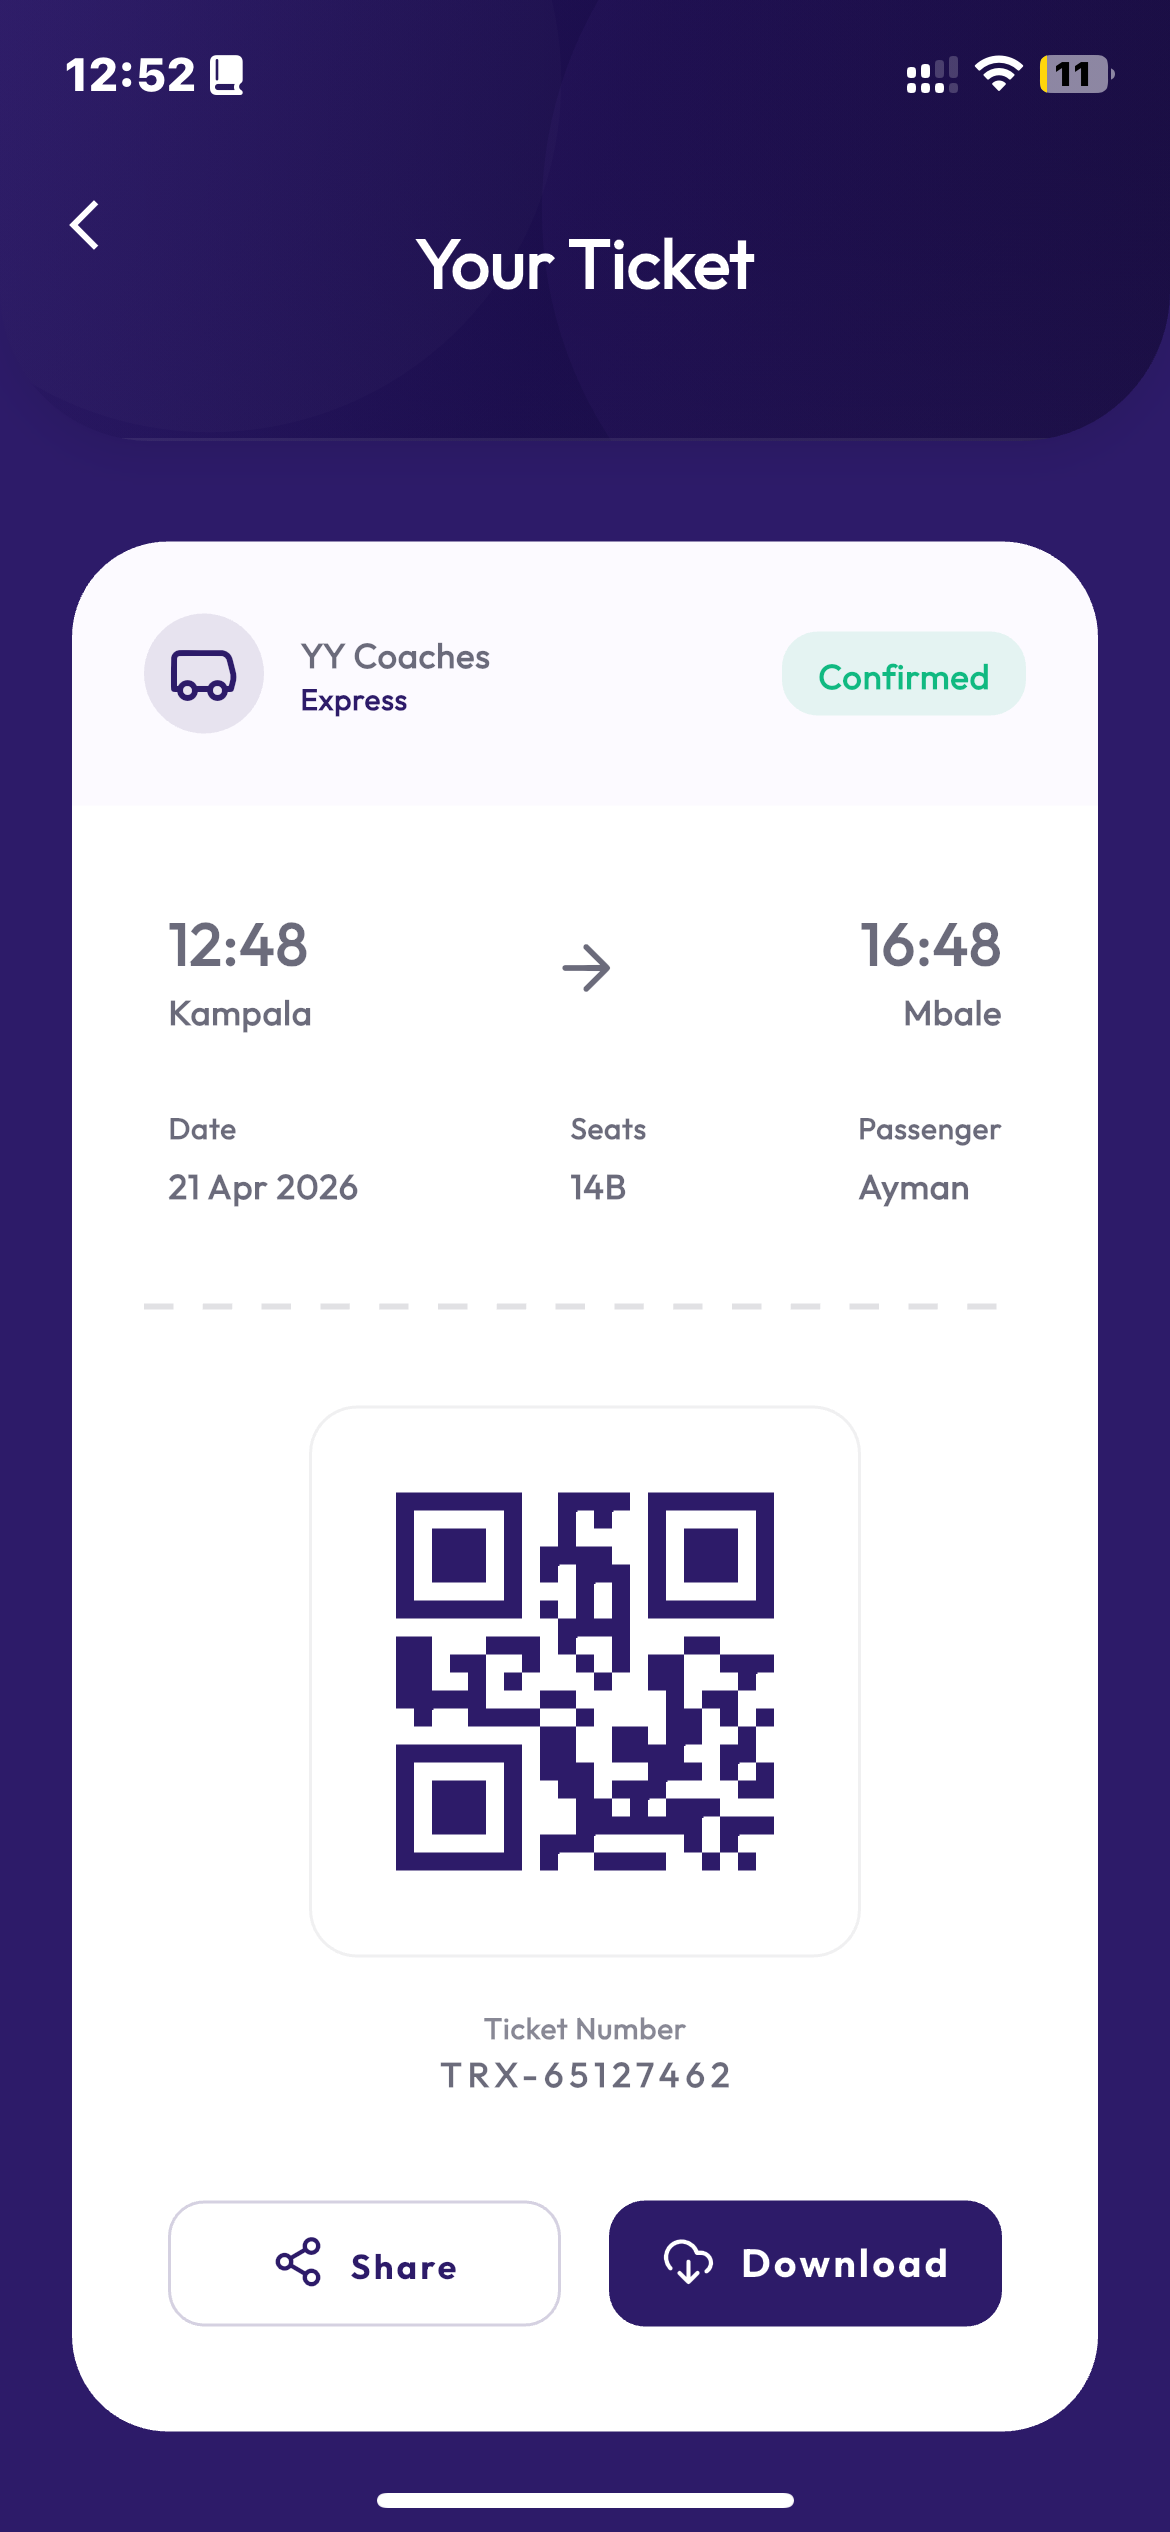
\includegraphics[width=\linewidth]{images/FYP/Digital Ticket.PNG}
    \caption{Digital ticket}
\end{subfigure}

\caption{Operator interfaces}
\label{fig:passenger-interfaces}

\end{figure}

\subsection{System Testing and Validation}
To ensure a robust and reliable system, testing was performed continuously at every stage of development. The approach emphasizes early detection of defects and validation of functionality rather than deferring testing until the end of the project. This proactive
strategy guarantees that issues are identified and resolved promptly, maintaining high system
quality and reliability. 

\subsection{Testing strategy and tools}
The system underwent multiple layers of testing, covering individual components, integration points, overall system performance, and real-world usability:

\textbf{Unit testing}: Individual components were validated using unit tests to ensure that
each module behaved as expected in isolation. For the backend, pytest was used to test Python and Django functionality, while the frontend Flutter applications employed flutter test and mockito for widget and logic testing. The development goal was to achieve greater than eighty five percent coverage on critical paths, ensuring that essential features functioned reliably under a variety of conditions.

\textbf{Integration testing}: Integration tests verified that different modules interacted correctly and that API contracts were honored. Backend APIs were tested using structured Postman collections to ensure correct request-response behavior, while end-to-end flows for
mobile applications were tested using the Flutter Integration Driver. This ensured that
data flowed seamlessly between clients, the backend, and external services.

\textbf{System and Load Testing}: To evaluate system performance under realistic usage conditions, load tests simulated up to 200 concurrent driver and passenger sessions using tools such as k6 or Locust. Performance metrics, including GPS update latency, were monitored to confirm that updates remained under 4 seconds even on 3G networks. These tests validated the system’s scalability, responsiveness, and resilience under peak loads.

\textbf{Real-World Field Testing}: 
Controlled simulations alone were not sufficient to capture the practical challenges faced in private shuttle operations, particularly those identified during the interview with HillsLink Express. Instead, the system design and evaluation were guided by real-world operational scenarios derived from the interview findings.

These scenarios included common activities such as seat booking via phone, managing no-shows, handling mid-route passenger drop-offs, coordinating parcel deliveries, and responding to frequent customer inquiries about vehicle location and delivery status. By modelling these real-life interactions within the Traxis system, the study was able to assess how effectively the proposed solution addresses existing inefficiencies.

This approach ensured that the system was grounded in actual user needs and operational constraints, including limited digital literacy, reliance on phone communication, and the need for flexible booking and tracking mechanisms. As a result, Traxis was evaluated based on its ability to improve coordination, enhance transparency, and reduce operational burden within the context of private shuttle services.

\textbf{User Acceptance Testing (UAT)}: Finally, the system underwent UAT(User Acceptance Tests) with a Hillslink passenger alongside the operator. Participants performed typical tasks using the system over a two-week period. Think-aloud sessions and standardized questionnaires such as the SUS(System Usability Scale) were employed to capture qualitative and quantitative feedback, validating that the system met user needs and expectations.
The testing strategy leveraged a variety of professional tools, including Postman for API testing, Flutter DevTools for debugging and performance profiling,
Firebase Test Lab for real-device testing, Sentry for crash reporting from the earliest stages of development, and Firebase Performance Monitoring for continuous perfor
mance evaluation. 

By employing this comprehensive, multi-layered testing and validation strategy, the
Traxis system achieved high reliability, responsiveness, and usability, ensuring readiness for real-world deployment and sustained user satisfaction


% References
\addcontentsline{toc}{chapter}{References}  
\bibliographystyle{IEEEtran}
\bibliography{references}

% Appendices
\let\cleardoublepage\clearpage % Prevent new page for appendices
\begin{appendix}
    \chapter*{Appendices}
\addcontentsline{toc}{chapter}{Appendices} % Add to table of contents

\section*{Appendix A : Budget}
% \label{app:time_schedule}
The research and development of the Traxis mobile application will be conducted over a period of 3 months.

\begin{table}[h]
\centering
% \label{tab:budget}
\begin{tabularx}{\textwidth}{@{}lXr@{}}  % l = left, X = stretchable, r = right
\toprule
\textbf{Item} & \textbf{Description} & \textbf{Estimated Cost (UGX)} \\
\midrule
Internet and Communication & Research coordination, data collection, and documentation & 300,000 \\
Transport and Fieldwork & Visiting taxi parks for data collection and user feedback & 200,000 \\
Software Tools & Firebase, Google Maps API, and development plugins & 500,000 \\
Cloud Hosting & Server and database hosting for testing phase & 300,000 \\
Personnel & Allowances for research assistants and testers & 1,000,000 \\
Miscellaneous & Contingency and administrative expenses & 800,000 \\
\bottomrule
\textbf{Total} & & \textbf{3,100,000} \\
\end{tabularx}
\caption{Estimated Project Budget}
\end{table}


\clearpage
% \section*{Appendix B: Budget}
% \label{app:budget}

% The estimated budget for the proposed Traxis system is outlined below. The costs are indicative and will guide resource allocation during implementation.

% \begin{table}[h]
% \centering
% \caption{Proposed Research Work Plan}
% \label{tab:work_plan}
% \begin{tabularx}{\textwidth}{@{}lXl@{}}
% \toprule
% \textbf{Phase} & \textbf{Description} & \textbf{Timeline} \\
% \midrule
% \textbf{Semester I: Research and Documentation} & & \\
% Literature Review & Review related work and identify research gaps & Month 1 \\
% Requirements Gathering & Conduct interviews and surveys with drivers and passengers & Month 2 \\
% System Design & Develop system architecture, data flow diagrams, and UI prototypes & Month 3 \\
% \midrule
% \textbf{Semester II: Development and Testing} & & \\
% Development & Implement backend and mobile applications using Agile sprints & Months 4–5 \\
% Testing \& Evaluation & Conduct user acceptance and performance testing & Month 6 \\
% Final Report & Document results and prepare presentation & End of Month 6 \\
% \bottomrule
% \end{tabularx}
% \end{table}


% \clearpage
% \section*{Appendix B: Research Work Plan}
% \label{app:work_plan}

% The proposed research and development work plan is outlined below, aligning activities with the academic semesters.

% \begin{table}[h]
% \centering
% \caption{Proposed Research Work Plan}
% \label{tab:work_plan}
% \begin{tabularx}{\textwidth}{@{}lXl@{}} % <-- X handles wrapping
% \toprule
% \textbf{Phase} & \textbf{Description} & \textbf{Timeline} \\
% \midrule
% \textbf{Semester I: Research and Documentation} & & \\
% Literature Review & Review related work and identify research gaps & Month 1 \\
% Requirements Gathering & Conduct interviews and surveys with drivers and passengers & Month 2 \\
% System Design & Develop system architecture, data flow diagrams, and UI prototypes & Month 3 \\
% \midrule
% \textbf{Semester II: Development and Testing} & & \\
% Development & Implement backend and mobile applications using Agile sprints & Months 4--5 \\
% Testing \& Evaluation & Conduct user acceptance and performance testing & Month 6 \\
% Final Report & Document results and prepare presentation & End of Month 6 \\
% \bottomrule
% \end{tabularx}
% \end{table}

    \section*{Appendix B: Event Scheduling (Workplan)}

This appendix presents the project workplan outlining the planned activities for the development of the Traxis system. The workplan is organized chronologically and aligns with the Agile-inspired methodology described in Chapter 4. It defines the scheduled development events, their durations, and intended outputs, providing a structured roadmap for the successful execution of the project.

\subsection*{Month 1: Foundation Phase (January 2026)}

\textbf{Activity 1: Backend and Database Setup} \\
\textit{Scheduled Period: 1 January 2026 – 14 January 2026} \\
During this period, the project team will establish the foundational backend infrastructure for the system. This will include configuring the Django backend framework, setting up the PostgreSQL database with PostGIS extensions, defining core data models, and creating initial RESTful API endpoints. The expected outcome will be a functional backend environment capable of supporting authentication, data persistence, and future feature development.

\textbf{Activity 2: Authentication and Location Services Implementation} \\
\textit{Scheduled Period: 15 January 2026 – 31 January 2026} \\
This activity will focus on implementing secure authentication mechanisms and geolocation services. Firebase Authentication will be integrated to support phone-number-based user login, while Google Maps APIs will be configured for real-time location tracking and routing. Backend logic for managing user sessions and location updates will be implemented to support subsequent ride-matching functionality.

\subsection*{Month 2: Core Interaction Phase (February 2026)}

\textbf{Activity 3: User Interface and Authentication Workflow Development} \\
\textit{Scheduled Period: 1 February 2026 – 14 February 2026} \\
During this phase, the client-side applications will be developed using Flutter. User interface components, navigation flows, and authentication workflows for both passengers and drivers will be implemented from a shared codebase. The primary objective will be to deliver a functional, responsive, and user-friendly mobile interface capable of interacting securely with backend services.

\textbf{Activity 4: Ride Management Logic and AI Integration} \\
\textit{Scheduled Period: 15 February 2026 – 28 February 2026} \\
This activity will involve implementing the core ride management features of the system. Ride request handling, driver availability broadcasting, and passenger–driver matching logic will be developed within the backend. AI services will be integrated through MCP to support predictive matching and demand-aware allocation. Real-time notifications will be enabled using Firebase Cloud Messaging to ensure timely communication between system components.

\subsection*{Month 3: System Enhancement and Finalization Phase (March 2026)}

\textbf{Activity 5: Analytics and Administrative Tools Development} \\
\textit{Scheduled Period: 1 March 2026 – 14 March 2026} \\
This phase will focus on the development of administrative and analytical capabilities. The Admin Portal will be implemented using Vue.js to provide tools for user management, trip monitoring, and system analytics. Supporting backend endpoints for reporting, logging, and administrative operations will be completed to enable effective system oversight.

\textbf{Activity 6: Performance Optimization, Accessibility, and System Validation} \\
\textit{Scheduled Period: 15 March 2026 – 31 March 2026} \\
The final activity will concentrate on system refinement and deployment readiness. Performance optimization will be conducted across the backend and mobile applications, including database tuning and background task optimization. Accessibility enhancements will be implemented to improve usability for diverse user groups. Comprehensive testing, bug fixing, and final system validation will be carried out to ensure compliance with project requirements.

\subsection*{Workplan Summary}

The proposed workplan will ensure a phased and systematic approach to system development, progressing from foundational setup to core functionality and final optimization. By adhering to clearly defined activities and timelines, the project will maintain effective coordination, reduce development risks, and support the timely delivery of the Traxis system in accordance with the proposed methodology.
\end{appendix}

\end{document}